% ******************************* PhD Thesis Template **************************
% Please have a look at the README.md file for info on how to use the template

\documentclass[a4paper,12pt,times,numbered,print,index]{Classes/PhDThesisPSnPDF}

% ******************************************************************************
% ******************************* Class Options ********************************
% *********************** See README for more details **************************
% ******************************************************************************

% `a4paper'(The University of Cambridge PhD thesis guidelines recommends a page
% size a4 - default option) or `a5paper': A5 Paper size is also allowed as per
% the Cambridge University Engineering Deparment guidelines for PhD thesis
%
% `11pt' or `12pt'(default): Font Size 10pt is NOT recommended by the University
% guidelines
%
% `oneside' or `twoside'(default): Printing double side (twoside) or single
% side.
%
% `print': Use `print' for print version with appropriate margins and page
% layout. Leaving the options field blank will activate Online version.
%
% `index': For index at the end of the thesis
%
% `draftclassic': For draft mode without loading any images (same as draft in book)
%
% `draft': Special draft mode with line numbers, images, and water mark with
% timestamp and custom text. Position of the text can also be modified.
%
% `abstract': To generate only the title page and abstract page with
% dissertation title and name, to submit to the Student Registry
%
% `chapter`: This option enables only the specified chapter and it's references
%  Useful for review and corrections.
%
% ************************* Custom Page Margins ********************************
%
% `custommargin`: Use `custommargin' in options to activate custom page margins,
% which can be defined in the preamble.tex. Custom margin will override
% print/online margin setup.
%
% *********************** Choosing the Fonts in Class Options ******************
%
% `times' : Times font with math support. (The Cambridge University guidelines
% recommend using times)
%
% `fourier': Utopia Font with Fourier Math font (Font has to be installed)
%            It's a free font.
%
% `customfont': Use `customfont' option in the document class and load the
% package in the preamble.tex
%
% default or leave empty: `Latin Modern' font will be loaded.
%
% ********************** Choosing the Bibliography style ***********************
%
% `authoryear': For author-year citation eg., Krishna (2013)
%
% `numbered': (Default Option) For numbered and sorted citation e.g., [1,5,2]
%
% `custombib': Define your own bibliography style in the `preamble.tex' file.
%              `\RequirePackage[square, sort, numbers, authoryear]{natbib}'.
%              This can be also used to load biblatex instead of natbib
%              (See Preamble)
%
% **************************** Choosing the Page Style *************************
%
% `default (leave empty)': For Page Numbers in Header (Left Even, Right Odd) and
% Chapter Name in Header (Right Even) and Section Name (Left Odd). Blank Footer.
%
% `PageStyleI': Chapter Name next & Page Number on Even Side (Left Even).
% Section Name & Page Number in Header on Odd Side (Right Odd). Footer is empty.
%
% `PageStyleII': Chapter Name on Even Side (Left Even) in Header. Section Number
% and Section Name in Header on Odd Side (Right Odd). Page numbering in footer

% Uncomment to change page style
\pagestyle{PageStyleII}

% ********************************** Preamble **********************************
% Preamble: Contains packages and user-defined commands and settings
% ******************************************************************************
% ****************************** Custom Margin *********************************

% Add `custommargin' in the document class options to use this section
% Set {innerside margin / outerside margin / topmargin / bottom margin}  and
% other page dimensions
\ifsetCustomMargin
  \RequirePackage[left=37mm,right=30mm,top=35mm,bottom=30mm]{geometry}
  \setFancyHdr % To apply fancy header after geometry package is loaded
\fi

% Add spaces between paragraphs
%\setlength{\parskip}{0.5em}
% Ragged bottom avoids extra whitespaces between paragraphs
\raggedbottom
% To remove the excess top spacing for enumeration, list and description
%\usepackage{enumitem}
%\setlist[enumerate,itemize,description]{topsep=0em}

% *****************************************************************************
% ******************* Fonts (like different typewriter fonts etc.)*************

% Add `customfont' in the document class option to use this section

\ifsetCustomFont
  % Set your custom font here and use `customfont' in options. Leave empty to
  % load computer modern font (default LaTeX font).
  %\RequirePackage{helvet}

  % For use with XeLaTeX
  %  \setmainfont[
  %    Path              = ./libertine/opentype/,
  %    Extension         = .otf,
  %    UprightFont = LinLibertine_R,
  %    BoldFont = LinLibertine_RZ, % Linux Libertine O Regular Semibold
  %    ItalicFont = LinLibertine_RI,
  %    BoldItalicFont = LinLibertine_RZI, % Linux Libertine O Regular Semibold Italic
  %  ]
  %  {libertine}
  %  % load font from system font
  %  \newfontfamily\libertinesystemfont{Linux Libertine O}
\fi

% *****************************************************************************
% **************************** Custom Packages ********************************

% ************************* Algorithms and Pseudocode **************************

%\usepackage{algpseudocode}


% ********************Captions and Hyperreferencing / URL **********************

% Captions: This makes captions of figures use a boldfaced small font.
%\RequirePackage[small,bf]{caption}

\RequirePackage[labelsep=space,tableposition=top]{caption}
\renewcommand{\figurename}{Fig.} %to support older versions of captions.sty


% *************************** Graphics and figures *****************************

%\usepackage{rotating}
%\usepackage{wrapfig}

% Uncomment the following two lines to force Latex to place the figure.
% Use [H] when including graphics. Note 'H' instead of 'h'
%\usepackage{float}
%\restylefloat{figure}

% Subcaption package is also available in the sty folder you can use that by
% uncommenting the following line
% This is for people stuck with older versions of texlive
%\usepackage{sty/caption/subcaption}
\usepackage{subcaption}

% ********************************** Tables ************************************
\usepackage{booktabs} % For professional looking tables
\usepackage{multirow}
\usepackage{gensymb}
\usepackage{amssymb}
\usepackage{graphicx}	
\usepackage{tabularx}


%\usepackage{multicol}
%\usepackage{longtable}


% *********************************** SI Units *********************************
\usepackage{siunitx} % use this package module for SI units


% ******************************* Line Spacing *********************************

% Choose linespacing as appropriate. Default is one-half line spacing as per the
% University guidelines

% \doublespacing
% \onehalfspacing
% \singlespacing


% ************************ Formatting / Footnote *******************************

% Don't break enumeration (etc.) across pages in an ugly manner (default 10000)
%\clubpenalty=500
%\widowpenalty=500

%\usepackage[perpage]{footmisc} %Range of footnote options


% *****************************************************************************
% *************************** Bibliography  and References ********************

%\usepackage{cleveref} %Referencing without need to explicitly state fig /table

% Add `custombib' in the document class option to use this section
\ifuseCustomBib
   \RequirePackage[square, sort, numbers, authoryear]{natbib} % CustomBib

% If you would like to use biblatex for your reference management, as opposed to the default `natbibpackage` pass the option `custombib` in the document class. Comment out the previous line to make sure you don't load the natbib package. Uncomment the following lines and specify the location of references.bib file

%\RequirePackage[backend=biber, style=numeric-comp, citestyle=numeric, sorting=nty, natbib=true]{biblatex}
%\bibliography{References/references} %Location of references.bib only for biblatex

\fi

% changes the default name `Bibliography` -> `References'
\renewcommand{\bibname}{References}

\usepackage{hyperref}

% ******************************************************************************
% ************************* User Defined Commands ******************************
% ******************************************************************************

% *********** To change the name of Table of Contents / LOF and LOT ************

%\renewcommand{\contentsname}{My Table of Contents}
%\renewcommand{\listfigurename}{My List of Figures}
%\renewcommand{\listtablename}{My List of Tables}

\newcommand{\lambdabar}{{\mkern0.75mu\mathchar '26\mkern -9.75mu\lambda}}

\newcommand*{\figuretitle}[1]{%
    {\centering%   <--------  will only affect the title because of the grouping (by the
    \textbf{#1}%              braces before \centering and behind \medskip). If you remove
    \par\medskip}%            these braces the whole body of a {figure} env will be centered.
}

% ********************** TOC depth and numbering depth *************************

\setcounter{secnumdepth}{3}
\setcounter{tocdepth}{2}


% ******************************* Nomenclature *********************************

% To change the name of the Nomenclature section, uncomment the following line

%\renewcommand{\nomname}{Symbols}


% ********************************* Appendix ***********************************

% The default value of both \appendixtocname and \appendixpagename is `Appendices'. These names can all be changed via:

%\renewcommand{\appendixtocname}{List of appendices}
%\renewcommand{\appendixname}{Appndx}

% *********************** Configure Draft Mode **********************************

% Uncomment to disable figures in `draft'
%\setkeys{Gin}{draft=true}  % set draft to false to enable figures in `draft'

% These options are active only during the draft mode
% Default text is "Draft"
%\SetDraftText{DRAFT}

% Default Watermark location is top. Location (top/bottom)
%\SetDraftWMPosition{bottom}

% Draft Version - default is v1.0
%\SetDraftVersion{v1.1}

% Draft Text grayscale value (should be between 0-black and 1-white)
% Default value is 0.75
%\SetDraftGrayScale{0.8}


% ******************************** Todo Notes **********************************
%% Uncomment the following lines to have todonotes.

%\ifsetDraft
%	\usepackage[colorinlistoftodos]{todonotes}
%	\newcommand{\mynote}[1]{\todo[author=kks32,size=\small,inline,color=green!40]{#1}}
%\else
%	\newcommand{\mynote}[1]{}
%	\newcommand{\listoftodos}{}
%\fi

% Example todo: \mynote{Hey! I have a note}


% ************************ Thesis Information & Meta-data **********************
% Thesis title and author information, refernce file for biblatex
% ************************ Thesis Information & Meta-data **********************
%% The title of the thesis
\title{On uncertainty in fusion neutronics}
%\texorpdfstring is used for PDF metadata. Usage:
%\texorpdfstring{LaTeX_Version}{PDF Version (non-latex)} eg.,
%\texorpdfstring{$sigma$}{sigma}

%% Subtitle (Optional)
%%\subtitle{goes here}

%% The full name of the author
\author{Frederick Samuel Thomas}

%% Full title of the Degree
\degreetitle{Doctor of Philosophy}

%% Department (eg. Department of Engineering, Maths, Physics)
\dept{University of York}

%% University and Crest
\university{Physics}
% Crest minimum should be 30mm.
\crest{
\includegraphics[width=0.2\textwidth]{UOY_shield.eps}}
%% Use this crest, if you are using the college crest
%% Crest long miminum should be 65mm
%\crest{
\includegraphics[width=0.45\textwidth]{University_Crest_Long}}

%% College shield [optional] 
% Crest minimum should be 30mm.
%\collegeshield{
\includegraphics[width=0.2\textwidth]{CollegeShields/Kings}}


%% Supervisor (optional)
%% for multiple supervisors, append each supervisor with the \newline command
%\supervisor{Prof. A.B. Supervisor\newline
%Prof. C.D. Supervisor}

%% Supervisor Role (optional) - Supervisor (default) or advisor
% \supervisorrole{\textbf{Supervisors: }}
%% if no title is desired:
% \supervisorrole{}

%% Supervisor line width: required to align supervisors
%\supervisorlinewidth{0.35\textwidth}

%% Advisor (optional)
%% for multiple advisors, append each advisor with the \newline command
%\advisor{Dr. A. Advisor\newline
%Dr. B. Advisor}
     
%% Advisor Role (optional) - Advisor (default) or leave empty
% \advisorrole{Advisors: }
%% if no title is required
% \advisorrole{}

%% Advisor line width: required to align supervisors
%\advisorlinewidth{0.25\textwidth}


%% You can redefine the submission text:
% Default as per the University guidelines:
% ``This dissertation is submitted for the degree of''
\renewcommand{\submissiontext}{A thesis submitted for the degree of}

%% College affiliation (optional)
%%\college{King's College}

%% Submission date
% Default is set as {\monthname[\the\month]\space\the\year}
\degreedate{September 2018} 

%% Meta information
\subject{uncertainty} \keywords{{fusion neutronics} {magnetic confinement fusion} {nuclear data} {energy discretisation} {total monte carlo} {spatial homogenisation}}


% ***************************** Abstract Separate ******************************
% To printout only the titlepage and the abstract with the PhD title and the
% author name for submission to the Student Registry, use the `abstract' option in
% the document class.

\ifdefineAbstract
 \pagestyle{empty}
 \includeonly{Declaration/declaration, Abstract/abstract}
\fi

% ***************************** Chapter Mode ***********************************
% The chapter mode allows user to only print particular chapters with references
% Title, Contents, Frontmatter are disabled by default
% Useful option to review a particular chapter or to send it to supervisior.
% To use choose `chapter' option in the document class

\ifdefineChapter
% \includeonly{Chapter0/chapter0}
\fi

% ******************************** Front Matter ********************************

\begin{document}

\frontmatter

\maketitle

% ************************** Thesis Abstract *****************************
% Use `abstract' as an option in the document class to print only the titlepage and the abstract.
\begin{abstract}
This is where you write your abstract ...
\end{abstract}

\tableofcontents
\listoffigures
\listoftables
% ************************** Thesis Acknowledgements **************************

\begin{acknowledgements}      
I want to thank the York Plasma Institute and more widely the Fusion Centre for Doctoral Training for giving me the opportunity to pursue this research. It has been a pleasure to study, learn and then gradually make my own contribution to the field. My supervisors John Pasley, initially Lee Morgan and latterly Michael Fleming have all been generous with their time, giving guidance and reassurance when I needed it. 

Thanks to Jon Shimwell, Andrew Turner, Jon Naish, Bethany Colling, Tim Eade and all the other staff at the Culham Centre for Fusion Energy (CCFE). Their skills, advice, favours, amusing cynicism and questionable softball tactics have made my time at Culham all the more enjoyable. I give my thanks and best wishes to the current and past students of CCFE. Let us pray that if Charlie ever achieves a position of power he exercises it benevolently. I must credit the role that lunchtime football has had in facilitating my otherwise sedentary work. I will miss Darren's bombast, Alan's sarcasm and Jorge's finesse. Long may those games continue. 

Thanks to Igor Lengar of the Jo\v zef Stefan Institute for sharing his radiation transport models with me. I am very appreciative to Michael Loughlin for his advice and for arranging the research placement at ITER Organisation in Provence, it was a privilege. Jakhar Shrichand and Vladimir Barabash of ITER were also a great help to my work.

Outside of professional life, thank you to my girlfriend, Caitlin, for her silly dancing, serious counsel and shared jokes over the past four years. Also, to my parents, Max (who reminds me to work) and Gill (who reminds me there is much else, too). My friends in Oxford have been a persistent and growing joy since not long after I moved here and I credit our community with keeping me calm and content. You're all wonderful.

This work was funded by the Engineering and Physical Sciences Research Council (EPSRC) through grant EP/L01663X/1.
\end{acknowledgements}

% ******************************* Thesis Dedidcation ********************************

\begin{dedication} 

With four parameters I can fit an elephant, \linebreak and with five I can make him wiggle his trunk. \linebreak
\vspace{10mm}
-- John von Neumann

\end{dedication}

% ******************************* Thesis Declaration ***************************

\begin{declaration}

I declare that this thesis is a presentation of original work and I am the sole author. This work has not previously been presented for an award at this, or any other, university. All sources are acknowledged as references. Research presented in this thesis has also been published in the following papers:

\begin{itemize}
  \item Thomas, F. \& Fleming, M. (2017). Quantifying TBR uncertainty due to lead nuclear data in HCLL blanket modelling by the Total Monte-Carlo method. \textit{Fusion Engineering and Design}. 124:814-817. doi: 10.1016/j.fusengdes.2017.03.118

  \item Thomas, F. \& Fleming, M. (in press). Optimised energy group structures for fusion activation calculations. \textit{Fusion Engineering and Design}. doi: 10.1016/j.fusengdes.2018.05.038
\end{itemize}

\end{declaration}


% *********************** Adding TOC and List of Figures ***********************



% \printnomenclature[space] space can be set as 2em between symbol and description
%\printnomenclature[3em]


% ******************************** Main Matter *********************************
\mainmatter

%!TEX root = ../thesis.tex
%*******************************************************************************
%**************************** Introductory Chapter *****************************
%*******************************************************************************

\chapter{Background} %Title of first chapter

\ifpdf
    \graphicspath{{Chapter0/Figs/Raster/}{Chapter0/Figs/PDF/}{Chapter0/Figs/}}
\else
    \graphicspath{{Chapter0/Figs/Vector/}{Chapter0/Figs/}}
\fi

%********************************** %First Section  **************************************
\section{Nuclear fusion}

\section{Neutron-matter interactions}

\section{Sources of uncertainty in fusion neutronics}

\section{Implications of current uncertainties}

\section{Thesis outline}

%!TEX root = ../thesis.tex
%*******************************************************************************
%*********************************** First Chapter *****************************
%*******************************************************************************

\chapter{Total Monte Carlo propagation of nuclear data uncertainties to nuclear fusion engineering parameters} %Title of first chapter
\label{chap:tmc}

\ifpdf
    \graphicspath{{Chapter1/Figs/Raster/}{Chapter1/Figs/PDF/}{Chapter1/Figs/}}
\else
    \graphicspath{{Chapter1/Figs/Vector/}{Chapter1/Figs/}}
\fi

%\nomenclature[g-pi]{$\pi$}{ $\simeq 3.14\ldots$}

\section{Outline}
This chapter describes the two principal methods for uncertainty propagation used in a nuclear engineering context, the sensitivity / perturbation theory approach and a sampling method known as Total Monte Carlo (TMC). The methods and their potential applications are described. Then, examples of uncertain nuclear fusion interaction data are given, before the TMC method is applied to propagate uncertainties from fundamental nuclear physics parameters for lead nuclei to the Tritium Breeding Ratio (TBR) in a proposed nuclear fusion reactor design, DEMO. The results of these simulations are then described, detailing the sampled TBR uncertainty and a fitted distribution. The strength of relationships between individual nuclear parameters and both intermediate data (cross-sections) and TBR results are inferred. Finally, comments on the relevance and consequences of the skewed TBR distribution are given in the conclusion.

%%%% OUTLINE GOES HERE

%********************************** %First Section  **************************************
\section{Introduction}
\label{introduction}
This chapter analyses an aspect of the uncertainty in producing hydrogen-3, or tritium, in a fusion device. The success of this process is crucial for the feasibility of nuclear fusion electricity, and the blanket systems which will contain the tritium producing materials and infrastructure are a significant projected fraction of any plant's capital cost. Reducing the uncertainty on any tritium breeding estimates is of great value in developing fusion as a future power source.

\FloatBarrier
\subsection{Tritium breeding}
A handful of different fusion fuels were discussed in the opening chapter. The cross-section and Q-value of the D-T reaction make a burning plasma the most easily realisable. However, sustainably liberating energy from the D-T fusion reaction requires a reliable supply of tritium fuel. Given tritium is not naturally occurring, with a $t_{\frac{1}{2}}=12.3$y, it must be artificially produced. 

It is worth considering whether this could be outsourced to a third party given the complexity of `grow-your-own'. The HWR reactors of Canada, Romania and the Republic of Korea together produce about 4 kg y$^{-1}$ and this is set to decrease in the near future. A GW class fusion reactor will require tens of kg y$^{-1}$. HWR reactors will in fact struggle to provide the relatively small amounts of tritium necessary for the start-up of a device. Some have suggested starting fusion reactors with a D-D fuel mix and creating tritium in the plasma through the D(D,p)T reaction, reincorporating the tritium as it is produced \cite{Zheng2016}. However, this is estimated to cost up to \$2 billion kg$^{-1}$ T saved and is therefore not economically feasible \cite{Kovari2018}. 

Future plants must be tritium self-sufficient. Therefore, neutrons will initiate tritium producing reactions in $^{6,7}$Li contained within a blanket. Depending on the blanket design, the tritium will either be purged or will naturally `out-gas' before filtration and storage. 

\nomenclature[a]{$t_{\frac{1}{2}}$}{Half-life}
%\subsubsection{Reactions}
%if introducing different blanket technology, need to subsubsection this bit too

The ratio of tritium produced to tritium consumed is known as the Tritium Breeding Ratio (TBR). An equation for the TBR is given as equation~\ref{eq:tbr} where $T_{prod}$ is tritium produced in the blanket, $T_{cons}$ tritium consumed in the plasma, $N_{s}$ the number density of each nuclide, $\sigma_{r}$ the r\textsuperscript{th} tritium producing reaction cross-section for that nuclide and $\phi(E)$ the neutron flux as a function of energy. 

\begin{equation}
  \label{eq:tbr}
  \mathrm{TBR} = \frac{T_{prod}}{T_{cons}} = \frac{\sum_{s=1}^{S} N_{s}}{T_{cons}} \int_{0}^{\infty} \phi(E) \sum_{r=1}^{R} \sigma_{r}(E) dE
\end{equation}

Two reactions in lithium produce the majority of tritium in the blanket and are shown below. Both naturally occurring lithium isotopes have an anomalously low nuclear binding energy per nucleon. This is why \textsuperscript{6}Li can exothermically fission despite being such a light nuclide. With the reaction being exothermic, its likelihood gains with decreasing interaction energy, meaning neutrons of all energies may potentially contribute to tritium production. Conversely, the tritium producing \textsuperscript{7}Li reaction is endothermic, with a threshold interaction energy of approximately 2.47 MeV. Natural lithium is $\approx 7.5\%$ \textsuperscript{6}Li with the remainder \textsuperscript{7}Li. Fusion breeding blankets will likely require \textsuperscript{6}Li enrichment to achieve an acceptable TBR.

\begin{equation}
\begin{split}
  ^{6}\mathrm{Li} + \mathrm{n} & \rightarrow \alpha + \mathrm{T} + 4.8\mathrm{MeV} \\
  ^{7}\mathrm{Li} + \mathrm{n} & \rightarrow \alpha + \mathrm{T} + \mathrm{n} - 2.5\mathrm{MeV}
\end{split}
\end{equation}

There are other reactions for creating tritons. For instance, the tritium decay product, $^{3}\mathrm{He}$ has a large thermal cross-section for (n,p) and can be transmuted back to tritium this way. $^{10}\mathrm{B}$ is also present in steels and other materials in small quantities and may undergo neutron capture, producing tritium as a result.

\begin{equation}
\begin{split}
  ^{3}\mathrm{He} + \mathrm{n} & \rightarrow \mathrm{p} + \mathrm{T} \\
  ^{10}\mathrm{B} + \mathrm{n} & \rightarrow 2\alpha + \mathrm{T}
\end{split}
\end{equation}

There also a variety of multi-step pathways which produce tritium via the creation of other intermediate nuclides. 

%\subsubsection{Breeding concepts}
% Introduce different breeder blankets?

Within all proposed breeding systems there are a variety of tritium loss mechanisms: absorption in materials, leakage in the tritium extraction system and radioactive decay. To accommodate these losses and still retain a TBR in excess of unity, a margin, $M$ is employed: $\mathrm{TBR} = 1 + M$. There is expected to be a legal constraint on the maximum allowable tritium inventory at a given facility on the order of kilograms. The window of adequate tritium supply is therefore relatively narrow and TBR should be precisely known and/or adjustable to keep within this window. Unfortunately there are many sources of uncertainty within TBR calculations. These can broadly be categorised as: poor/missing nuclear data, modelling simplifications and Monte-Carlo statistical uncertainty. Nuclear data often contributes the greatest uncertainty to TBR \cite{El-Guebaly2009}. However, the effect of these uncertainties is rarely reported alongside calculated TBR values. Methods such as sensitivity-perturbation require covariance data, which is often incomplete or unavailable for these analyses.

%Any uncertainties that are propagated are generally based on a simplified uncertainty treatment that does not include full energy, emitted double-differential and channel-to-channel correlations. 
% ^^ needs cleaning up - does it flow in terms of concepts?

A sensitivity analysis of Helium Cooled Lithium Lead (HCLL) \nomenclature[z]{HCLL}{Helium Cooled Lithium Lead} type breeder blankets for the ITER Test Blanket Modules (TBM) has identified $^{6}$Li, $^{56}$Fe and the Pb cross-sections as the most important for TBR uncertainty \cite{Leichtle2011}. This chapter quantifies the TBR uncertainty introduced by Pb nuclear data on the HCLL DEMO blanket design by employing the Total Monte Carlo (TMC) uncertainty propagation methodology.

% \begin{figure}
% %  \figuretitle{}
%   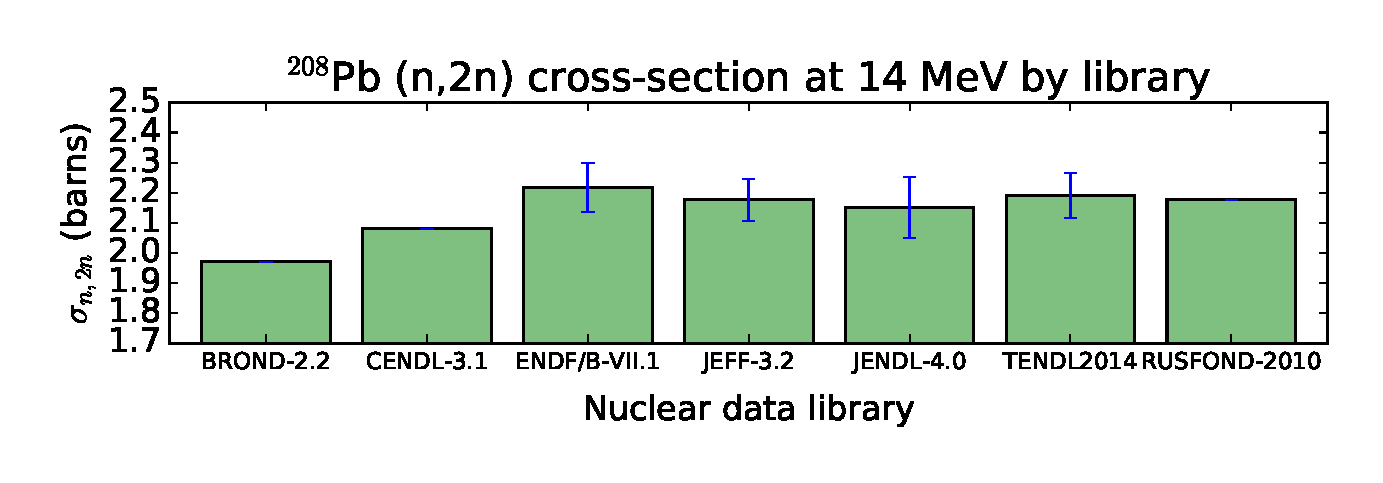
\includegraphics[width=0.47\textwidth]{pb208_n2n_by_lib}
%   \caption{$^{208}$Pb(n,2n)$^{207}$Pb cross-sections at 14MeV with their associated uncertainties for various libraries.}
%   \label{fig:lead_by_library}
% \end{figure}

% Read through section, decide on underlying topics
% Generate sub headings 
% Find papers
% Summarise and write

% HEADINGS
% Uncertainty propagation (see Michael Rising)
%   ? Conventional ?
%   Total Monte Carlo
% Uncertainty in fusion relevant nuclear data
%   Example - DT cross-section?
%   Example - Be multiplicity? O-16 scatter?
%   Example - Lead multiplicity
% END HEADINGS

\FloatBarrier
\subsection{Uncertainty propagation}
% Rising pg 90, ref 83,84
Those in the nuclear engineering field who use nuclear data (ND) are concerned with how `integral' quantities such as heating rates, neutron fluences, TBRs, etc. are impacted by ND uncertainties. To estimate this, one must `propagate' the uncertainty from data to integral quantities. The main approaches are perturbation theory / sensitivity analysis and sampling methods. Perturbatory approaches were developed first and applied with great effect to fission reactor systems. Sampling methods only became available with the increases in computing power achieved in the 21\textsuperscript{st} century. The basics of the methods and the merits and demerits of each are described below.

\FloatBarrier
\subsubsection{Perturbation and sensitivity}
\label{subsubsec:pert}
Perturbation theory is widely applied in many branches of the sciences, and generally consists of substituting an unsoluble equation for a related, soluble one plus some perturbatory series of terms. These increasing order terms have less and less impact on the result and the series is truncated at some point. 

Work on applying this approach to reactor physics problems was undertaken by Wigner on the first nuclear pile \cite{Rising2012}. A more sophisticated framework was developed by Gandini, the Generalised Perturbation Theory (GPT) \cite{Gandini1967} and subsequently into the Equivalent Generalised Perturbation Theory (EGPT) \cite{Gandini1986}. These efforts require obtaining the forward and adjoint solutions to the Boltzmann transport equation such that one can identify the magnitude of responses to any input perturbation. This means GPT and EGPT naturally lend themselves to deterministic methods for radiation transport, where full solutions to the Boltzmann equation are obtained, rather than a subsection of its phase space sampled (as in stochastic methods). This was overcome relatively recently for fission with codes like TSUNAMI-3D by Rearden, which can calculate uncertainties in $k_{\mathrm{eff}}$ with deterministic or Monte Carlo methods \cite{Rearden2004}. An alternative method, not specific to fission problems, is to couple a radiation transport code such as MCNP \cite{Goorley2012} with the SUSD or SUS-3D codes \cite{Kodeli2001}. MCNP is used with perturbed cross-sections to determine how sensitive, $S$, a response parameter, $R$, is to changes, $\delta \sigma_{g}$, in a cross-section group, $\sigma_{g}$, as shown in equation~\ref{eq:sensitivity}. 

\begin{equation}
  \label{eq:sensitivity}
  S = \frac{(\delta R)/R}{(\delta \sigma_{g}) / \sigma_{g}}
\end{equation}

SUS-3D can be used to combine processed covariance information with these sensitivity profiles to determine the uncertainty in various response parameters. Further detail on perturbation theory applied to radiation transport systems can be found in \cite{Sabouri2013}.

A disadvantage of perturbation theory methods is that they embody a linear relationship between input and output uncertainty (see equation~\ref{eq:sensitivity}). Also, covariance matrices are based on normally distributed uncertainties, whether or not this is in reality the case. The method is very much dependent on the quality and comprehensiveness of covariance matrices available. Very large and difficult to compile covariances matrices are required to record the potential correlations between all open reaction channels. 

\nomenclature[z]{GPT}{Generalised Perturbation Theory} 
\nomenclature[z]{EGPT}{Equivalent Generalised Perturbation Theory} 
\nomenclature[z]{TSUNAMI-3D}{Tools for Sensitivty and Uncertainty Analysis Methodology Implementation in three Dimensions}

\FloatBarrier
\subsubsection{Sampling}
\label{subsubsec:tmc}
A variety of sampling based techniques for propagating nuclear data uncertainty are available.

Koning and Rochman developed a new, integrated method of uncertainty propagation in the late 2000s \cite{Koning2008}. This approach, known as Total Monte Carlo (TMC), relies on repeated sampling of varied nuclear data. Whichever problem is being investigated is simulated multiple times with different data, building a distribution of outcomes. It is a fundamentally different method to the sensitivity / perturbation approach. 

The foundation is a reliable methodology for generating nuclear interaction data. The software package T6 \cite{Koning2005} collects together various tools for calculating, formatting and validating nuclear data. Using T6 and a set of input parameters, reaction likelihoods and outcomes can be simulated for a variety of incident particles: neutron, photons, protons, deuterons, tritons helions and alpha-particles and for a range of energies from $10^{-5}\mathrm{eV}$ to $200\mathrm{MeV}$. The interactions in the 1 keV -- 200 MeV incident energy range are computed with the TALYS component of T6. This includes the optical model, level densities, direct reactions, compound reactions, pre-equilibrium reactions and fission reactions \cite{TALYS2017}.

The theoretical models require parameters which may be directly experimentally measured, or are estimated through fitting to other, robust experimental data such as total cross-sections, $\sigma_{t}$. The RIPL-3 nuclear parameter database \cite{Capote2009} contains reference values and confidence estimates for many of these parameters. These and other sources have been assimilated and parsed to provide default values for TALYS, with variances. 

\begin{figure}
  \centering
  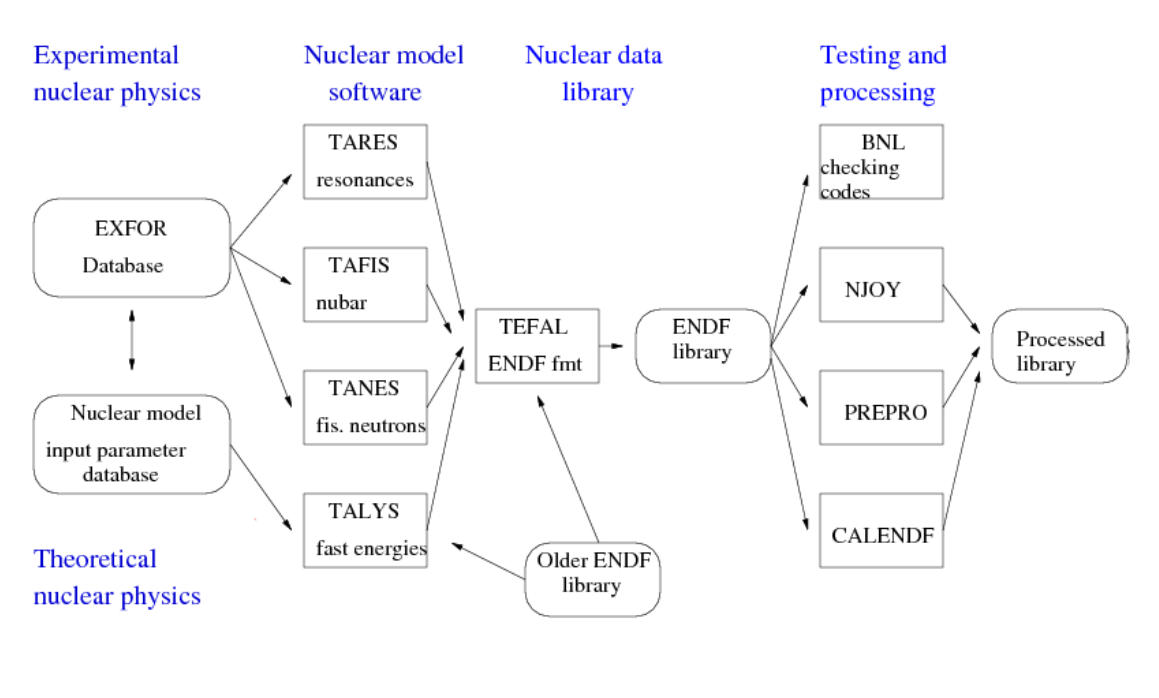
\includegraphics[width=\textwidth]{t6_flow.png}
  \caption[Nuclear data generation in T6 package.]{Nuclear data generation flowchart for the T6 software package. Figure from \cite{Koning2013}.}
  \label{fig:t6_overview}
\end{figure}

A set of nuclear parameters, $\vec{A} = [A_{1},\ldots,A_{n}]$, are used as input to T6 to generate a complete ND library, with full cross-section, resonance, angular distribution, double-differential distribution, covariance, etc. information. These data are self-consistent. An example of this behaviour is where a total cross-section is well understood, it is to be expected that a reduction in one reaction channel cross-section, say elastic scattering, would correspond with an increase in another open reaction channel. This correlation can be produced with simple adjustment or perturbatory approaches but it requires sufficient covariance information, which is often lacking. Once the ND have been generated they are processed and formatted to the ENDF standard with the TEFAL component of the T6 package, permitting use by all ENDF compliant codes \cite{Koning2012}. The ND generation process is shown as figure~\ref{fig:t6_overview}.

Using the above nuclear physics parameter database and models, it is possible to repeat the nuclear data generation process to create a `library of libraries', implicitly containing amongst their variance the uncertainty in the underlying nuclear physics parameters, $\vec{A}$. This data is now used as input to whichever nuclear system is to be simulated. Numerous simulations are launched, each picking a new set of input data, an evaluation from the library of libraries. Whichever reaction rates or spectral quantities can be tallied for inspection and subsequent analysis. Call the quantity of interest $q$. As the number of simulations, $n$, increases, any histogram of the values of $\vec{q} = [q_{1},\ldots,q_{n}]$ will converge to a probability distribution function of the most likely value and its associated uncertainty, $\sigma_{observed}$. 

In an ideal case, this observed uncertainty, $\sigma_{observed}^{2}$, would all be due to the variations in nuclear data, $\sigma_{A}^{2}$, as in equation~\ref{eq:det_variance_sum}.

\begin{equation}
  \label{eq:det_variance_sum}
  \sigma_{observed}^{2} = \sigma_{A}^{2} 
\end{equation}

Indeed this is the case for deterministic methods. With Monte Carlo methods however, answers are inherently uncertain. Rather than solving an equation to find the exact flux and associated reaction rates at every point, the system behaviour is sampled by virtual particles (see section~\ref{sec:radiation_transport} in chapter~\ref{chap:introduction}). Monte Carlo methods depend on the Law of Large Numbers (LLN), using a large number of simulated particles to converge on some mean behaviour. Far fewer particles populate the simulation than the real system. Short of an infinite number of `source' particles, there is always an associated uncertainty. 

Therefore, in this work the observed uncertainty, $\sigma_{observed,i}$ from a simulation $i$ is composed of two components: uncertainty from the simulation method, the standard deviation $\sigma_{stat.,i}$ and uncertainty from the nuclear data, the standard deviation being $\sigma_{A,i}$. So long as these are independent, their variances sum to give the total variance, as in equation~\ref{eq:variance_sum}.

\begin{equation}
  \label{eq:variance_sum}
  \sigma_{observed,i}^{2} = \sigma_{A,i}^{2} + \sigma_{stat.,i}^{2}
\end{equation}

Assembling a histogram of the simulated values, $\vec{q}$, approximates the underlying PDF of the quantity, $q$ of interest. We can modify equation~\ref{eq:variance_sum} from the single simulation case to extract information on the nuclear data uncertainty contained within the PDF of all simulations. The average statistical standard deviation, $\overline{\sigma}_{stat.}^{2}$, shown in equation~\ref{eq:average_stat} is simply the mean value from all $n$ simulations. Substituting this for $\sigma_{stat.,i}$ we have equation~\ref{eq:average_variance_sum}. 

\begin{equation}
  \label{eq:average_stat}
  \overline{\sigma}_{stat.}^{2} = \frac{1}{n} \sum^{n}_{i=1}\sigma^{2}_{stat.,i}
\end{equation}

\begin{equation}
  \label{eq:average_variance_sum}
  \sigma_{observed}^{2} \approx \sigma_{A}^{2} + \overline{\sigma}_{stat.}^{2}
\end{equation}

If the variance due to nuclear data, $\sigma_{A}^{2}$, is to be known, one must either enforce $\overline{\sigma}_{stat.}^{2} = 0$, or otherwise find the difference between the observed and `statistical' simulation variance. 

In terms of determining this statistical simulation uncertainty, Monte Carlo codes provide an estimate of $\sigma_{stat.,i}$. Comparing this uncertainty amongst differing values of $q$ can be achieved by normalising by $q$. The Relative Standard Deviation (RSD)\footnote{Also known as the Fractional Standard Deviation (FSD)}, $R$, is given below as equation~\ref{eq:rsd} and its functional dependence on particle count as equation~\ref{eq:rsd_m}.

\begin{equation}
  \label{eq:rsd}
  R = \frac{\sigma_{stat.}}{q}
\end{equation}

\begin{equation}
  \label{eq:rsd_m}
  R \propto \frac{1}{\sqrt{m}}
\end{equation}

Where $q$ is the reported quantity mean value and $m$ is the simulation particle population count. Keeping $R$ to an arbitrarily small value, say <0.005, allows us to ignore the $\overline{\sigma}_{stat.}^{2}$ term in equation~\ref{eq:average_variance_sum} \cite{Rochman2014a}.

If only one nuclear parameter, $A_{i}$, is varied then the nuclear data uncertainty, $\sigma_{A}$ is wholly attributable to that parameter. Similarly, if only one nuclide has its nuclear parameters and hence interaction data varied, $\sigma_{A}$ represents uncertainty on $q$ from that nuclide alone. When more parameters are varied for more nuclides, the uncertainty is an ensemble of their variation. 

\nomenclature[z]{RSD}{Relative Standard Deviation}
\nomenclature[z]{LLN}{Law of Large Numbers}

The general TMC process is diagrammatically outlined in figure~\ref{fig:tmc_overview}. Compared to other methods, this approach has a variety of benefits. One advantage of this system is that one relates uncertainty in the earliest possible parameters, say the real volume potential or imaginary surface potential of the optical model to the integral quantities of most interest to end-users such as TBR or nuclear heating in a fusion context. This allows future targeting of nuclear physics research--where are resources best allocated to reduce system uncertainties? This is the idea represented by the sensitivity feedback loop in figure~\ref{fig:tmc_overview}. Of course, this methodology does not have to only vary nuclear physics parameters, one can choose to vary parameters in the simulation model, or even methodology, to determine their contribution to uncertainty. Engineering parameters, such as component dimensions, operating temperatures, nuclide atomic densities, etc. can be varied to see how uncertainty on them effects quantities of interest.

\begin{figure}
%  \figuretitle{}
  \centering
  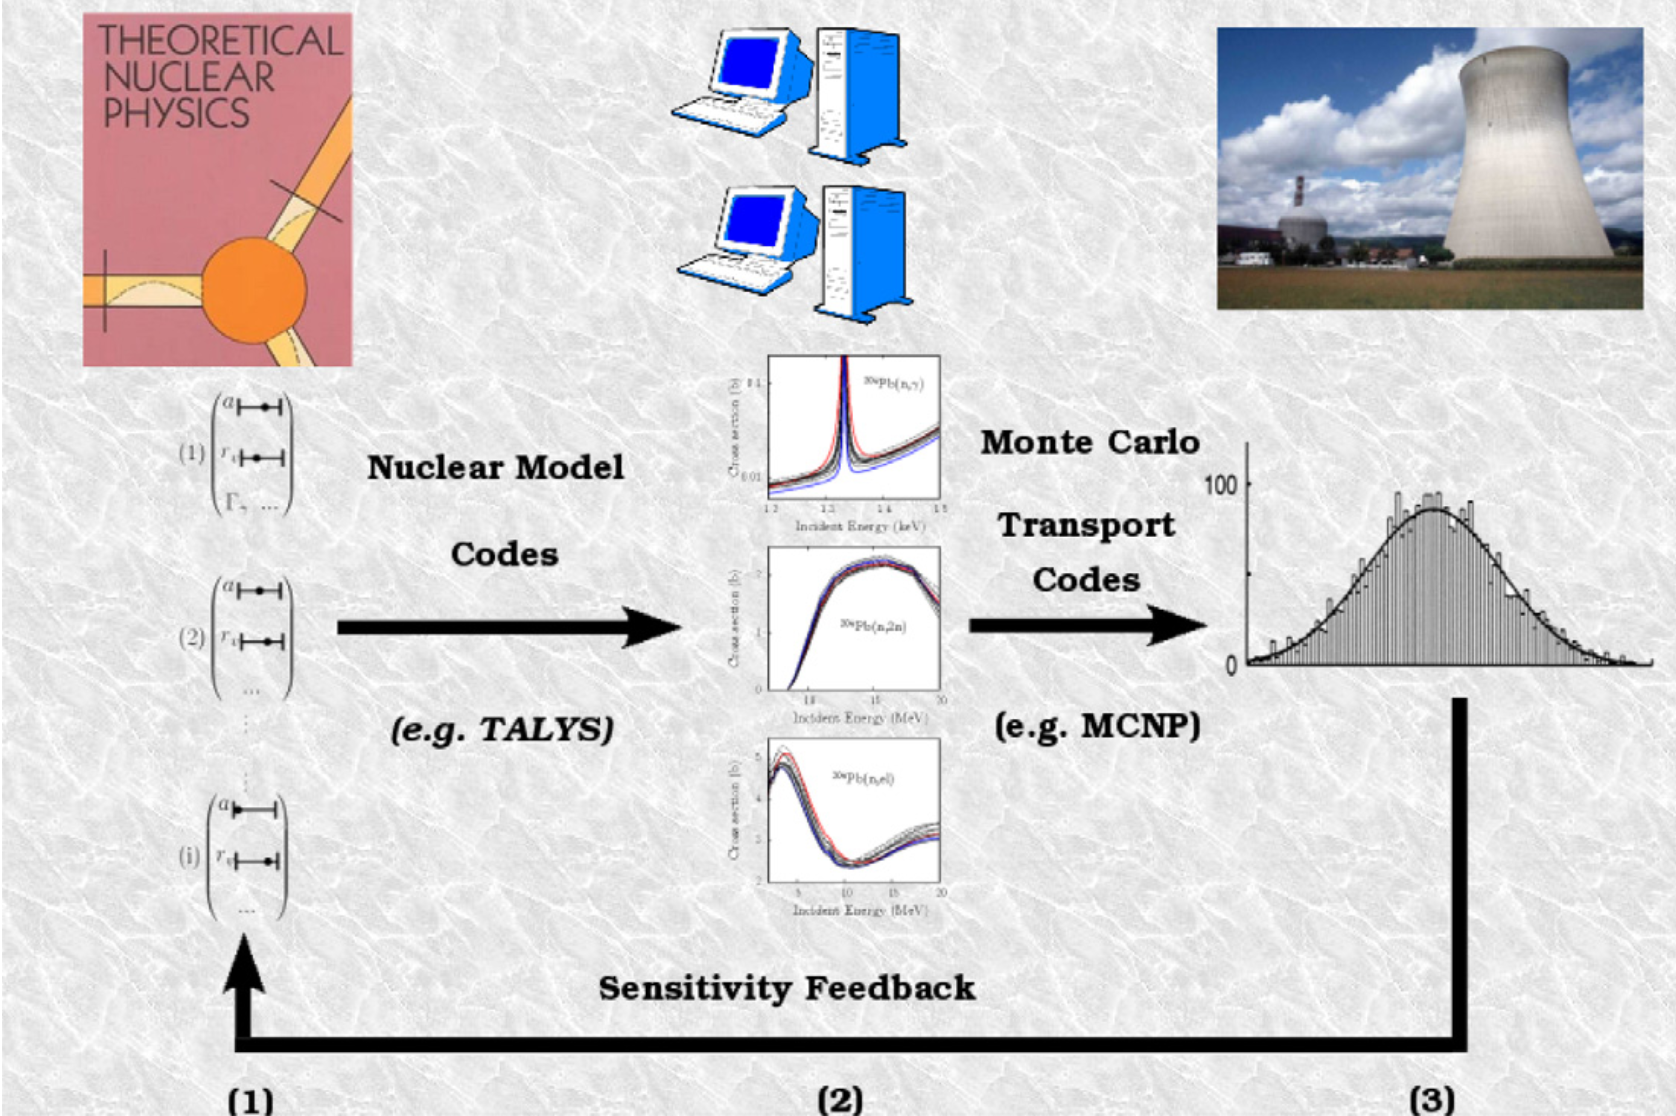
\includegraphics[width=0.8\textwidth]{tmc_overview.png}
  \caption[Total Monte Carlo process schematic.]{Schematic overview of the TMC process. 1) Uncertainties in fundamental nuclear parameters estimated. 2) Many sets of ND generated with T6 software, sampling from fundamental parameters. 3) Nuclear system is simulated many times with generated ND, value of observable is added to PDF, eventually converging on an observable with a mean value and characteristic distribution. Figure from \cite{Koning2008}.}
  \label{fig:tmc_overview}
\end{figure}

Besides TMC, there do exist other sampling based methods. Typically these sample from the uncertainty represented in covariance matrices. For instance, SANDY \cite{Fiorito2017} and NUSS \cite{Zhu2015}. SANDY is a program written in Python which can read ENDF-6 formatted nuclear data files, extract variance-covariance information as random variables and then use these distributions to create a selection of new nuclear data files which embody the underlying uncertainty. NUSS performs a similar function. These methods can of course use whichever covariances are available to generate their perturbed files. As with TMC they rely on repeating the radiation transport part of any calculation multiple times, and so are less appropriate for the most computationally intensive problems.

\FloatBarrier
\subsubsection{Comparison of methods}
Sections \ref{subsubsec:pert} and \ref{subsubsec:tmc} have discussed the methods of two broad uncertainty propagation schemes. It is worth noting the advantages and disadvantages of each, drawing some comparisons between them to elucidate where each method might be most appropriate.

The perturbation method, using covariance information and sensitivity profiles, has much experience associated with it. It has been used to estimate uncertainties for $k_\mathrm{eff}$ and other important parameters in fission reactor physics for several decades. By contrast, whilst the idea of repeatedly simulating a system with different inputs is not new, the integrated TMC methodology, with a sophisticated ND generation package, is novel. Published in 2008, it has seen substantially less use in industry than perturbatory approaches. The nuclear industry is often slow to adopt new technology as there can be a significant volume of work required to validate results, especially where their application is safety-critical. Studies in a variety of applications have sought to benchmark and demonstrate TMC, bringing it into wider use \cite{Koning2008}\cite{Rochman2010}\cite{Sjostrand2017}\cite{Koning2012}\cite{Alhassan2014}\cite{Alhassan2015a}\cite{Rochman2011a}. 

Assuming appropriate nuclear data is already available, the slowest component of either method is radiation transport by some Monte Carlo code. Combining covariance information with sensitivity profiles, or parsing results from multiple TMC simulations to assemble a PDF of some target quantity, $q$, is of minor computational burden. If the time taken for a single simulation is $T$ time units, then TMC will take $n \times T$ where convergence on some $q$ and its $\overline{\sigma}_{observed}$ typically takes $n \geq 500$ simulations to sufficiently sample input uncertainties \cite{Rochman2014a}. This factor of several hundred slowdown is clearly a burden for many analyses, especially those requiring many billions of source particles such as full-core fission reactor simulations, shielding analyses or similar. 

In the past 3 or 4 years, progress has been made in reducing the TMC time penalty. If a single calculation requires $m$ particles for convergence, so-called `Fast TMC' uses $m/n$ particles in each of the $n$ simulations. This dedicates fewer particle histories to each change in nuclear data, exploring the $A$ parameter-space more quickly, but with a larger $\sigma_{stat.}$ for each simulation. \citeauthor{Rochman2014a} indicate that ensuring the inequality $\frac{\sigma_{stat.}}{\sigma_{observed}} \leq 0.5$ holds for each simulation, equation~\ref{eq:average_variance_sum} is still valid and the scheme still computes approximately the same uncertainties as $n$ runs each with $m$ particles. This is in contrast to traditional TMC where the rule of thumb is $\frac{\sigma_{stat.}}{\sigma_{observed}} \leq 0.05$.

Perturbatory methods require covariance matrices, but often only covariance information for certain phenomena are readily available. Along with cross-sections and resonance parameters there are angular distributions of scattered and emitted particles, double-differential distributions, $\overline{\nu}$ (average neutron yield from a fission event), etc. Evaluations vary in their completeness. As TMC calculates and varies a full complement of nuclear data with its set of nuclear models, it can claim to have a more comprehensive estimate of the true uncertainty. While perturbations to generate sensitivity profiles are for a single cross-section group value (for example), TMC varies parameters at an earlier step, as a fundamental parameter for the behaviour of the nucleus. Because of this, when a parameter is varied in the TMC approach, it in turns varies all correlated phenomena. Other areas where the TMC scheme embodies a more complex approach are the assumed linearity of the perturbation method, along with the inability of perturbation methods to accommodate non-Gaussian observable distributions. Despite these advantages, the TMC method has attracted certain criticisms. It can be argued that the all-important nuclear parameter distributions have not been rigorously estimated from experimental data \cite{Helgesson2017}. Both \citeauthor{Capote2010} and \citeauthor{Rising2012} note the arbitrariness of some parameter distributions. Recently, work has been undertaken to implement Bayes' theorem through the assignment of weights to generated ND \cite{Koning2015a}.

% ENDF-6 does not support covariances for some kinds of data, such as double-differential data \cite{ENDF-6}. 

The ease of application of the two methods is varied. While TMC is conceptually easy to understand and incorporates many advantageous features, there are limitations in its application currently, such the failure of TALYS to correctly predict the behaviour of light nuclides (the cut-off being A=12) \cite{Rochman2011}. For perturbation methods, the paucity of covariance information is a problem for some calculations (principally those outside the thermal fission realm). 

\FloatBarrier
\subsection{Uncertainty in fusion relevant data}
There are many nuclides of importance in nuclear fusion studies whose behaviour are not known to sufficient accuracy \cite{Forrest2011}. Nuclear technology development programmes for ITER \cite{Batistoni2008} and DEMO \cite{Abdou2015} have both identified the need for more widespread uncertainty estimates and more accurate nuclear data evaluations to reduce uncertainties. \citeauthor{Batistoni2008} cites conservative uncertainties for neutron fluence at the ITER pressure vessel ($\pm 15\%$) and superconducting Toroidal Field (TF) coil magnets ($\pm 30\%$) due to nuclear data uncertainties. 

An improved uncertainty treatment has been advocated for tritium breeding since the early days of detailed reactor design \cite{Abdou1986}. \citeauthor{Youssef1986} performed a sensitivity / perturbation analysis on uncertainties in TBR due to ND for early blanket designs finding that ND contributed an uncertainty on TBR of between 2--6\% of the mean value depending on the specific design. 

A variety of different tritium breeding schemes are proposed for reactors. These have either solid (ceramic pebbles) or liquid (molten metal) breeding compounds which may or may not be accompanied by an additional neutron multiplying material. The solid systems have some sort of additional coolant loop, typically employing He or H\textsubscript{2}O. For the liquid metal systems, the breeder also functions as the primary coolant. All systems are likely to have a secondary coolant loop for subsequent electricity generation. \citeauthor{Youssef1986} compared the TBR uncertainty due to ND for several of these systems. He found that Li\textsubscript{2}O ceramic systems typically have a large uncertainty contribution from \textsuperscript{16}O, followed by \textsuperscript{56}Fe and the lithium isotopes (their relative importance depending on the degree of \textsuperscript{6}Li enrichment). Uncertainty in a LiAlO\textsubscript{2} system on the other hand was dominated by uncertainty in \textsuperscript{9}Be multiplicity cross-section data. As such, there were significant differences between similar breeding concepts, which is a frustration when trying to generalise and also underscores the importance of this kind of work. For a Li-Pb, liquid metal system, the TBR uncertainty was dominated by variance in the lead multiplicity cross-sections, the (n,2n) and to a lesser extent (n,3n) reactions.

As well as pure computation, work is available comparing simulation and experimentally determined values for important reaction reaction channels in ceramic (HCPB) tritium breeding systems \cite{Batistoni2007}. Less work has been undertaken to experimentally corroborate simulated nuclear responses in liquid metal blankets. This is not for lack of desire, these lithium-lead blankets are currently in development in tandem with the solid breeders and account for half of the Test Blanket Modules (TBM) to be tested in ITER \cite{Chuyanov2010}. There are good reasons to expect lithium-lead blankets to be yet further developed, reasons including: the greater resource availability (beryllium for ceramic blankets is in limited supply \cite{Bradshaw2011} \cite{Shimwell2014}), the facility for on-load lithium enrichment and thus TBR adjustment \cite{Ihli2008}, higher natural breeding ability \cite{Colling2012} and the comparative ease of extracting bred tritium from a liquid metal vs. porous pebbles. A more thorough discussion on the advantages and disadvantages of the different technologies can be found in \cite{Abdou2015}. Given the above, it is worth investigating the impact of ND uncertainties on LiPb type blankets.

%\nomenclature[z]{HCPB}{Helium Cooled Pebble Bed}
%\nomenclature[z]{HCLL}{Helium Cooled Lithium Lead}
\nomenclature[z]{TBM}{Test Blanket Module}
\nomenclature[z]{TF}{Toroidal Field}

% The other examples seem strange to include if there's not going to be any TMC analysis...
%\subsubsection{Deuterium-Tritium}
%\subsubsection{\textsuperscript{16}O scattering}
%\subsubsection{Lead multiplicity}

As briefly mentioned previously, \citeauthor{Leichtle2011} has undertaken a recent study where nuclear data was adjusted to obtain the sensitivity of TBR in a modern HCLL system (the ITER HCLL TBM) to various nuclear reaction cross-sections \cite{Leichtle2011}. This work identified $^{6}$Li, $^{56}$Fe and the Pb cross-sections as the most important for TBR uncertainty from the a ND perspective. The analysis below looks at variation in lead nuclear data. 

\FloatBarrier
%\subsection{DEMO}
% Should this be here? Perhaps it doesn't need a whole bit...

\FloatBarrier
\section{Method}
This chapter is investigating the propagation of lead nuclear data uncertainties to a corresponding PDF for TBR uncertainty in the DEMO reactor. The following section describes nuclear data selection and sampling, along with radiation transport and data analysis methods for the study.

\subsection{Nuclear data}
\label{subsec:data}
As discussed in section~\ref{subsubsec:tmc}, traditionally cross-section uncertainties are represented as single values for a given energy and reaction channel. There might be an estimate of uncertainty, which is typically given as a 1 $\sigma$, the standard deviation of a Gaussian distribution centred about the quoted mean value. As an example, the $^{208}$Pb(n,2n)$^{207}$Pb neutron multiplication reaction at 14 MeV is shown in table~\ref{tab:lead_by_lib} for a variety of experiments and nuclear data libraries. Experimental results from the EXFOR library are also shown. There are a wide spread of experimental results, for example Arakita and Shunk are relatively low at 1.04 and 1.31 b respectively and with quoted uncertainties of 5.77 and 8.0\% respectively. These values are among the older data experimental data and have been relegated in importance by nuclear evaluators. Modern evaluated data releases tend to agree on a figure of $\sigma_{n,2n}(14\ \mathrm{MeV}) \approx 2.1$ barns. It would appear that the experiments of Simakov and Frehaut along with model calculations have been favoured of to produce the data contained within contemporary evaluated nuclear data libraries. Data shown in table~\ref{tab:lead_by_lib} are also shown graphically in figure~\ref{fig:tendl_lead} along with the 300 TENDL files used for this work.

\begin{table}[H]
  \footnotesize
  \centering
  \begin{tabularx}{\textwidth}{XXXX}
    \toprule
    Source & Energy [MeV] & $\sigma_{n,2n}$ [b] & $\pm\%\Delta\sigma_{n,2n}$ \\
    \midrule
    Experimental data &      &      &    \\
    \midrule
    Ngoc & 14.6 & 1.27 & 7.61 \\
    Simakov & 14.1 & 2.38 & 5.88 \\
    Anders & 14.6 & 1.36 & 4.98 \\
    Arakita & 14.2 & 1.04 & 5.77 \\
    Frehaut & 13.8 & 1.96 & 8.11 \\
    Frehaut & 14.3 & 1.94 & 8.36 \\
    Frehaut & 14.8 & 1.97 & 8.52 \\
    Salaita & 14.8 & 1.31 & 8.85 \\
    Shunk & 14.0 & 1.31 & 8.00 \\
    Prasad & 14.8 & 0.99 & 12.12 \\
    Garg & 14.7 & 1.09 & 6.78 \\
    Glagolev & 14.7 & 1.70 & 17.65 \\
    Amemiya & 14.8 & 1.22 & 8.20 \\
    \midrule
    Evaluated data &      &      &    \\
    \midrule
    BROND 3.1 & 14.0 & 2.09 & - \\
    CENDL 3.1 & 14.0 & 2.08 & - \\
    ENDF/B-VII.1 & 14.0 & 2.22 & 8.15 \\
    JEFF 3.2 & 14.0 & 2.18 & 7.0 \\
    JENDL 4.0 & 14.0 & 2.15 & 10.1 \\
    TENDL 2015 & 14.0 & 2.19 & 7.4 \\
    RUSFOND 2010 & 14.0 & 2.18 & - \\
    \bottomrule
  \end{tabularx}
  \caption[Cross-section and uncertainty data for the $^{208}$Pb(n,2n)$^{207}$Pb reaction.]{Cross-section values for the n,2n reaction channel, $\sigma_{n,2n}$ on $^{208}$Pb, around 14 MeV for various experiments and libraries. The experimental results were retrieved from the online EXFOR database \cite{exfor2017}. The ENDF utility code Inter \cite{Dunford2002} was used to extract the values for each library. The uncertainties, $\Delta\sigma_{n,2n}$ are presented as percentages above and below the reported value.}
  \label{tab:lead_by_lib}
\end{table}

% \begin{figure}[H]
%   \centering
% %  \figuretitle{}
%   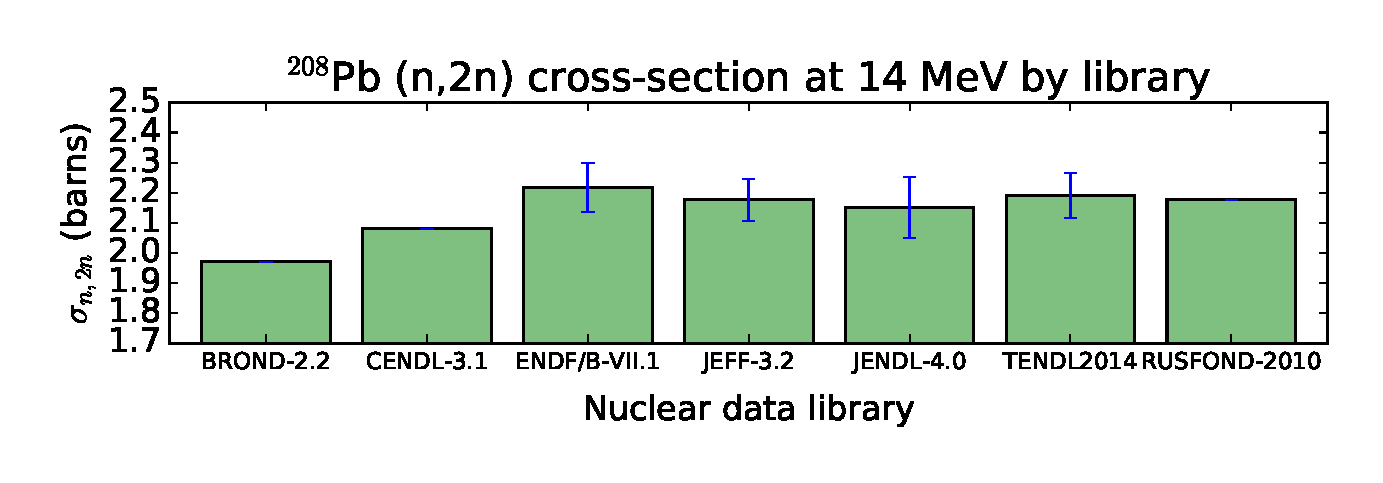
\includegraphics[width=\textwidth]{pb208_n2n_by_lib}
%   \caption{Comparison of (n,2n) cross-section values in major ND libraries for the most abundant lead isotope, $^{208}$Pb. Uncertainties are shown where available.}
%   \label{fig:lead_by_lib}
% \end{figure}

This study used the TENDL-2015 library. It is a comprehensive, general-purpose nuclear data library which contains data on interactions between 7 projectiles and over 2,800 target nuclides. As described above, the library is produced by a suite of codes known as T6 and an adherence to a strict methodology of reproducability \cite{Rochman2016}. It uses the TALYS nuclear reaction code to model high-energy reactions, with TARES handling the lower energy, resonant region. The inputs are fundamental parameters, including data from the RIPL-3 database \cite{Capote2009}, each with their own probability distributions that reflect their uncertainties. The TENDL-2015 release contains `average' or best-guess evaluations, but also a collection of `random' files, those generated using the sampling method. These have been pre-generated by the TENDL team. Comprehensive information concerning the input parameters and plots of the ND are available online \cite{TENDL2015}.

It is instructive to inspect the nuclear data used as input for this TMC simulation. The sampled nuclear data files were downloaded in both ACE (293K) and ENDF format from the TENDL-2015 website \cite{TENDL2015}. Figure~\ref{fig:tendl_lead} shows the (n,2n) cross-sections as a function of energy for $^{208}$Pb. Cross-sections from a given file at a certain energy are shown as grey circles. The mean value of the random files and a standard deviation is also shown, along with available EXFOR data. The shape of this endothermic multiplication reaction is visible, with an energy threshold of 7.36 MeV. The cross-section rises to approximately 2 b in the 14 MeV fusion neutron energy range before falling away at higher energies--here the n,3n reaction becomes more probable. No experimental data is available from the EXFOR database beyond 14.8 MeV. This lack of higher energy information means constraining model parameters for T6 data generation is more difficult and so the uncertainties here are larger.

% \begin{figure}
% %  \figuretitle{}
%   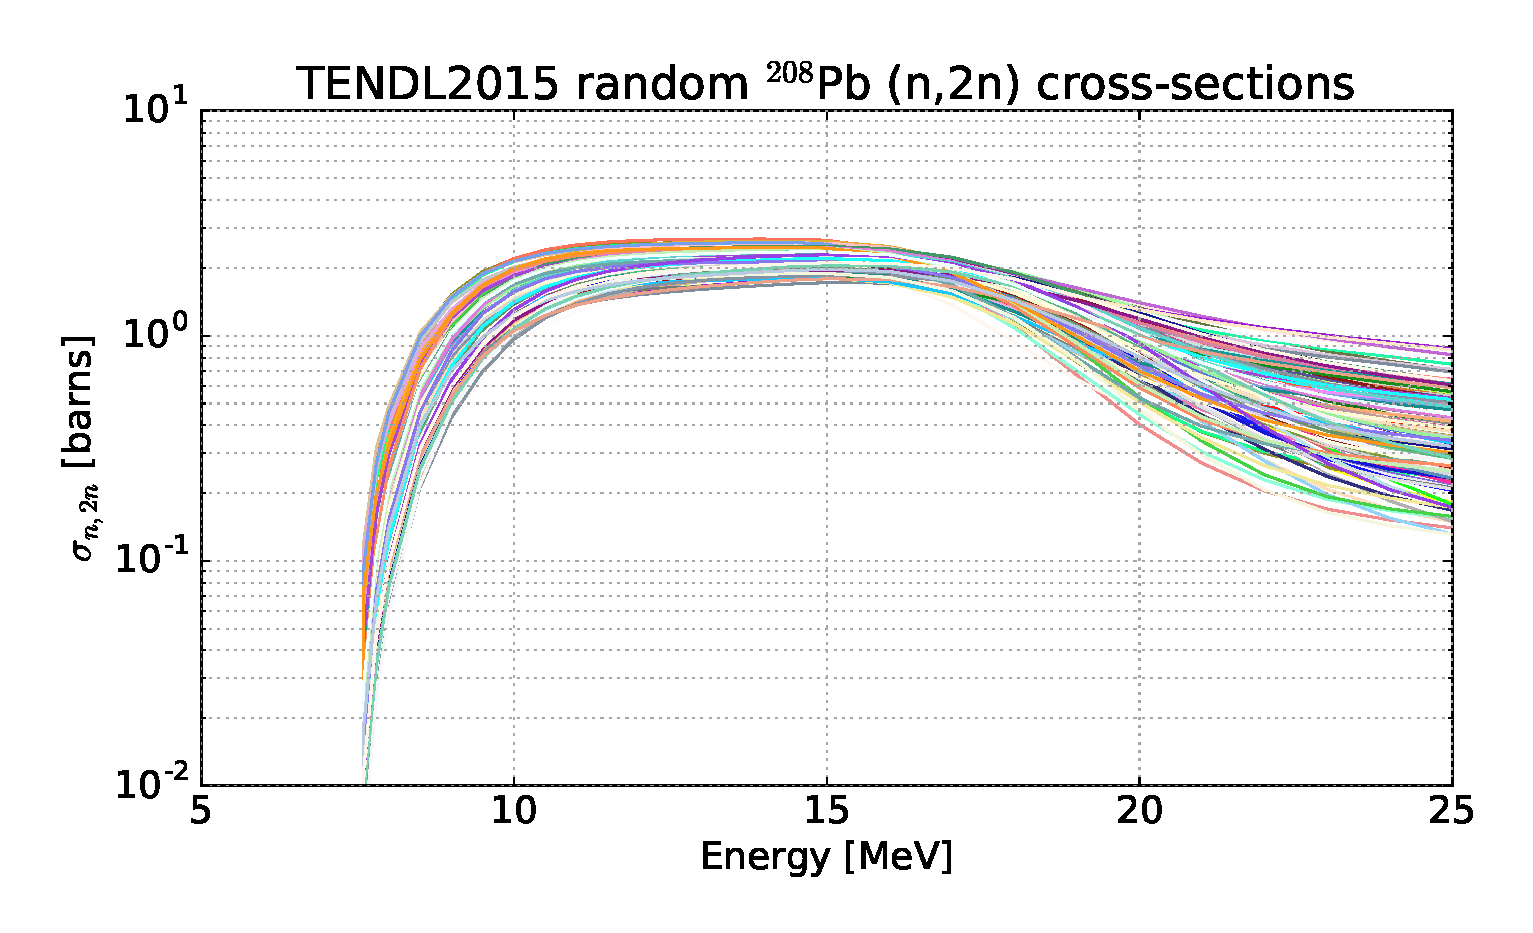
\includegraphics[width=0.48\textwidth]{pb208_tendl_n2n}
%   \caption{Shown here are 300 `random' TENDL2015 n,2n cross-sections as a function of energy for the most abundant lead isotope, $^{208}$Pb.}
%   \label{fig:tendl_lead}
% \end{figure}

\begin{figure}[H]
%  \figuretitle{}
  \centering
  \makebox[\textwidth][c]{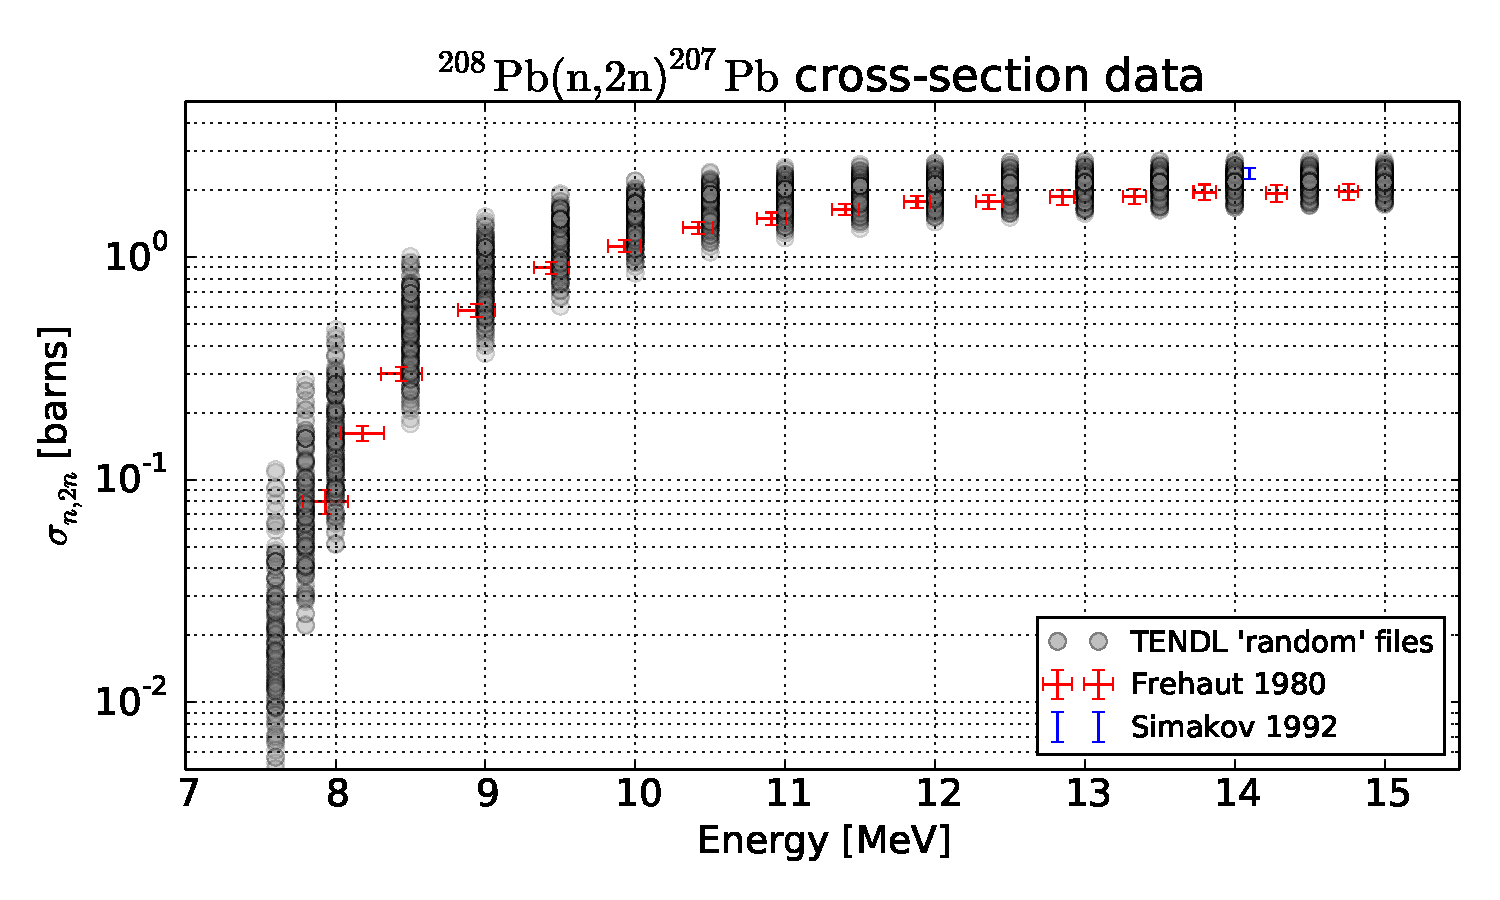
\includegraphics[width=1.1\textwidth]{pb208_n2n_tendl_exfor}}
  \caption[Cross-section and uncertainty data for the $^{208}$Pb(n,2n)$^{207}$Pb reaction.]{Shown here are $^{208}$Pb(n,2n)$^{207}$Pb cross-sections as a function of energy. The plot shows the TENDL `random' data extracted from processed ACE files. Additionally, the few available experimental results in EXFOR are plotted for comparison. The relative paucity of experimental data is one reason for the relatively large uncertainty on this particular reaction channel.}
  \label{fig:tendl_lead}
\end{figure}

In an unmoderated fusion neutron spectrum the dominant reaction channels for Pb are neutron multiplication (n,2n) and elastic scattering, at approximately 2 and 3 barns respectively. The ENDF utility code Inter was used to extract cross-section values at a given energy from the ENDF files. The resulting distributions and correlations were plotted as figures \ref{fig:tendl_n2n}, \ref{fig:tendl_nel} \& \ref{fig:pb_el_n2n_corr}. Figures \ref{fig:tendl_n2n} and \ref{fig:tendl_nel} were examined for their first 3 statistical moments. 

\begin{table}[H]
  \footnotesize
  \centering 
  \begin{tabular}{llll}
    \toprule
    Nuclide & Mean, $\mu$ [b] & RSD, $\frac{\sigma}{\mu}$ & Skewness \\
    \midrule
    Pb206 & 2.11 & 8.1\% & -0.065 \\
    Pb207 & 2.12 & 10.7\% & -0.868 \\
    Pb208 & 2.17 & 9.7\% & -0.120 \\
    \bottomrule
  \end{tabular}
  \caption[Statistical moments of $^{208}$Pb(n,2n)$^{207}$Pb data in TENDL2015.]{TENDL2015 `random' Pb n,2n neutron multiplicity channel cross-section distribution statistics, also shown in figure~\ref{fig:tendl_n2n}.}
  \label{table:n2n}
\end{table}

Figure~\ref{fig:tendl_n2n} and table~\ref{table:n2n} show the distributions of TENDL-2015 cross-sections for (n,2n) at 14 MeV. Lower values for $\sigma_{n,2n}$ will reduce the neutron multiplication of the blanket and, other quantities being equal, result in a reduced total neutron flux and therefore a lower TBR. The first two moments of each distribution in figure~\ref{fig:tendl_n2n} were analysed for convergence testing. A normalised measure of the standard deviation, the relative standard deviation, $R(n) = \frac{\sigma(n)}{\mu(n)}$, where $\sigma(n) = \sqrt{\frac{\sum_{i=0}^{n}(x_{i}-\mu_{i})^{2}}{n-1}}$ and $\mu(n) = \frac{\sum_{i=0}^{n}x_{i}}{n}$ was plotted as a function of sample size. $R(n)$ converges for $n \approx 150$ for both $^{206}$Pb and $^{208}$Pb at 8.1\% and 9.7\% respectively. For $^{207}$Pb, $R(300)=10.7\%$, but this figure is not completely converged, with some step changes in $R$ due to extreme $\sigma_{n,2n}$ cross-sections from the low-value tail. Ideally more data would be available for this nuclide.

\begin{figure}[H]
%  \figuretitle{}
	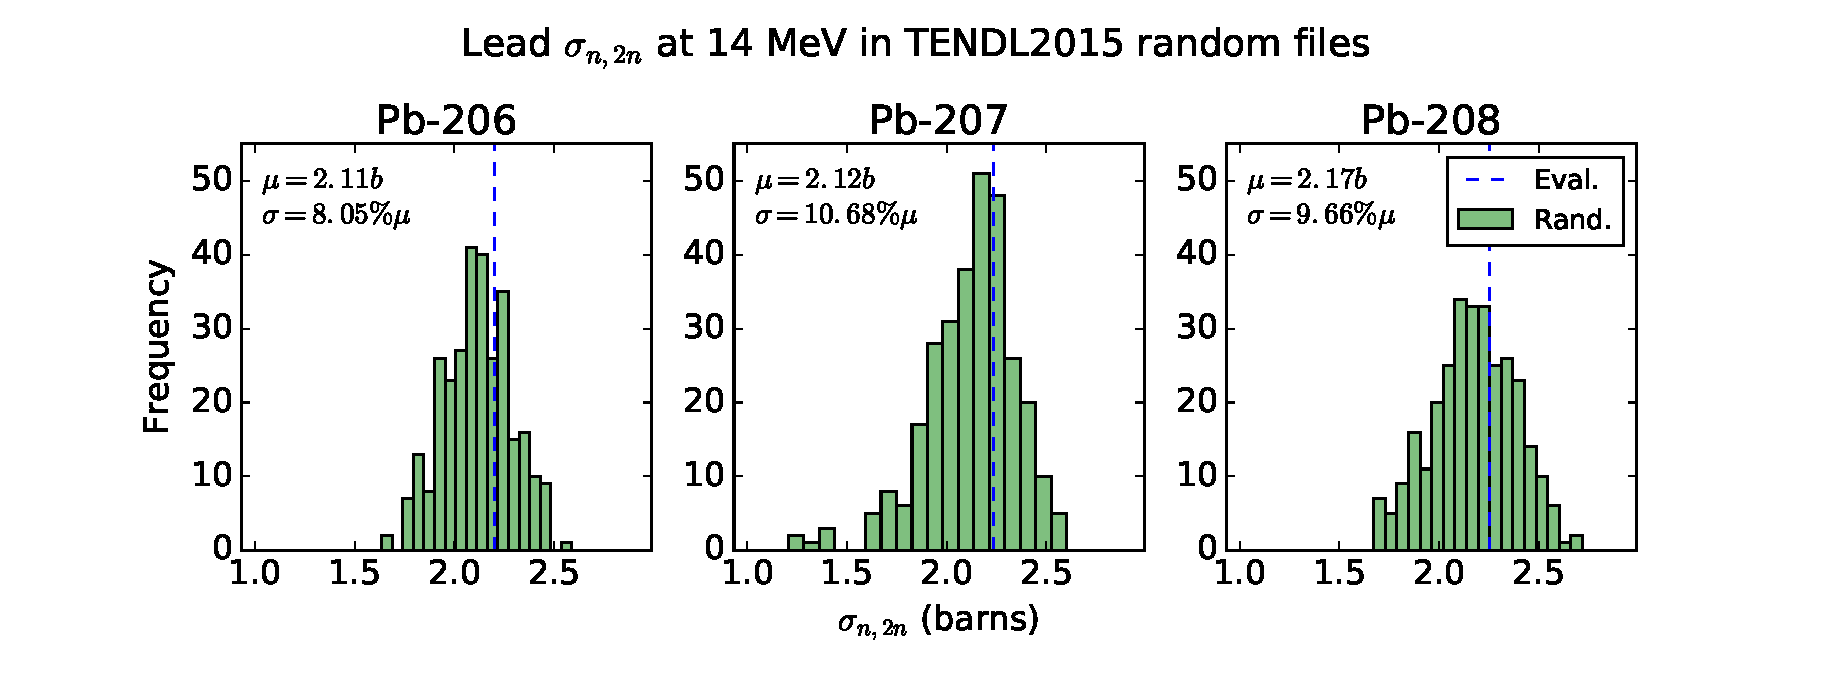
\includegraphics[width=\textwidth]{pb_tendl_n2n_hist}
	\caption[Histograms of $^{208}$Pb(n,2n)$^{207}$Pb data in TENDL2015.]{Shown are histograms of $\sigma_{n,2n}$ at 14 MeV for the three major Pb isotopes. The histogram contains all 300 available files each Pb nuclide. It can be seen that while $^{206,208}$Pb are approximately symmetrical with skewness values close to zero, $^{207}$Pb has a skewness of -0.868 indicating a low-value tail. This may or may not be representative of the underlying distribution.}
	\label{fig:tendl_n2n}
\end{figure}

\begin{table}[H]
  \footnotesize
  \centering 
  \begin{tabular}{llll}
    \toprule
    Nuclide & Mean, $\mu$ [b] & RSD, $\frac{\sigma}{\mu}$ & Skewness \\
    \midrule
    Pb206 & 2.84 & 7.5\% & 0.663 \\
    Pb207 & 2.80 & 8.0\% & 0.548 \\
    Pb208 & 2.81 & 8.1\% & 1.185 \\
    \bottomrule
  \end{tabular}
  \caption[Statistical moments of $^{208}$Pb(n,el)$^{208}$Pb data in TENDL2015.]{TENDL2015 `random' Pb elastic scattering cross-section distribution statistics, also shown as figure~\ref{fig:tendl_nel}.}
  \label{table:nel}
\end{table}

\begin{figure}[H]
%  \figuretitle{}
  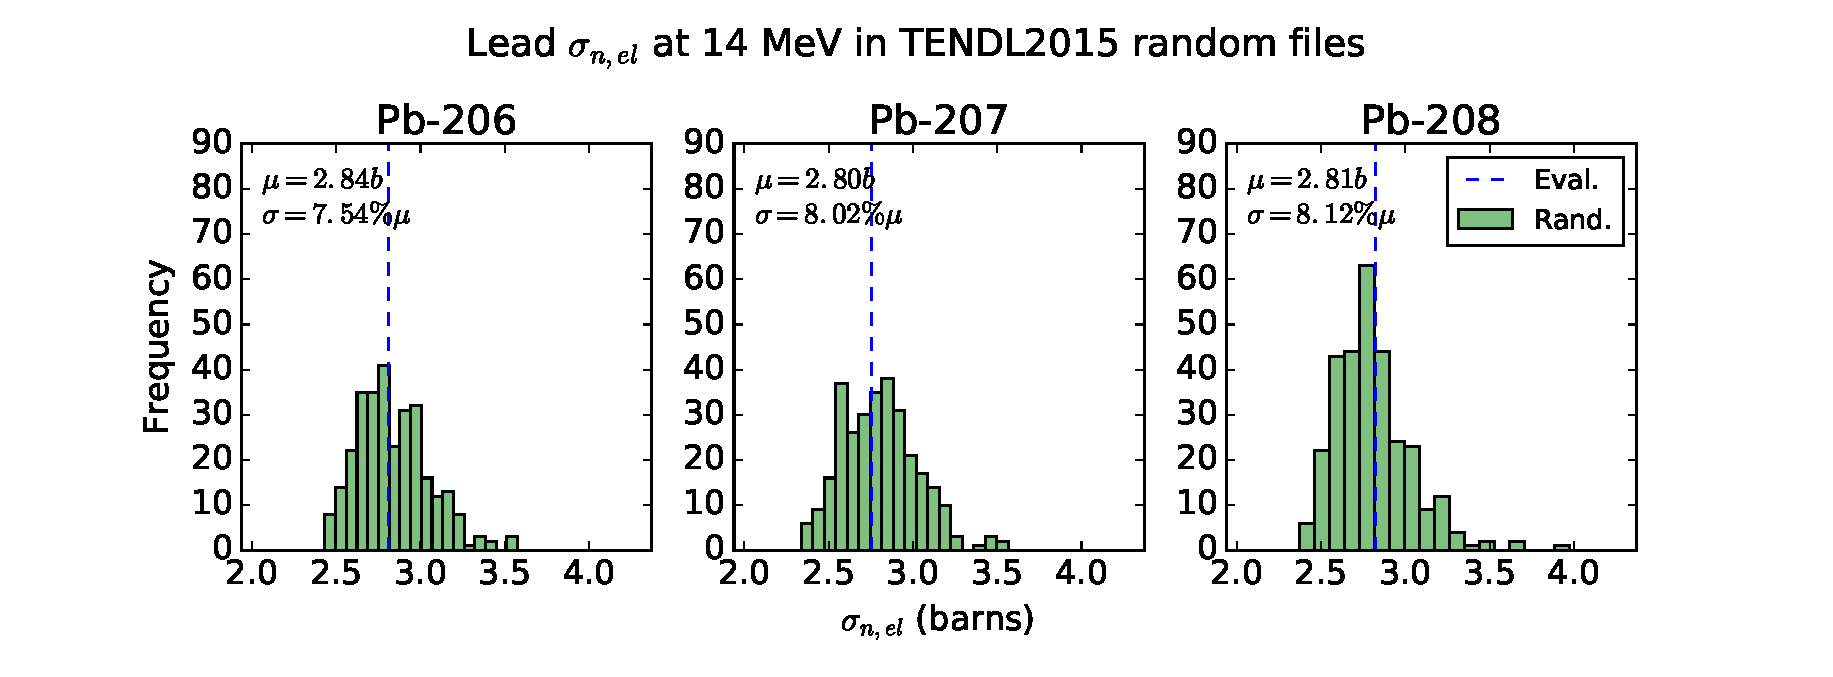
\includegraphics[width=\textwidth]{pb_tendl_nel_hist}
  \caption[Histograms of $^{208}$Pb(n,el)$^{208}$Pb data in TENDL2015.]{The elastic scattering cross-sections for lead at 14MeV are all positively skewed, with $^{208}$Pb having a skewness value of 1.185.}
  \label{fig:tendl_nel}
\end{figure}

The elastic scattering data shown in figure~\ref{fig:tendl_nel} and table~\ref{table:nel} are instead positively skewed, with high value tails for each isotope, with the most pronounced tail being $^{208}$Pb. A greater elastic scattering cross-section will result in an increased likelihood of down-scattering neutrons to lower energies. The softer spectrum will increase triton production in $^{6}$Li as the cross-section increases with decreasing energy, i.e. $\sigma_{n,t}(E) \propto \frac{1}{E}$. However, the elastic scattering cross-section is anti-correlated with the n,2n cross-section in the TENDL data (see figure \ref{fig:pb_el_n2n_corr}). In other words, a high scatter cross-section is typically coupled with a low multiplicity cross-section. This inclusion of cross-channel correlation is one of the key advantages of TMC over more traditional uncertainty propagation (UP) methods. 

% This compensating effect decreases the overall uncertainty where individual perturbations on a single channel would result in an unrealistic, larger uncertainty. 

\begin{figure}[H]
%  \figuretitle{}
	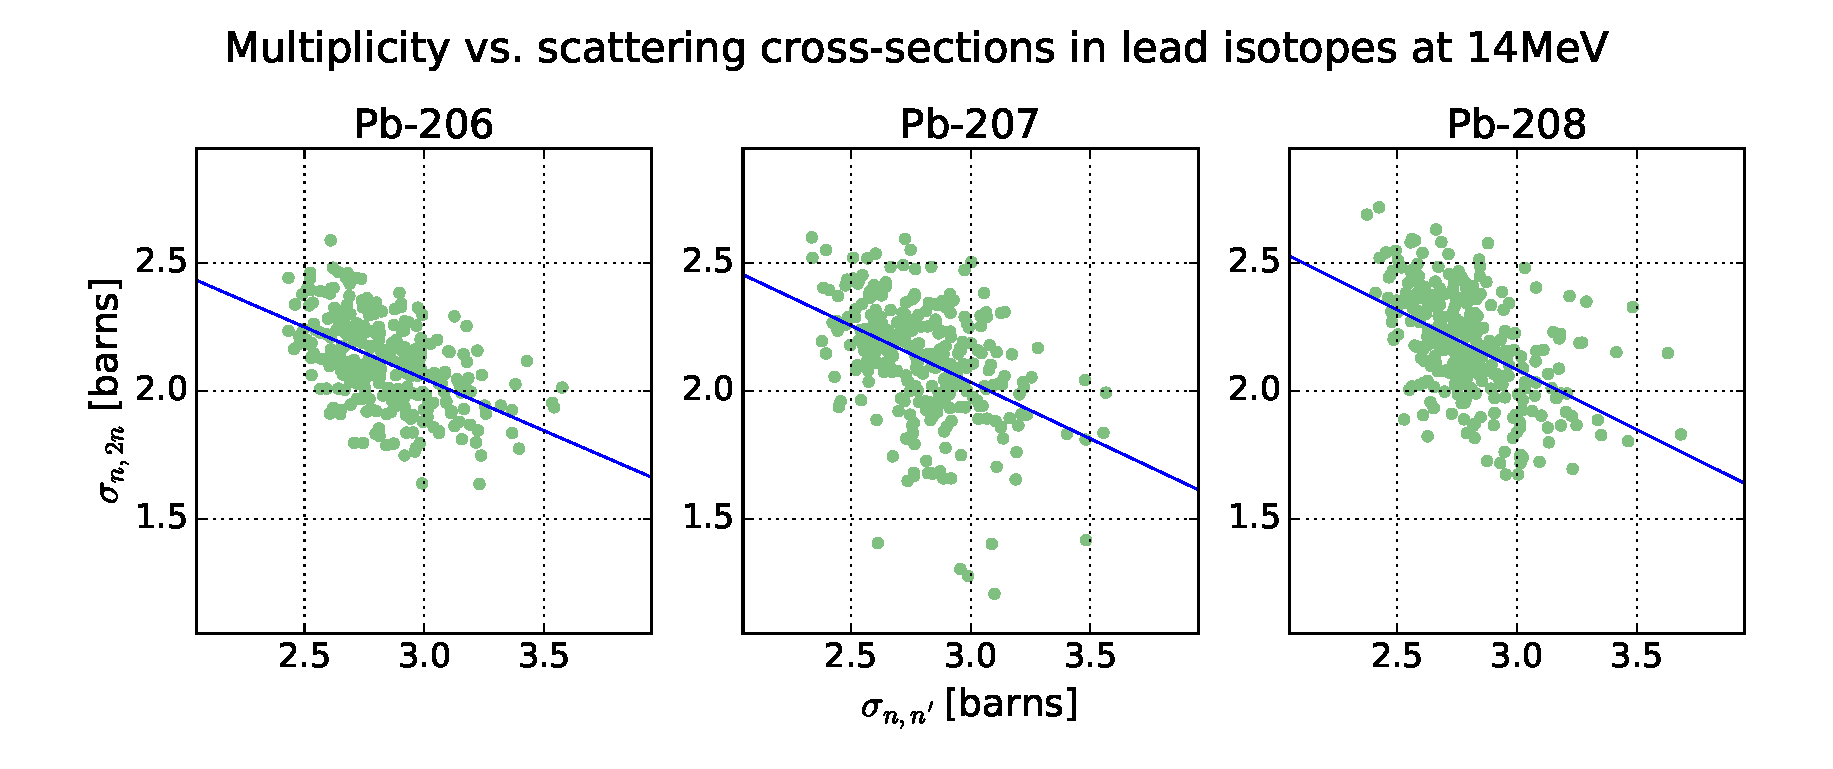
\includegraphics[width=\textwidth]{pb_el_n2n_corr}
  \caption[Correlation between elastic and (n,2n) channels in Pb.]{Shown here are scatter plots of the relationship between the scattering and n,2n cross-sections in the TENDL data. The two channels are clearly anti-correlated. A least squares fit has been applied and the resulting best-fit linear relationship plotted.}
	\label{fig:pb_el_n2n_corr}
\end{figure}

\FloatBarrier
\subsection{Radiation transport}
There exist several variants on the DEMO future fusion reactor concept. It is typically a several GW\textsubscript{th} device, with a major radius, $\mathrm{R}\approx9\mathrm{m}$. Different breeding blanket concepts are the topic of contemporary study and a radiation transport model is typically produced for each one. Of course the nuclear responses within the blanket are of particular interest, but the size and material composition of the blanket also determines the neutron spectra and flux behind them--throughout the rest of the machine.

\begin{figure}[H]
  \centering
	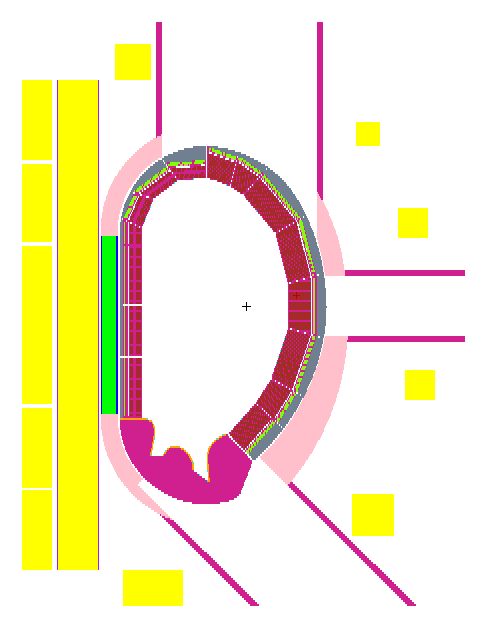
\includegraphics[width=0.5\textwidth]{demo_mcnp}
	\caption[Poloidal slice through DEMO HCLL MCNP model.]{A poloidal slice through the 2014 DEMO HCLL radiation transport model used for this study. Magnets are marked in yellow, the divertor is fuscia and the blanket in red. The blanket sectors are constructed using the MCNP `universe' feature for repeating geometry and do not conform perfectly to the vacuum vessel shape. The three large voids above, below and to the right of the plasma chamber are access ports--extraction routes for blanket and divertor sectors in need of replacement. As noted previously, the distance from the left of this figure to the centre of the plasma chamber is approximately 9m.}
	\label{fig:demo_mcnp}
\end{figure}

An 11.25\degree \ toroidal sector of the 2014 DEMO HCLL MCNP model was modified to tally triton production per source particle (TBR). MCNP6.1 \cite{Goorley2012} was used for particle transport. The particle count for each simulation was set to $3\times10^{6}$ giving a relative standard deviation, RSD on TBR of $\approx 0.002$ for each simulation. This is negligible compared to the total (nuclear data \& statistics) accumulated RSD and so the variance of the observable is assumed to be entirely due to variance in the nuclear data. While other TMC analyses have attempted to limit to the statistical variation to only around half of the total variance and then subtract this from the observable variance, known as `Fast TMC', the original TMC technique of minimising the statistical variance is used here. 

Whilst the Pb nuclear data for sampling was from TENDL-2015, FENDL3.1b data was used for the neutron transport of other elements present in the reactor model. A series of simple Bash and Python scripts were used to sample different \textsuperscript{206}Pb, \textsuperscript{207}Pb \& \textsuperscript{208}Pb TENDL-2015 ACE files for the radiation transport runs, before creating and submitting jobs en masse to the local cluster at the Culham Centre for Fusion Energy. Records of the input ND and tally data were kept, identified by a unique string.

The TMC process was run for a total of 1559 MCNP simulations, each 84 core-minutes across 32 cores. The total wall-clock time was 3 days, 15 hours.

\section{Results \& discussion}
Python scripts were used to plot TBR convergence as a function of simulation count (see figure \ref{fig:convergence}) and the distributions of simulated TBR (see figure \ref{fig:tbr_distribution}).

\begin{figure}[H]
%  \figuretitle{}
  \centering
	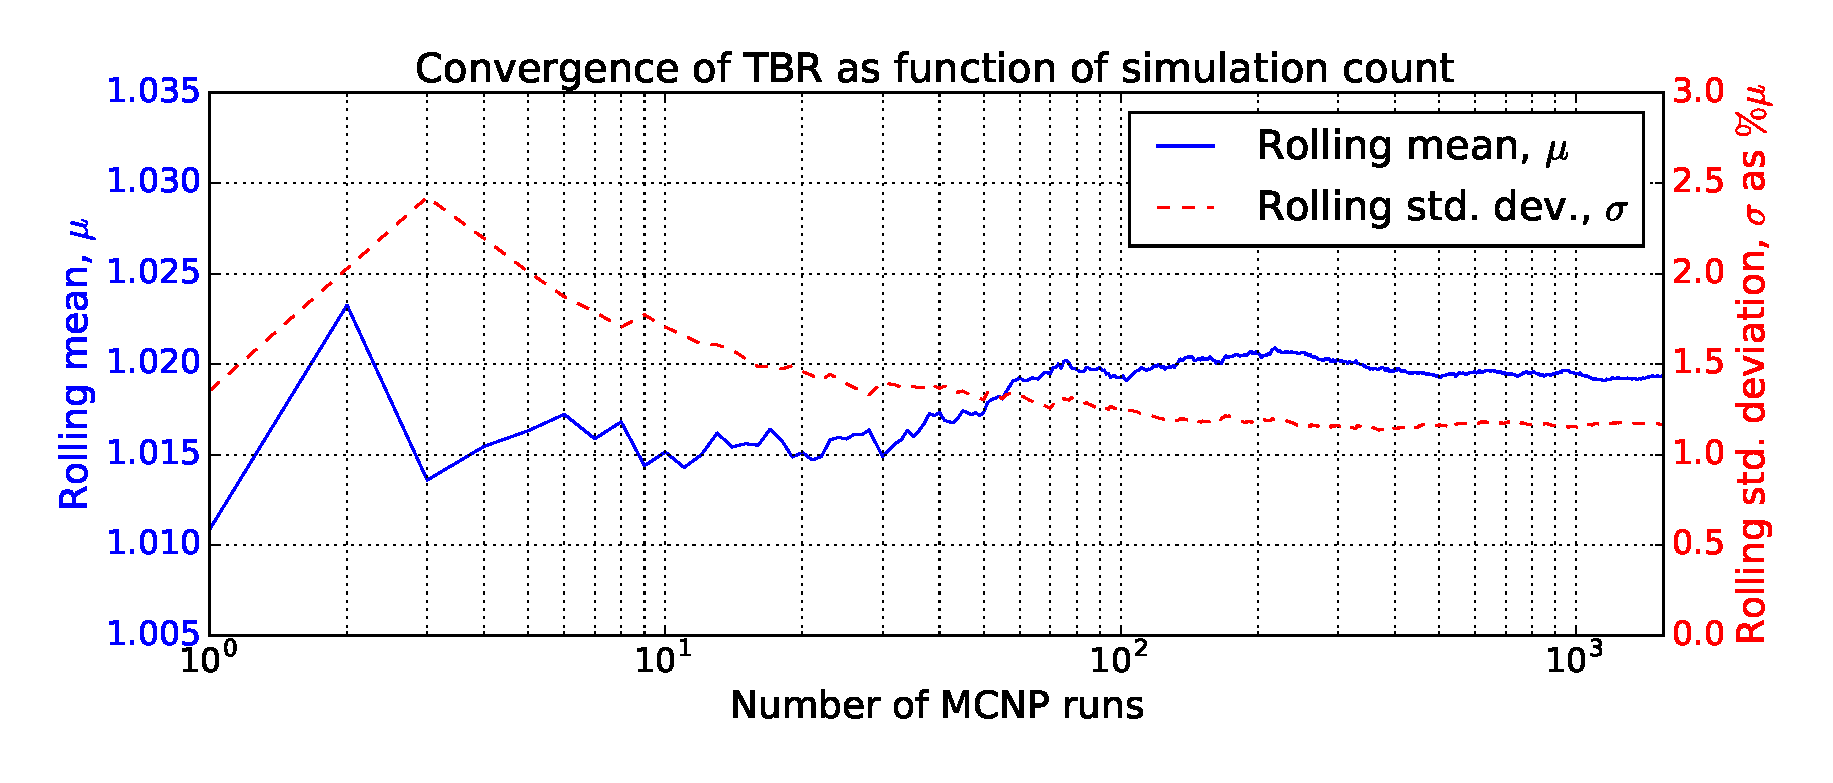
\includegraphics[width=0.8\textwidth]{hcll_convergence_1559}
	\caption[Convergence of TBR distribution as a function of simulation count.]{The simple mean and standard deviation of the TBR results is presented as a function of the number of simulations.}
	\label{fig:convergence}
\end{figure}

The TMC simulation can be seen to converge in figure~\ref{fig:convergence} at approximately 400 MCNP runs. $\mu(400) \approx 1.02$ and $\sigma(400) \approx 1.14$. The mean TBR value is 1.0193 whilst the median is 1.0200, with a one sigma standard deviation of 0.012 or 1.164\% of the mean value. 

The TBR distribution is shown as figure~\ref{fig:tbr_distribution}. Any results greater than 6$\sigma$ from the mean TBR were deemed false and discarded before analysis. This filter rejected one simulation result, where the sampled TBR value was exceptionally far from the mean value: $0.826 \approx \mu - 15\sigma$. This simulation used an erroneous \textsuperscript{207}Pb ACE file, created with unrealistic parameters. 

The shape of the distribution appears somewhat Gaussian (see equation~\ref{eq:normal}) although with an extended low-value tail. The Shapiro-Wilk test was employed to test if the TBR population have indeed been sampled from a normal distribution \cite{Shapiro1965}. Formally, a null hypothesis, $H_{0}$, that the underlying distribution is normally distributed was proposed. This hypothesis was rejected as the computed p-value for the sample population was 0.003, less than the conventional threshold for acceptance (known as $\alpha$) of 0.05\footnote{$\alpha = 0.05$ implies there is a 5\% chance the null hypothesis is incorrectly rejected and is a common value for this statistical test.}.

The distribution is fitted well with the addition of a skewness parameter, $\gamma$ to give the `skew-normal distribution' as per equation~\ref{eq:skewed_normal}. 

\begin{equation}
  \label{eq:normal}
  f(x) = \frac{1}{\omega \sqrt{2 \pi}} e^{-\frac{(x-\xi)^{2}}{2 \omega^{2}}}
\end{equation}

\begin{equation}
  \label{eq:skewed_normal}
  g(x) = f(x) \left[1 + \mathrm{erf} \left( \frac{\gamma(x - \xi)}{\omega \sqrt{2}} \right) \right]
\end{equation}

Equation~\ref{eq:skewed_normal} is the fit function plotted in figure~\ref{fig:tbr_distribution}. $\xi$ is the location parameter, $\omega$ the shape and $\gamma$ the skewness. If the data were symmetric, $\gamma = 0$. For these data, $\gamma = -1.432$, indicating the low-value TBR tail is longer than the high-value tail. 

\begin{figure}[H]
%  \figuretitle{}
  \centering
	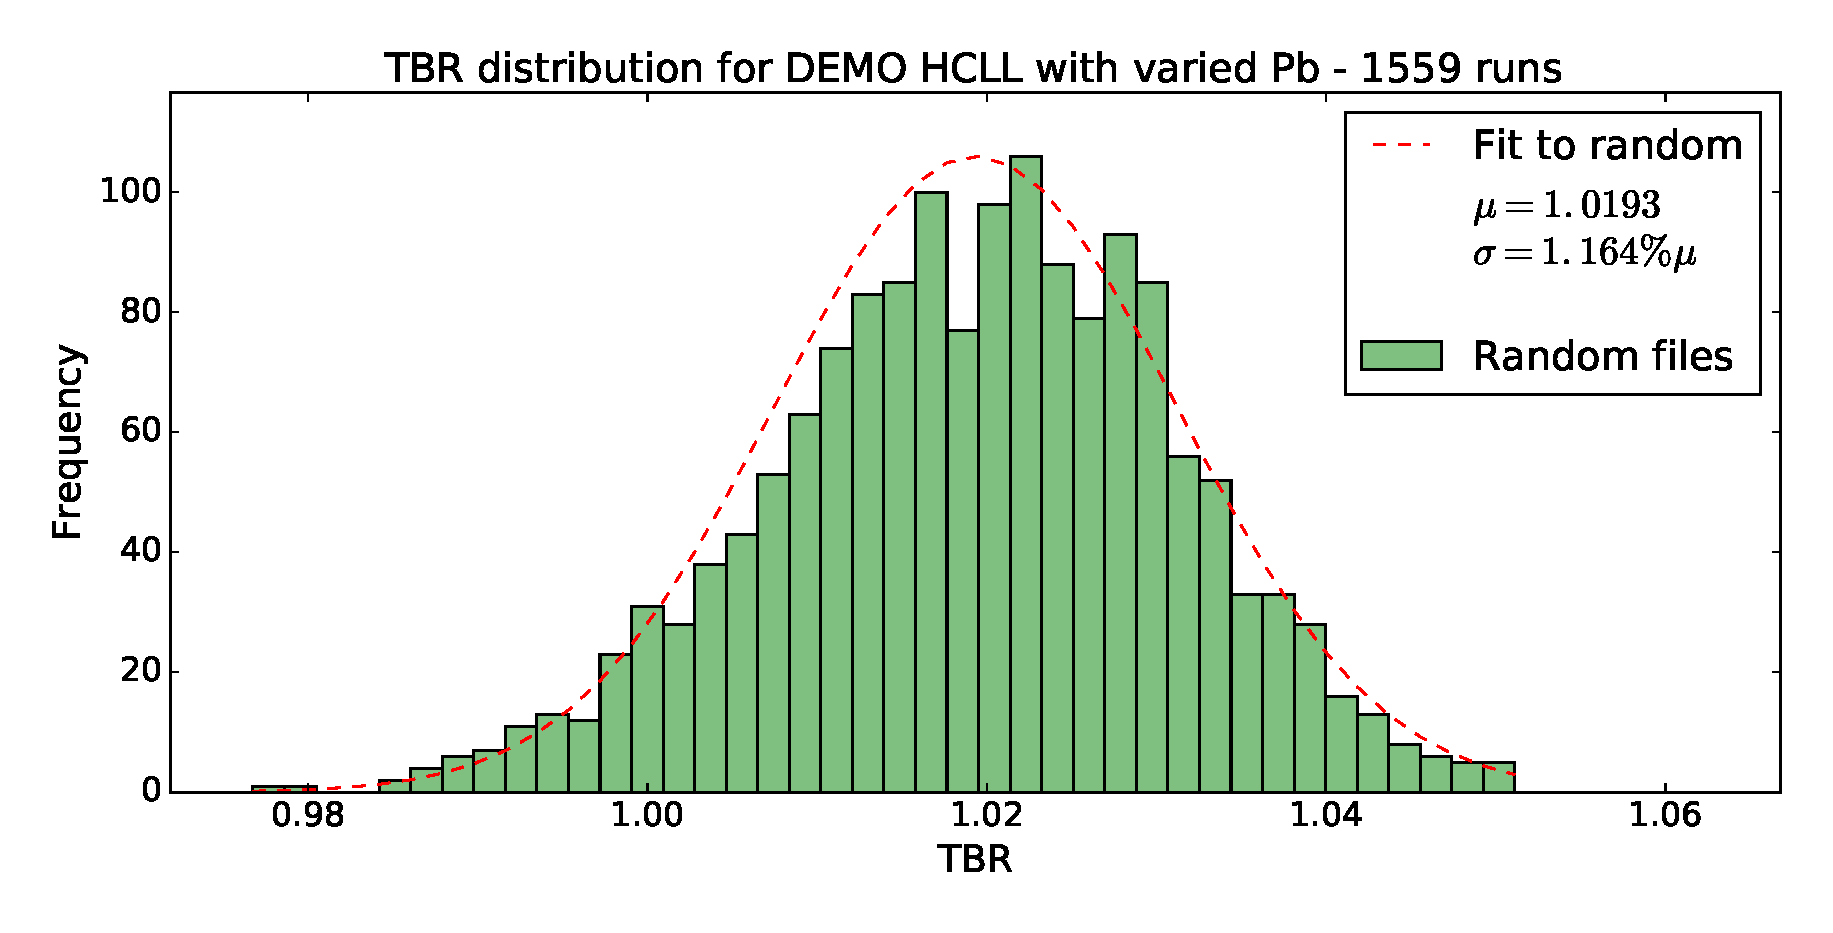
\includegraphics[width=0.8\textwidth]{hcll_hist_1559}
	\caption[DEMO HCLL TBR distribution due to lead nuclear data.]{Histogram of 1559 TBR values computed with the TMC methodology. The fit is a skew-normal distribution as described by equations~\ref{eq:normal} and \ref{eq:skewed_normal}. The standard deviation is 1.2\% of the mean value and represents the variation from TENDL2015 lead nuclear data (specifically $^{206,207,208}$Pb). Note that 5.8\% of the distribution is less than unity.}
	\label{fig:tbr_distribution}
\end{figure}

Figure~\ref{fig:tbr_n2n} shows the correlation between the n,2n cross-sections used in a given simulation and the TBR attained in that simulation. The nuclide-wise cross-sections were obtained with the Inter utility for a reaction energy of 14 MeV. As the cross-sections for each of the three lead isotopes were varied in every simulation, so the cross-sections plotted here are the elemental average values, that is, weighted by the natural abundance of each Pb isotope. A linear least squares fit has been applied to the data shown in figure~\ref{fig:tbr_n2n} and the resulting relationship plotted in blue. As the cross-section for neutron multiplying reactions of the form $^{A}$Pb(n,2n)$^{A-1}$Pb increases, so does the neutron flux available for the subsequent generation of tritium in the breeding blanket. As these reactions are endothermic, with an energy threshold relatively close to that of the D-T neutron creation energy, front loading a breeding blanket with neutron multiplying material is beneficial to TBR.

\begin{figure}[H]
%  \figuretitle{}
  \centering
	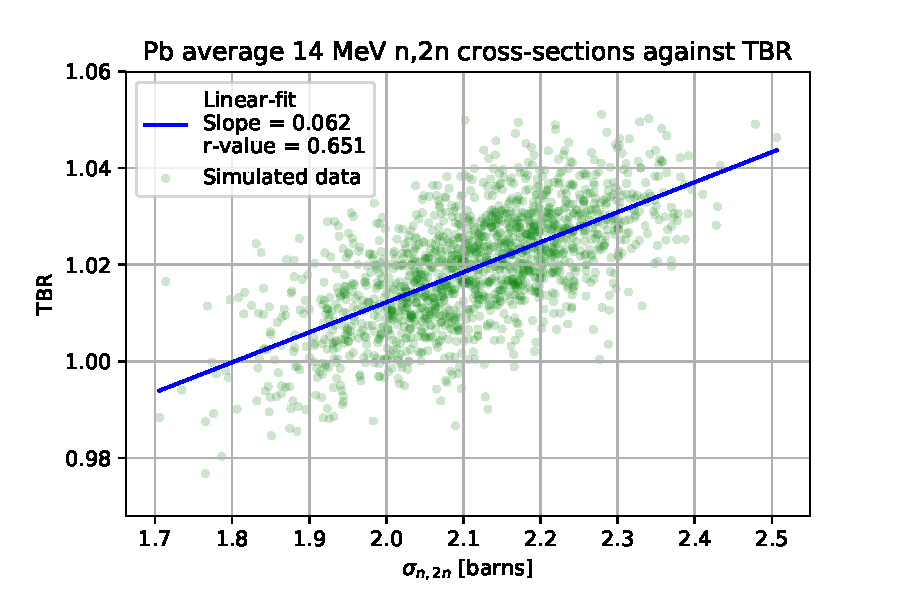
\includegraphics[width=0.7\textwidth]{TBR_n,2n}
	\caption[Correlation between $^{208}$Pb(n,2n)$^{207}$Pb cross-sections and TBR.]{Shown here are the $^{208}$Pb(n,2n)$^{207}$Pb cross-sections at 14 MeV, from the files used as input ND for the TMC simulation. They are plotted against the resulting TBR value from each simulation. There is a reasonably strong positive correlation, with increasing n,2n cross-sections resulting in an increased TBR.}
	\label{fig:tbr_n2n}
\end{figure}

The relationship between n,2n cross-section and TBR shown in figure~\ref{fig:tbr_n2n} is relatively strong, with a linear fit achieving an $r^{2}=0.42$, explaining 42\% of the total variance in TBR. Elastic scattering (shown in figure~\ref{fig:tbr_elastic}) is more weakly correlated, with a very low $r^{2}=0.02$. Figures~\ref{fig:tbr_n2n} and \ref{fig:tbr_elastic} plot relationships between the cross-section values and the simulated TBR result, but these cross-sections are only intermediate data in the TMC process. However it is possible to go one step further back and analyse for correlations between fundamental nuclear parameters and the observable of interest, TBR. 

\begin{figure}[H]
%  \figuretitle{}
  \centering
	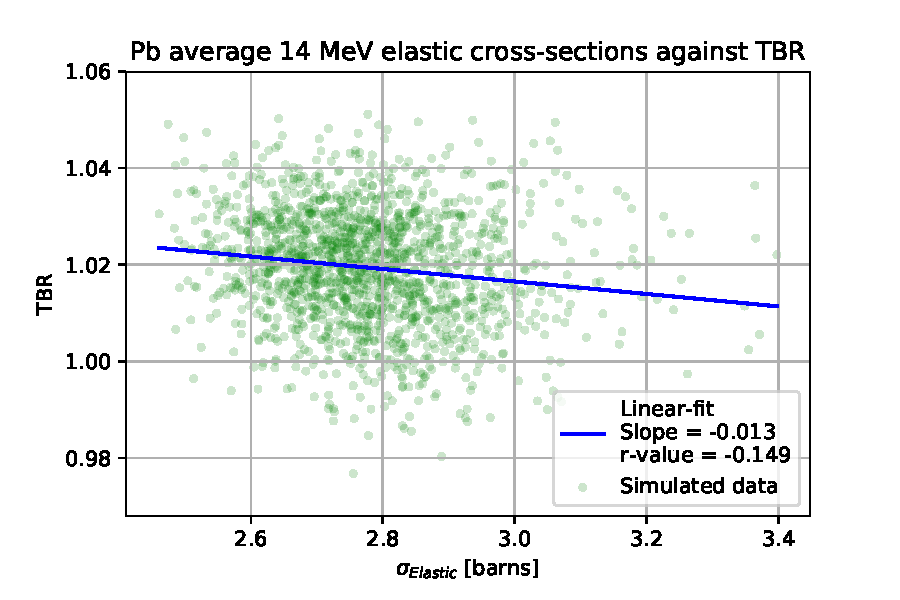
\includegraphics[width=0.7\textwidth]{TBR_Elastic}
	\caption[Correlation between $^{208}$Pb(n,el)$^{208}$Pb cross-sections and TBR.]{Shown here are the $^{208}$Pb(n,el)$^{208}$Pb cross-sections at 14 MeV, from the files used as input ND for the TMC simulation. They are plotted against the resulting TBR value from each simulation. There is a weak correlation, with a minor downward trend in TBR for increasing elastic cross-section.}
	\label{fig:tbr_elastic}
\end{figure}

The optical model is a nuclear model which aims to describe the interaction between an incident nucleon and a target nucleus. Rather than trying to solve particle behaviour \textit{ab initio}, this approach uses a complex potential energy function or simply `potential', $\mathcal{U}$ to represent nucleon-nucleus interactions. This potential energy function is a kind of description of the strong nuclear force, as a nucleon far from the nucleus, outside of the range of this force will experience no interaction. Closer, where the separation distance $r$ becomes similar to the nuclear radius $R$ and the particle may fall into the nucleus' potential well. Solving the Schr\"odinger equation with a given potential generates predictions for basic observables such as elastic scattering angular distributions and possibly the reaction and total cross-sections \cite{Hodgson1971}. 

The optical model's name is due to an analogous case where a light wave is part refracted and part absorbed in a material of complex refractive index. The imaginary part of the complex refractive index is responsible for the absorption of light. In the nuclear case, the imaginary part of the nuclear potential represents all the non-elastic behaviour. An optical model potential (OMP) contains parameters and can be fit to experimental data. In this case the optical model is known as phenomenological. In part because of the wealth of experimental nuclear physics data now available, there has been a great advance in the capabilities and generality of the optical model since its first iteration by \citeauthor{Fernbach1949} in 1949. Fits to experimental data can be global, determining parameter values which best fit a wide range of energies and nuclei, or local, where a fit is determined for a sole nucleus. These local fits produce more accurate results but clearly have worse predictive power for other situations outside of their fit parameters.

The TENDL team used the T6 package to generate the TENDL2015 data employed for this work. The nuclear reaction program within this suite, TALYS, employs the optical model specified by \citeauthor{Koning2003}. The potential $\mathcal{U}$ has contributions from the terms in equation~\ref{eq:talys_omp}. 

\begin{equation}
  \mathcal{U}(r,E) = - \mathcal{V}_{V}(r,E) - i\mathcal{W}_{V}(r,E) - i\mathcal{W}_{D}(r,E) + \mathcal{V}_{SO}(r,E) + i\mathcal{W}_{SO}(r,E)
  \label{eq:talys_omp}
\end{equation}

Where $\mathcal{V}_{V,SO}$ and $\mathcal{W}_{V,D,SO}$ are the real and imaginary components of the volume (V), surface (D), and spin-orbit (SO) potentials respectively. Each of these terms is separated into an energy dependent well-depth and an energy-independent radius dependent component\footnote{See §4.1.1 in \cite{TALYS2017} for more detail}. The general form of the radius dependent part for all the potentials is a Woods-Saxon shape \cite{Woods1954} as shown in equation~\ref{eq:woods-saxon}.

\begin{equation}
  \label{eq:woods-saxon}
  f(r,R,a) = \left(1 + e^{\frac{r-R}{a}}\right)^{-1}
\end{equation}

Where $r$ is the separation, $a$ a `diffuseness' parameter and $R$ the nuclear radius. $r_{V}$ is equivalent to the nuclear radius parameter $R$ in equation~\ref{eq:woods-saxon} for the $\mathcal{V}_{V}$ and $\mathcal{W}_{V}$ terms of the OMP shown as equation~\ref{eq:talys_omp}. The distribution of $r_{V}$ values that were sampled in the creation of $^{207}$Pb data for this study is shown as figure~\ref{fig:pb207_rvadjust_hist}. It is uni-modal, non-normally distributed and positively skewed. 

\begin{figure}[H]
%  \figuretitle{}
  \centering
	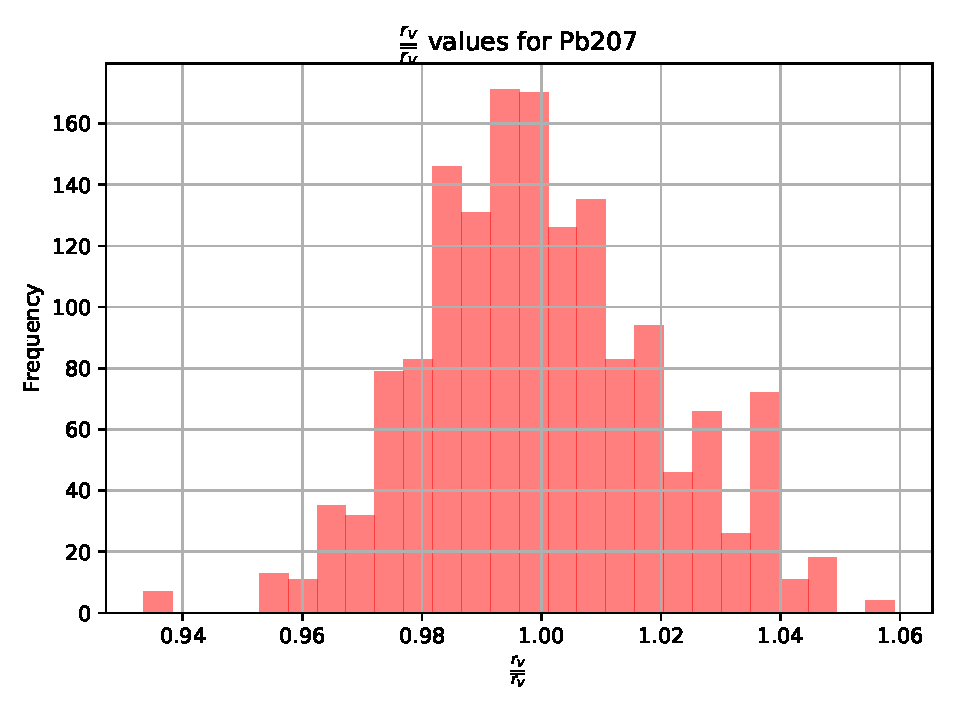
\includegraphics[width=0.8\textwidth]{rvadjust_param_Pb207_histogram}
	\caption[$r_{V}$ nuclear parameter distribution for $^{207}$Pb.]{This figure shows the distribution of nuclear radius, or $r_{V}$ values sampled in the creation of $^{207}$Pb cross-section data for this TMC work. $r_{V}$ is a geometry parameter in optical model potentials. The distribution is slightly positively skewed. The data here have been normalised by their mean to centre the distribution on unity and allow for easier comparison between parameters of different scale.}
	\label{fig:pb207_rvadjust_hist}
\end{figure}

Shown as figure~\ref{fig:pb207_rvadjust} is the relationship between $r_{V}$ as shown in figure~\ref{fig:pb207_rvadjust_hist}, as applied to the generation of \textsuperscript{207}Pb data, to the resulting TBR values. The data in figure~\ref{fig:pb207_rvadjust} have a weak relationship. A linear least squares fit is shown, with a positive slope of $m=0.06$. The $r^{2}$ value is very low at 0.01. This implies, as can be seen visually, that a great deal of variance in the data is left unexplained by the fit. However, this study has varied several nuclear parameters and nuclides simultaneously--were fewer inputs varied the relationship shown in figure~\ref{fig:pb207_rvadjust} might be clearer. 

Figure~\ref{fig:pb207_d1adjust} shows TBR data plotted against the values of nuclear parameter $d_{1}$ used in the simulation input data. This parameter has the highest correlation coefficient, $r^{2}$ of any parameter for $^{207}$Pb.

\begin{figure}[H]
%  \figuretitle{}
  \centering
	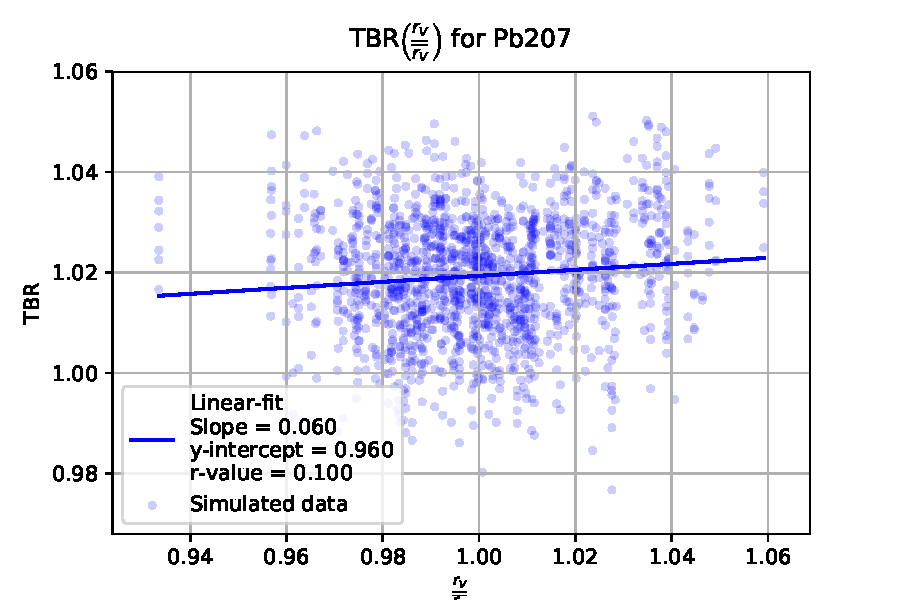
\includegraphics[width=0.7\textwidth]{Pb207_rvadjust}
	\caption[TBR as a function of $r_{V}$ for $^{207}$Pb.]{Scatter plot of the $r_{V}$ nuclear radius parameter against simulated TBR. The $r_{V}$ values have been normalised to the mean of their distribution, centring the distribution on unity. The data has been fit with a linear relationship, with the fit data shown in the plot. A minor positive correlation is registered.}
	\label{fig:pb207_rvadjust}
\end{figure}

\begin{figure}[H]
%  \figuretitle{}
  \centering
	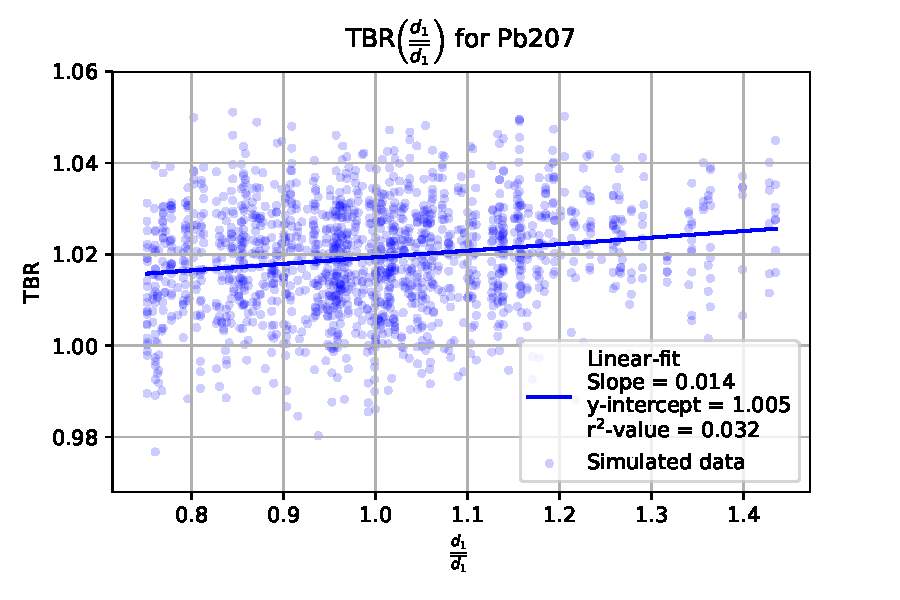
\includegraphics[width=0.7\textwidth]{Pb207_d1adjust}
	\caption[TBR as a function of $d_{1}$ for $^{207}$Pb.]{Scatter plot of the $d_{1}$ parameter against simulated TBR. The $d_{1}$ values have been normalised to the mean of their distribution, centring the distribution on unity. The data has been fit with a linear relationship, with the fit data shown in the plot. A positive correlation is registered.}
	\label{fig:pb207_d1adjust}
\end{figure}

Performing a least-squares fit on all the varied nuclear parameters against the simulated TBR results, we can estimate which parameters TBR is most correlated with. For \textsuperscript{207}Pb the parameter correlation bar chart is shown as figure~\ref{fig:pb207_param_correl}, with the ordinate displaying the $r^{2}$ of the linear regression. Prior to fitting, the parameters were normalised to their mean value. It can be seen that the sampled variation in the $d_{1,3}, w_{2}, r_{V}$ and $a_{v}$ parameters for \textsuperscript{207}Pb result in the most change in simulated TBRs. The parameter most strongly correlated with TBR for $^{206}$Pb and $^{208}$Pb is $d_{1}$, a multiplicative parameter in the energy dependent component of $\mathcal{W}_{D}$, the imaginary surface potential. Better constraining these parameters might act to reduce uncertainty in future lead based blanket analyses. This could be achieved with more experimental data or advances in model theory.

\begin{figure}[H]
%  \figuretitle{}
  \centering
	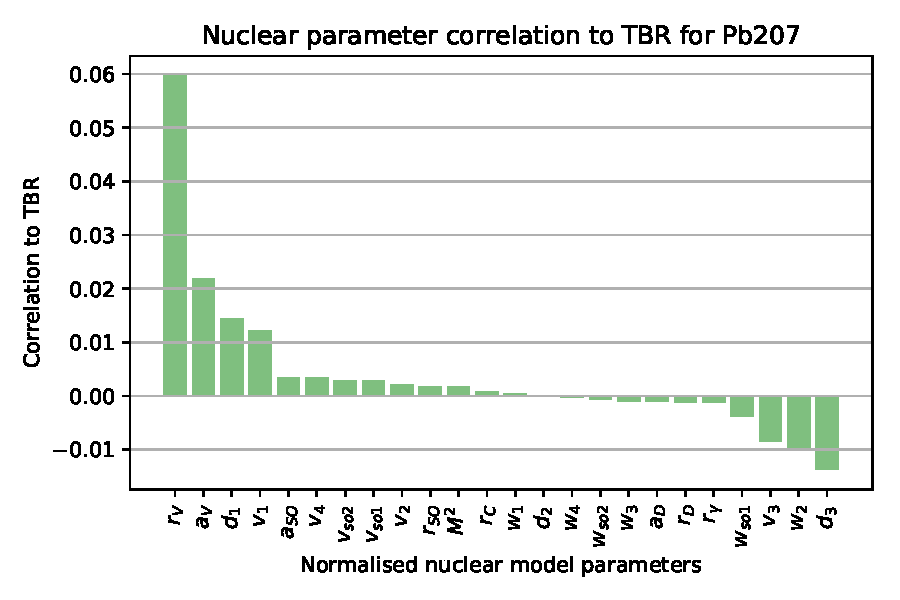
\includegraphics[width=0.8\textwidth]{Pb207_param_correl}
	\caption[Strength of correlation between $^{207}$Pb nuclear parameters and TBR.]{This bar chart shows the relationship between various nuclear parameters and TBR simulation data. The abscissa shows a variety of model parameters, the vast majority from optical model potentials. The ordinate values for each parameter are measures of the correlation between sampled parameter data and the TBR. The correlation measure is the r-squared value of a linear fit to each dataset. The parameter data was normalised to its mean before fitting. The majority of parameters studied have little correlation with TBR, leaving a few optical model parameters such as $r_{V}$ and $d_{1}$.}
	\label{fig:pb207_param_correl}
\end{figure}

% \begin{figure}[H]
% %  \figuretitle{}
%   \centering
%   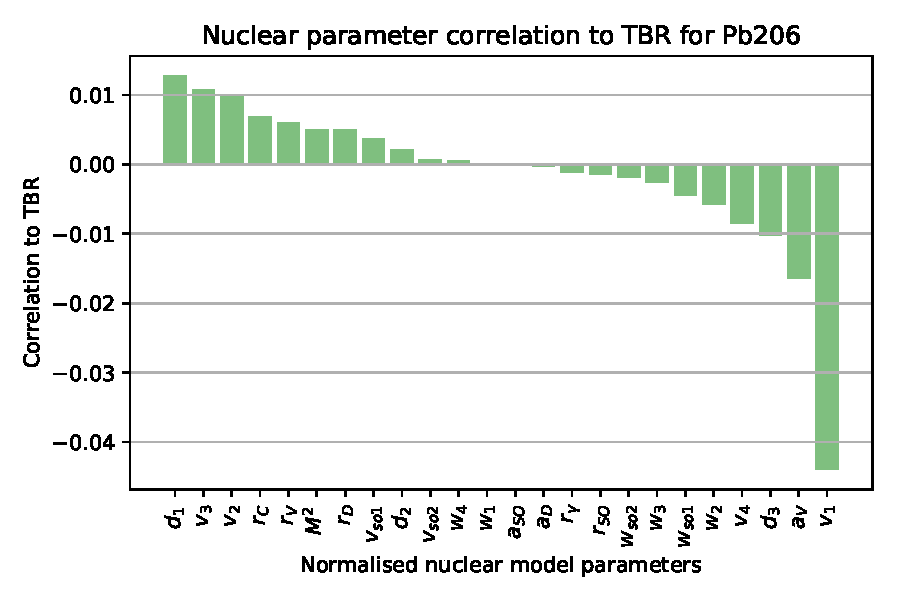
\includegraphics[width=0.8\textwidth]{Pb206_param_correl}
%   \caption{}
%   \label{fig:pb206_param_correl}
% \end{figure}
%
% \begin{figure}[H]
% %  \figuretitle{}
%   \centering
%   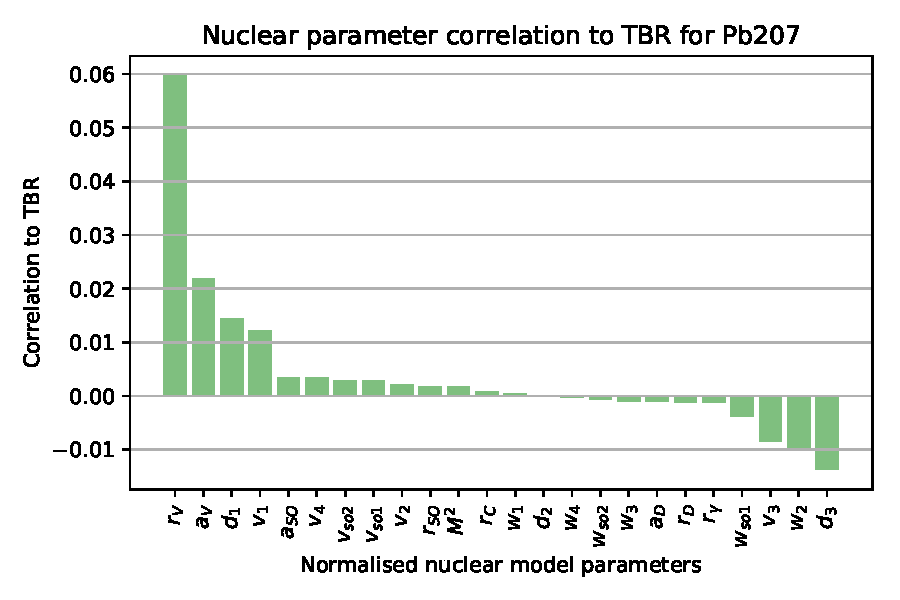
\includegraphics[width=0.8\textwidth]{Pb207_param_correl}
%   \caption{}
%   \label{fig:pb207_param_correl}
% \end{figure}

%%%%% WARNING ---->
% Even energy dependent adjustment of the geometry is possible as a last resort to fit data, using the rvadjustF, etc. keywords.
% Have we found a strong correlation between a fudge parameter and the TBR? Oh dear

\section{Conclusion}
TBR uncertainty has been computed with the TMC technique, investigating the contribution of uncertain nuclear data from the three major lead isotopes. The standard deviation is 1.2\% of the mean TBR. However, note that 5.8\% of the distribution is less than unity. While the average value may appear to be feasible, it should be stressed that there is a non-negligible probability of a value below a required limit. The TBR values are relatively low as this particular model has not been optimised for TBR and any practical design should have a TBR $\approx 1.1$ \cite{Fischer2015}, but in future design studies engineers should be aware of the probability of non-compliant operational parameters. 

The TENDL-2015 nuclear data investigated in section \ref{subsec:data}, which is not necessarily Gaussian in shape, has yielded a TBR distribution with a small but finite negative skewness, an extended low-value tail. Decreasing the uncertainty in the aforementioned important optical model parameters, such as $d_{1}$ for Pb, would potentially act to reduce the uncertainty in future TBR analyses.

Uncertainty propagation in Monte-Carlo type radiation transport problems has often previously been computed using linear perturbation theory approaches. Unfortunately these are only applicable for small changes in the input data. They are also unable to reproduce probability distributions of the integral quantity of interest \cite{Rising2012}. Whilst figure \ref{fig:tbr_distribution} shows a TBR distribution that is only slightly skewed, that is not to say other fusion quantities will not be. Koning \& Rochman have demonstrated that fast and accelerator driven fission systems can have significantly skewed $k_{\mathrm{eff}}$ values, well described by an Extreme Value Fit (EVD) \cite{Koning2008}.

Future work on TBR in HCLL could include the effect of other nuclides and elements which TBR is sensitive to including iron and oxygen as well as a completely correlated uncertainty propagation method employing lithium if data for light nuclides becomes available.

More generally, when solving for integral quantities in nuclear fusion systems, thought should be given to fully-correlated uncertainty propagation and the form of the resulting probability distributions. In particular, whether a non-normal distribution with increased likelihood of extreme behaviour would have engineering design or safety implications for TBR, nuclear heating, fast flux, gas production or damage terms. Moreover, in all analyses for design applications the non-negligible probability of operational parameters in unacceptable regimes should be borne in mind.


%!TEX root = ../thesis.tex
%*******************************************************************************
%****************************** Second Chapter *********************************
%*******************************************************************************

\chapter{Quantifying received dose errors introduced by spatial homogenisation of reinforced concrete shielding}

\ifpdf
    \graphicspath{{Chapter2/Figs/Raster/}{Chapter2/Figs/PDF/}{Chapter2/Figs/}}
\else
    \graphicspath{{Chapter2/Figs/Vector/}{Chapter2/Figs/}}
\fi


\section{Outline}

%INTRODUCTION
\section{Introduction}
An investigation into the process of spatial homogenisation of radiation transport geometry has been performed for reinforced concrete shielding. Using parameters relevant for the ITER fusion experiment, shielding and activation simulations have quantified the effect of homogenisation. The dose received by a person beyond the shield during plasma operation is underestimated by homogenisation. For walls over a meter in thickness it can be by 20\%. The shut down dose to a worker on the tokamak side of an activated wall \textit{due to the wall} is overestimated by homogenisation, by a factor of up to 60.

In nuclear engineering, quantifying the absorbed dose to radiation sensitive components, or the equivalent dose to personnel usually requires crafting a computer model of the problem, making a series of assumptions and simplifications in the process. For reinforced concrete radiation shields, this often entails either homogenising the reinforcing bar (abrev. rebar) with the concrete, or even neglecting the presence of rebar entirely. However, steel has a high density $\sim7.8g\cdot cm^{-3}$ and a markedly different elemental composition to low density $\sim2.2g\cdot cm^{-3}$ concrete. Steel is an alloy of many different elements but principally high-Z Fe. Whereas concrete largely consists of low-Z elements, O, Si \& H (in descending atomic density order).\par
The process of homogenisation introduces systematic error into the reported solution of any radiation transport problem by moving steel and adjusting the density.

The discrepancy in results between heterogeneous and homogeneous modelling approaches is investigated in this work. Querying the strength of correlation of the discrepancy with a given parameter requires producing radiation transport geometry in pairs, as shown in figure \ref{fig:wall_diagram}. 

\subsection{Literature review}

\subsection{ITER}

% column span figure
\begin{figure}[H]
  \figuretitle{Homogenising reinforced concrete}
	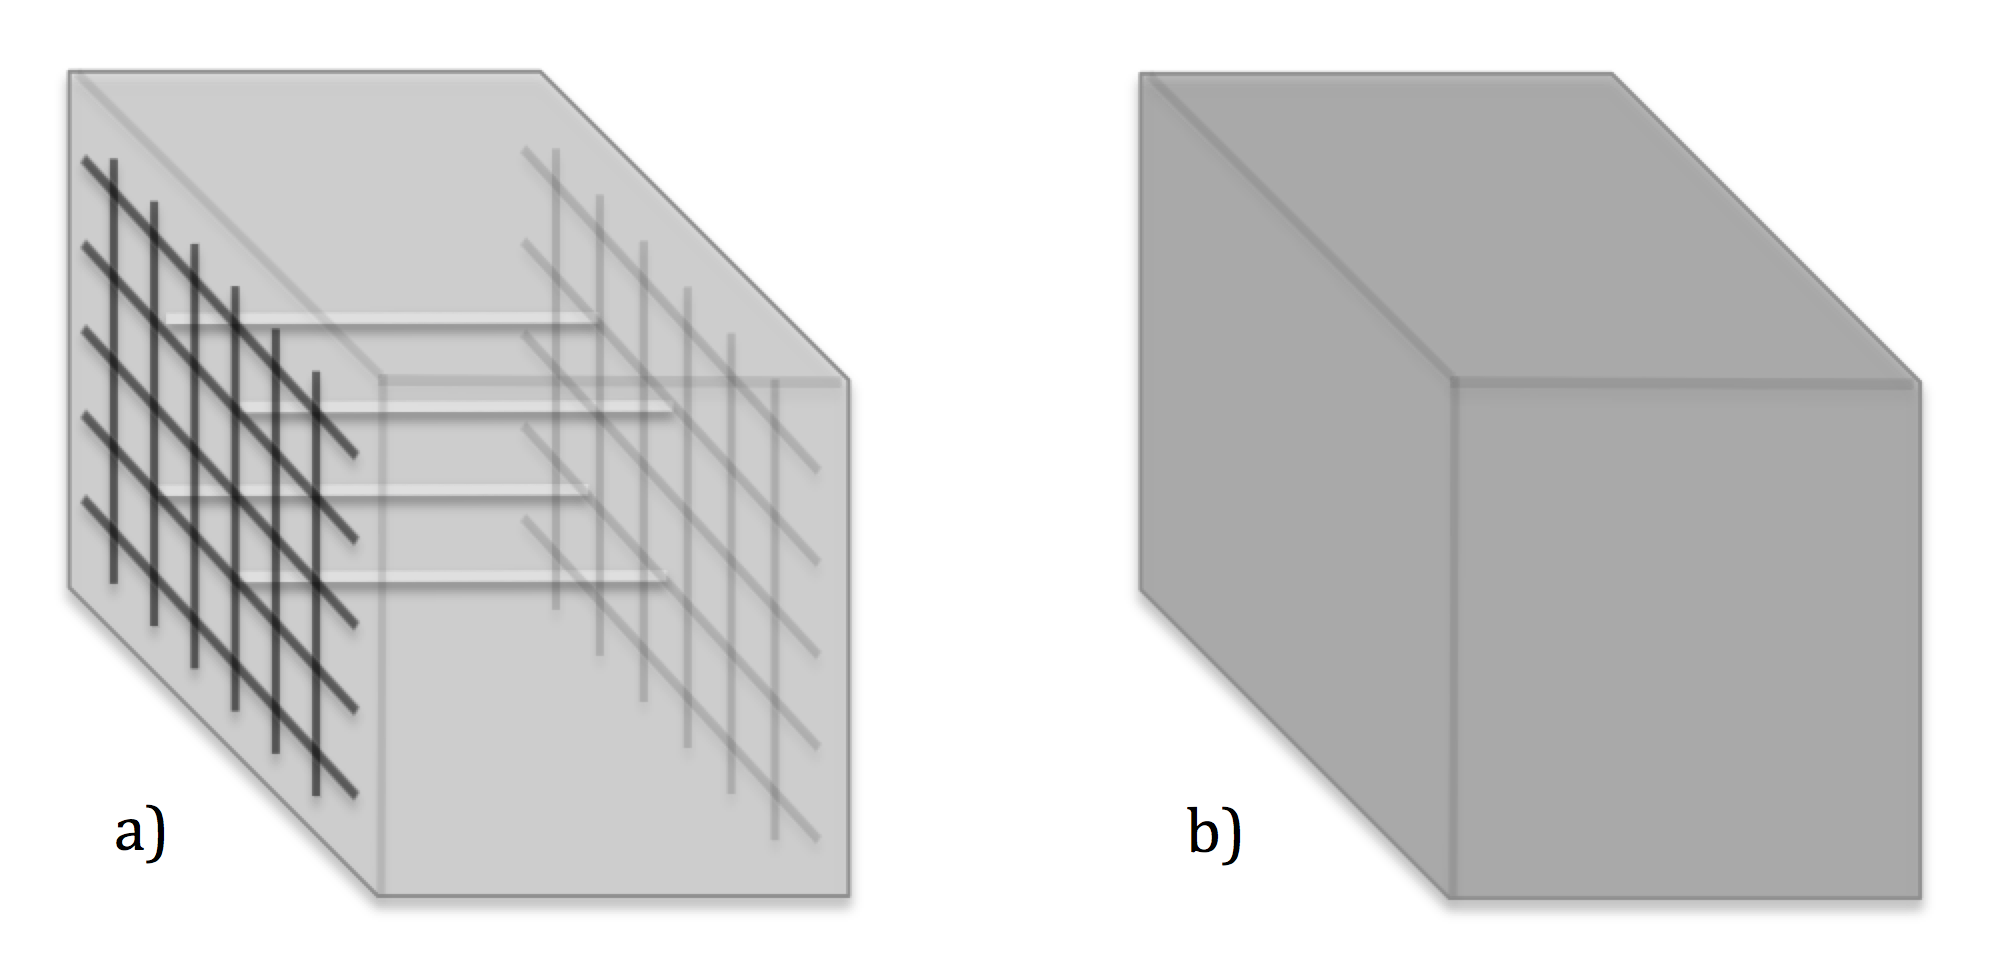
\includegraphics[width=\textwidth]{wall_diagram}
	\caption{The two modelling approaches considered in this investigation. a) Heterogeneous, where the steel reinforcing bar and stirrups are explicitly modelled. b) Homogeneous, where the mass of rebar is 'smeared' through the concrete. The new homogenised material has a greater density than plain concrete, conserving mass.}
	\label{fig:wall_diagram}
\end{figure}

The heterogeneous wall is constructed of a large concrete block, with two meshes of rebar, one buried below each face. The distance from wall exterior to rebar is known as the cover depth. Connecting the two meshes are a small number ($4m^{-2}$) of narrow gauge stirrup bars.

Material compositions, wall widths, rebar arrangements and steel fractions have been determined from ITER drawings and specifications for concrete walls in the tokamak building. The results should give a good idea of the implications of the homogeneous modelling approximation at ITER. The work was also conducted with a moderated ITER DT fusion neutron source spectrum. As such, this investigation should not only be instructive concerning ITER shielding, but also other DT fusion facilities.

%METHOD
\section{Method}

The principal modelling simplification under investigation is that of spatial homogenisation. As such, for each set of independent and dependent variables, at least two simulations will be performed. One will have a high-fidelity model of the real-world problem geometry with rebar and stirrups faithfully reproduced. The other will smear the rebar across the concrete, homogenising the two materials into one with a density equal to the mass weighted sum of the concrete and steel constituents. \par
The implications of homogenisation prove to be different for on-load and shut-down (activated) dose rates. It is helpful to consider them seperately.

\subsection{Prompt neutron \& gamma radiation}

Determining the dose to personnel beyond a wall requires knowledge of the radiation fluxes there. The on-load gamma flux $\phi_{\gamma}(x,y,z,E,t)$ and neutron flux, $\phi_{n}(x,y,z,E)$, can be computed with Monte Carlo techniques, spawning neutrons from a prerecorded source distribution, $P(x,y,z,E,\Omega)$ at a particular point with a given energy and angle. These particles may propagate through the wall, scattering, being absorbed, exciting nuclei (which later relax through radiative emission) and perhaps leaking out of the back of the shield wall. Tallying this leakage flux of neutrons and photons is the main task of calculating a dose due to radiation.\par
Radiation transport was conducted with MCNP6v1.0. The nuclear data employed was the continuous energy Joint Evaluated Fission and Fusion file 3.2 (JEFF3.2) for neutron transport and MCPLIB84 for photon transport. Input decks for MCNP were produced with a bespoke Python program written by the author, this automated approach allowed for easy parametric study. \par
The MCNP relative error, $R = \frac{\sigma_{s}}{\mu_{s}}$ which is the ratio of sample standard deviation to sample mean was kept to below 0.1 for all energy bins and mesh voxels.

% column span figure
\begin{figure}[H]
  \figuretitle{Neutron source spectrum}
	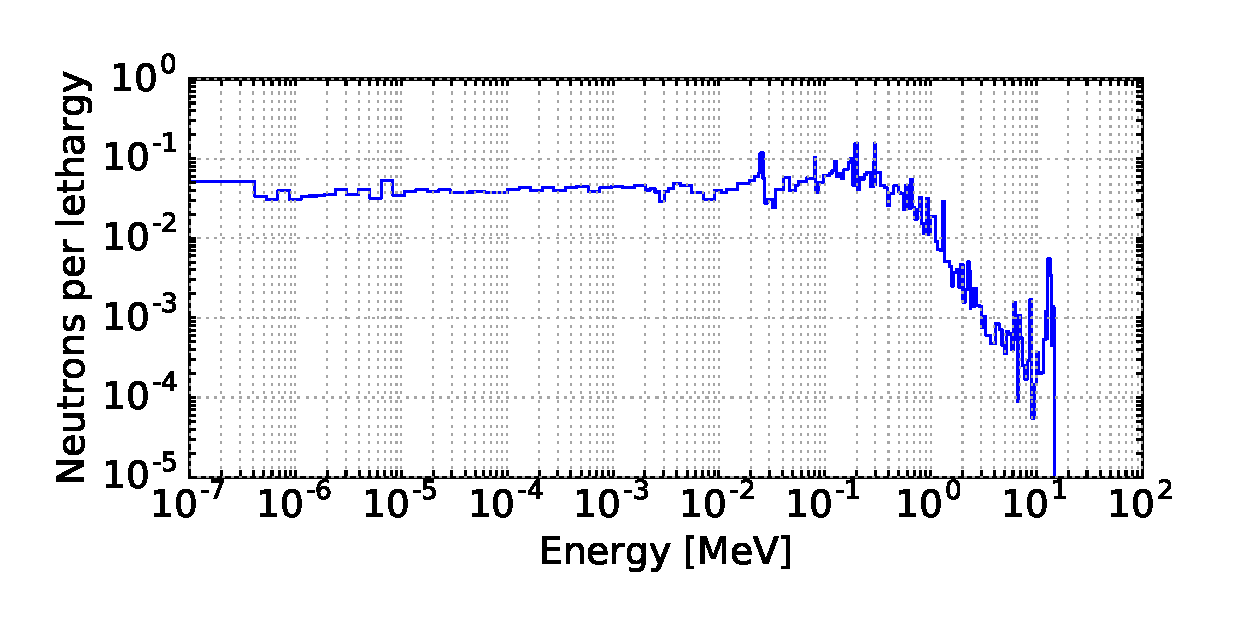
\includegraphics[width=\textwidth]{src_spectra}
	\caption{Neutron spectra for incident radiation. This spectra was recorded in 175 energy groups from the back of the ITER Neutral Beam assembly, immediately inside the bioshield concrete wall.}
	\label{fig:src_spectra}
\end{figure}

The source spectrum plotted as figure \ref{fig:src_spectra} has the recognisable DT peak, but has been significantly thermalised. The apparent absence of a Maxwellian shape around the facility temperature is because of the coarse energy binning used for this tally.

% column span figure
\begin{figure}[H]
  \figuretitle{ICRP74 flux to dose factors}
	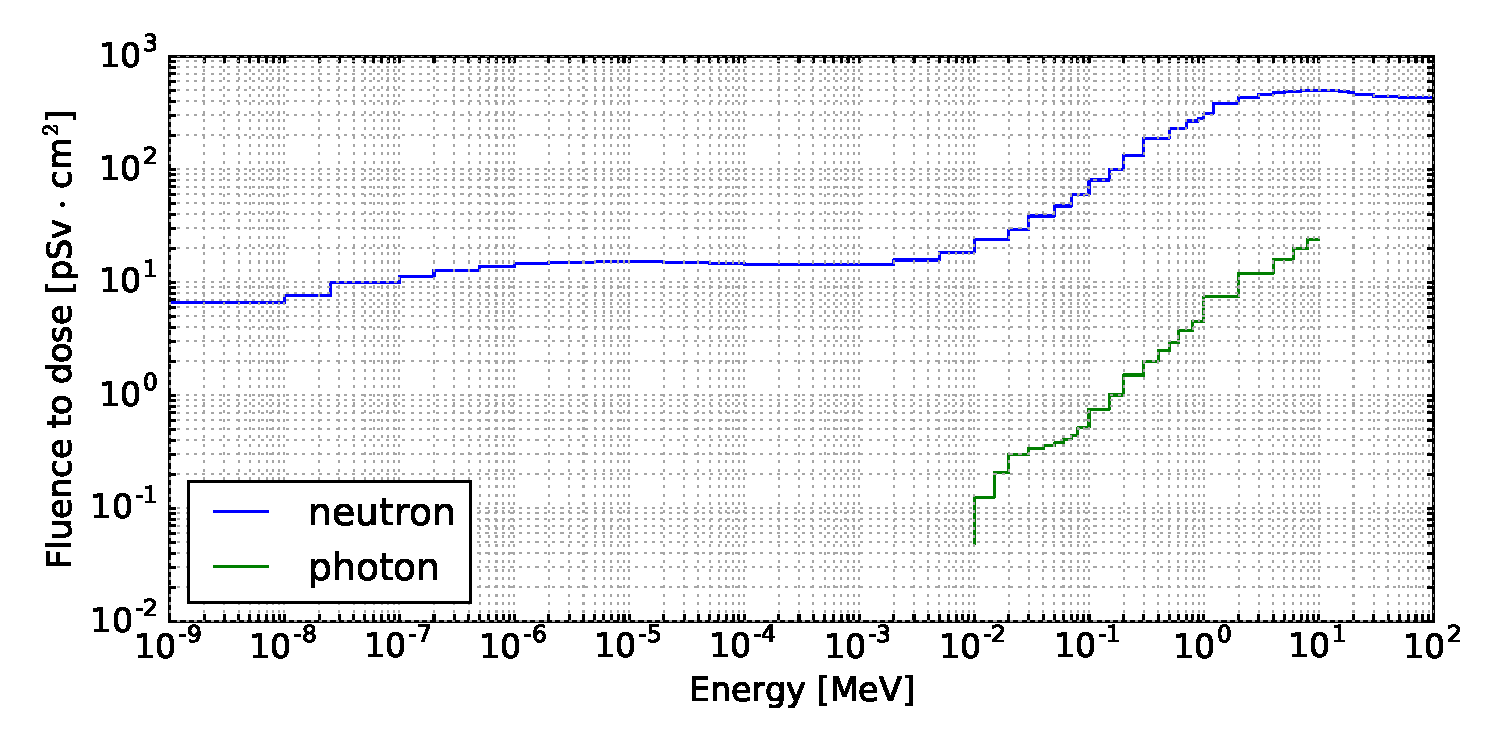
\includegraphics[width=\textwidth]{icrp74}
	\caption{The flux to dose conversion factors for neutron and photon exposure.}
	\label{fig:icrp74}
\end{figure}

The effective dose to humans is a function of the energy and type of radiation. It takes into account the varying susceptibilities of different tissues in the human body. For radiation protection, this is the typical figure quoted when specifying a dose rate. Translation from fluence or flux is by a table similar to that plotted as figure \ref{fig:icrp74}.

%\begin{equation}
%\lambda_{D(e)}=\sqrt{ \frac{ \varepsilon_0 k_B T_{(e)}}{e^2 n_\infty}}
%\end{equation}

\subsection{Delayed gamma radiation}

The calculation of $\phi_{\gamma}(x,y,z,E,t)$ where $t$ is some time after cessation of plasma operation comprises three main steps:
\begin{enumerate}
  \item 1) Neutron transport---as previously, compute the neutron flux during plasma operation, $\phi_{n}(x,y,z,E)$, recording the neutron flux binned by energy over a spatial mesh. 
  \item 2) Activation---determine the appropriate irradiation scenario, then activate and transmutate the materials present in the problem geometry. 
  \item 3) Photon transport---using the distributed decay gamma source produced by step 2), conduct a radiation transport run to determine the photon flux, $\phi_{\gamma}(x,y,z,E,t)$, converting to effective dose as required.
\end{enumerate}

As for before, radiation transport was conducted with MCNP6 v1.0. Activation was conducted with the FISPACT-II code and EAF2010 nuclear data. \par
The irradiation scenario employed for the activation step was ITER's SA-2, which gives a good representation of the ITER experimental programme total fluence and of the final, end-of-life pulses.

%\end{multicols}

%%%%%%%%%%%%%%%%%%%%%%%%%%
% RESULTS AND DISCUSSION %
%%%%%%%%%%%%%%%%%%%%%%%%%%
\section{Results \& discussion}
%\begin{multicols}{2}

\subsection{Transmission of prompt radiation}
\label{subsec:prompt}
The leakage neutron spectra for a thick (2.1m) concrete wall is shown below as figure \ref{fig:trans_neutron_spec}. The flux has been severely reduced by its interaction with the wall, decreasing from the source by an order of magnitude each 20cm traversed.\par
The reduced thermal flux in the homogeneous case is in part because steel is now available for neutron interactions throughout the depth of the wall. Steel has a greater combined capture cross-section than concrete (radiative capture shown in figure \ref{fig:n_rad_capture}), this acts as a neutron sink. 

% column span figure
\begin{figure}[H]
  \figuretitle{Transmitted neutron spectra}
	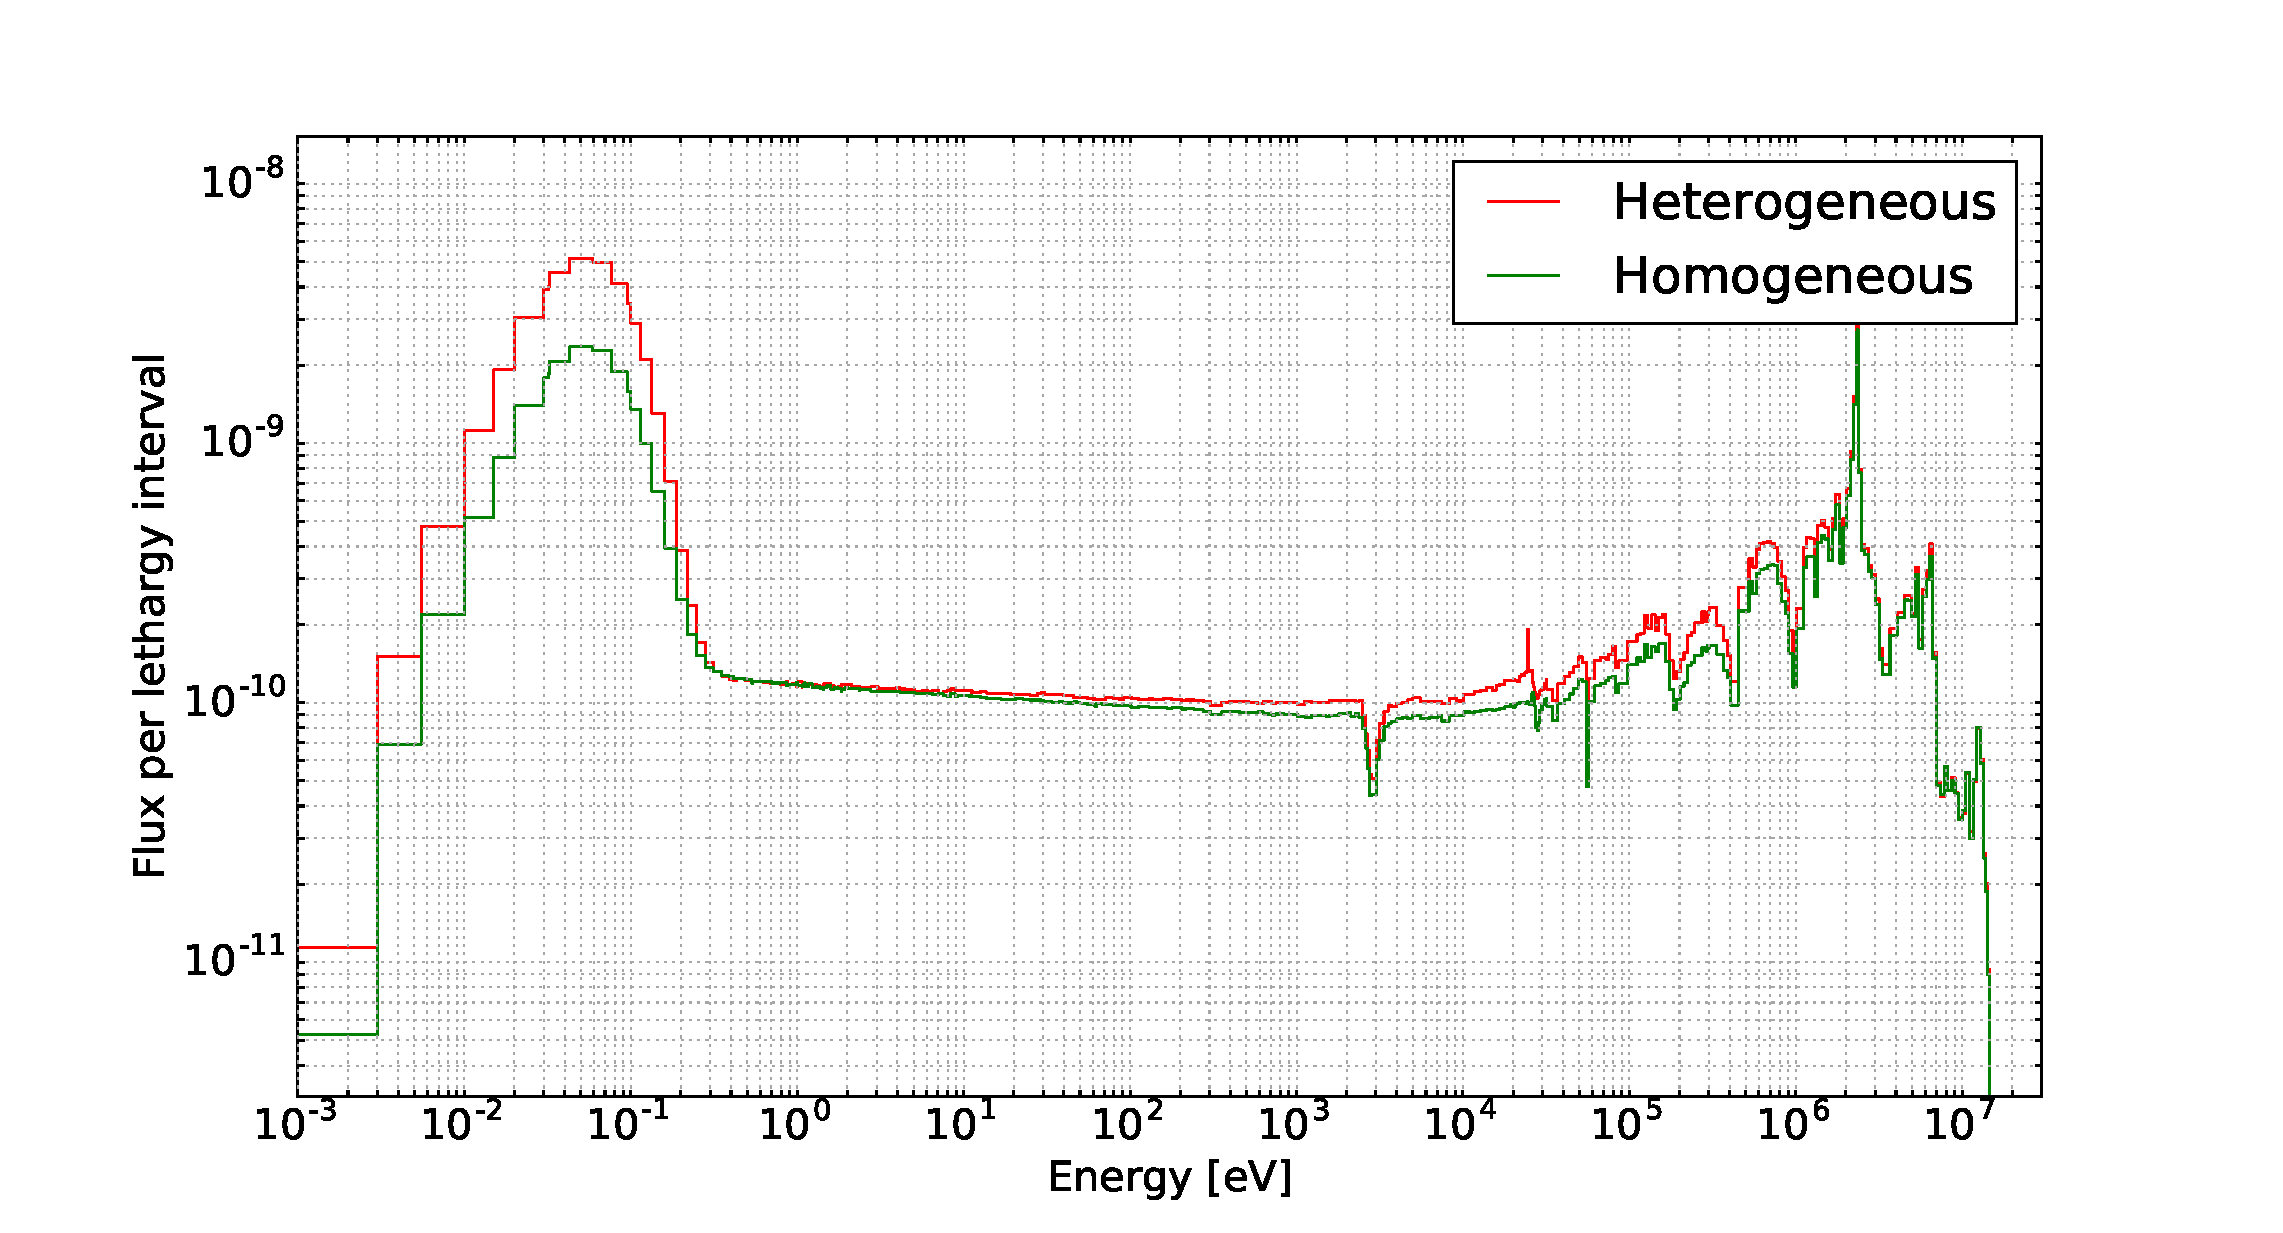
\includegraphics[width=\textwidth]{transmitted_neutron_spectra}
	\caption{The neutron spectra leaving the shield for the heterogeneous and homogeneously modelled cases. Note the substantially reduced thermal flux in the homogeneous simulation. This spectrum has been binned with a finer energy grid than the source, the TRIPOLI 315 group structure.}
	\label{fig:trans_neutron_spec}
\end{figure}

% column span figure
\begin{figure}[H]
  \figuretitle{Radiative capture probability}
  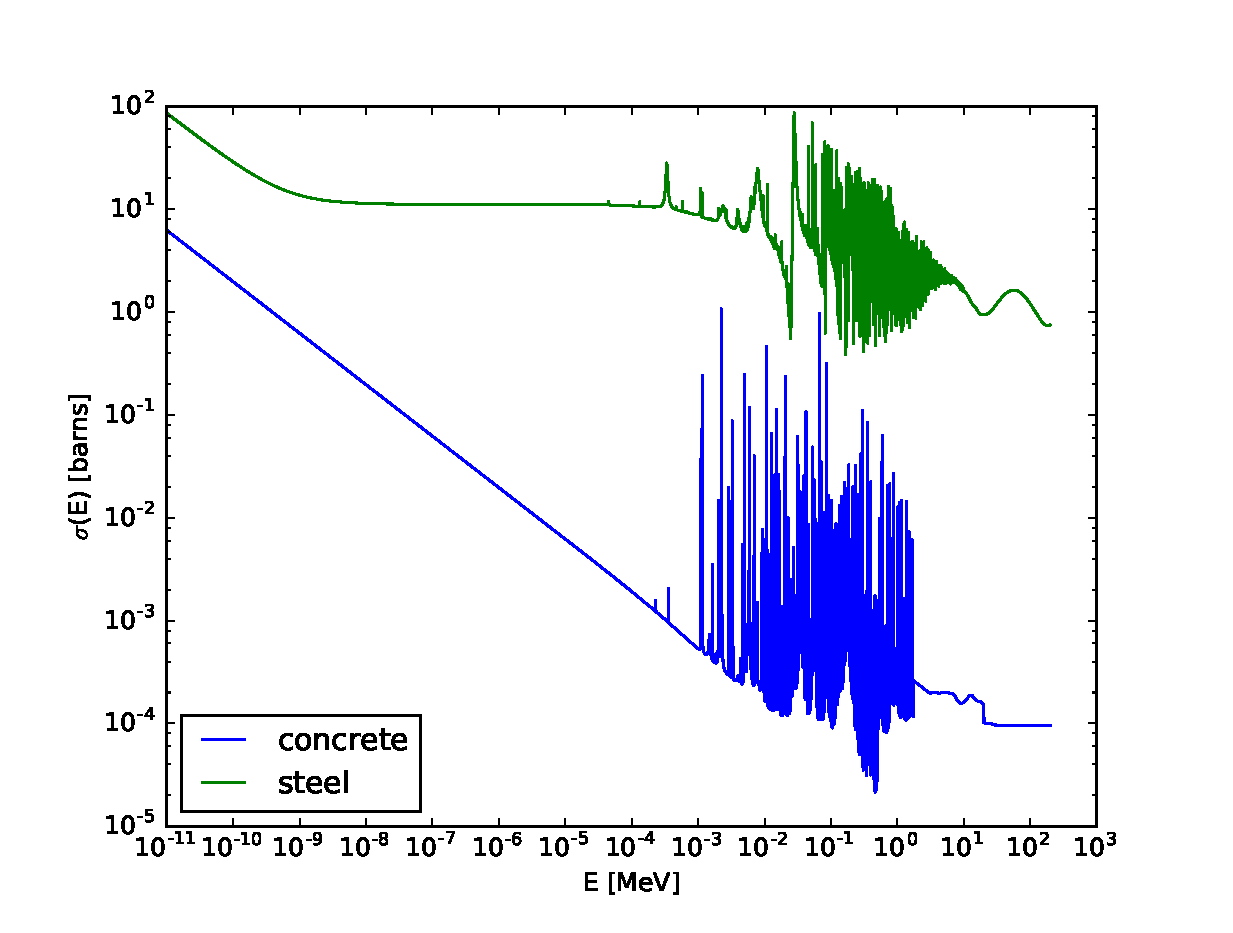
\includegraphics[width=\textwidth]{n_rad_capture}
  \caption{The nuclear properties of steel and concrete are substantially different. Shown here is the cross-section for $(n,\gamma)$ in both materials.}
  \label{fig:n_rad_capture}
\end{figure}

Plotting the ration of the leakage neutron spectra as figure \ref{fig:relative_neutron_spectra} we can see the differences more easily. Thermal flux is underestimated by more than a factor 2. But also, fast flux in the 1keV--1MeV range is underestimated by $\sim1.2$. The fast flux discrepancy is correlated with wall thickness and is negligible for thin (\textless 1m) walls.

% column span figure
\begin{figure}[H]
  \figuretitle{Relative neutron spectra}
	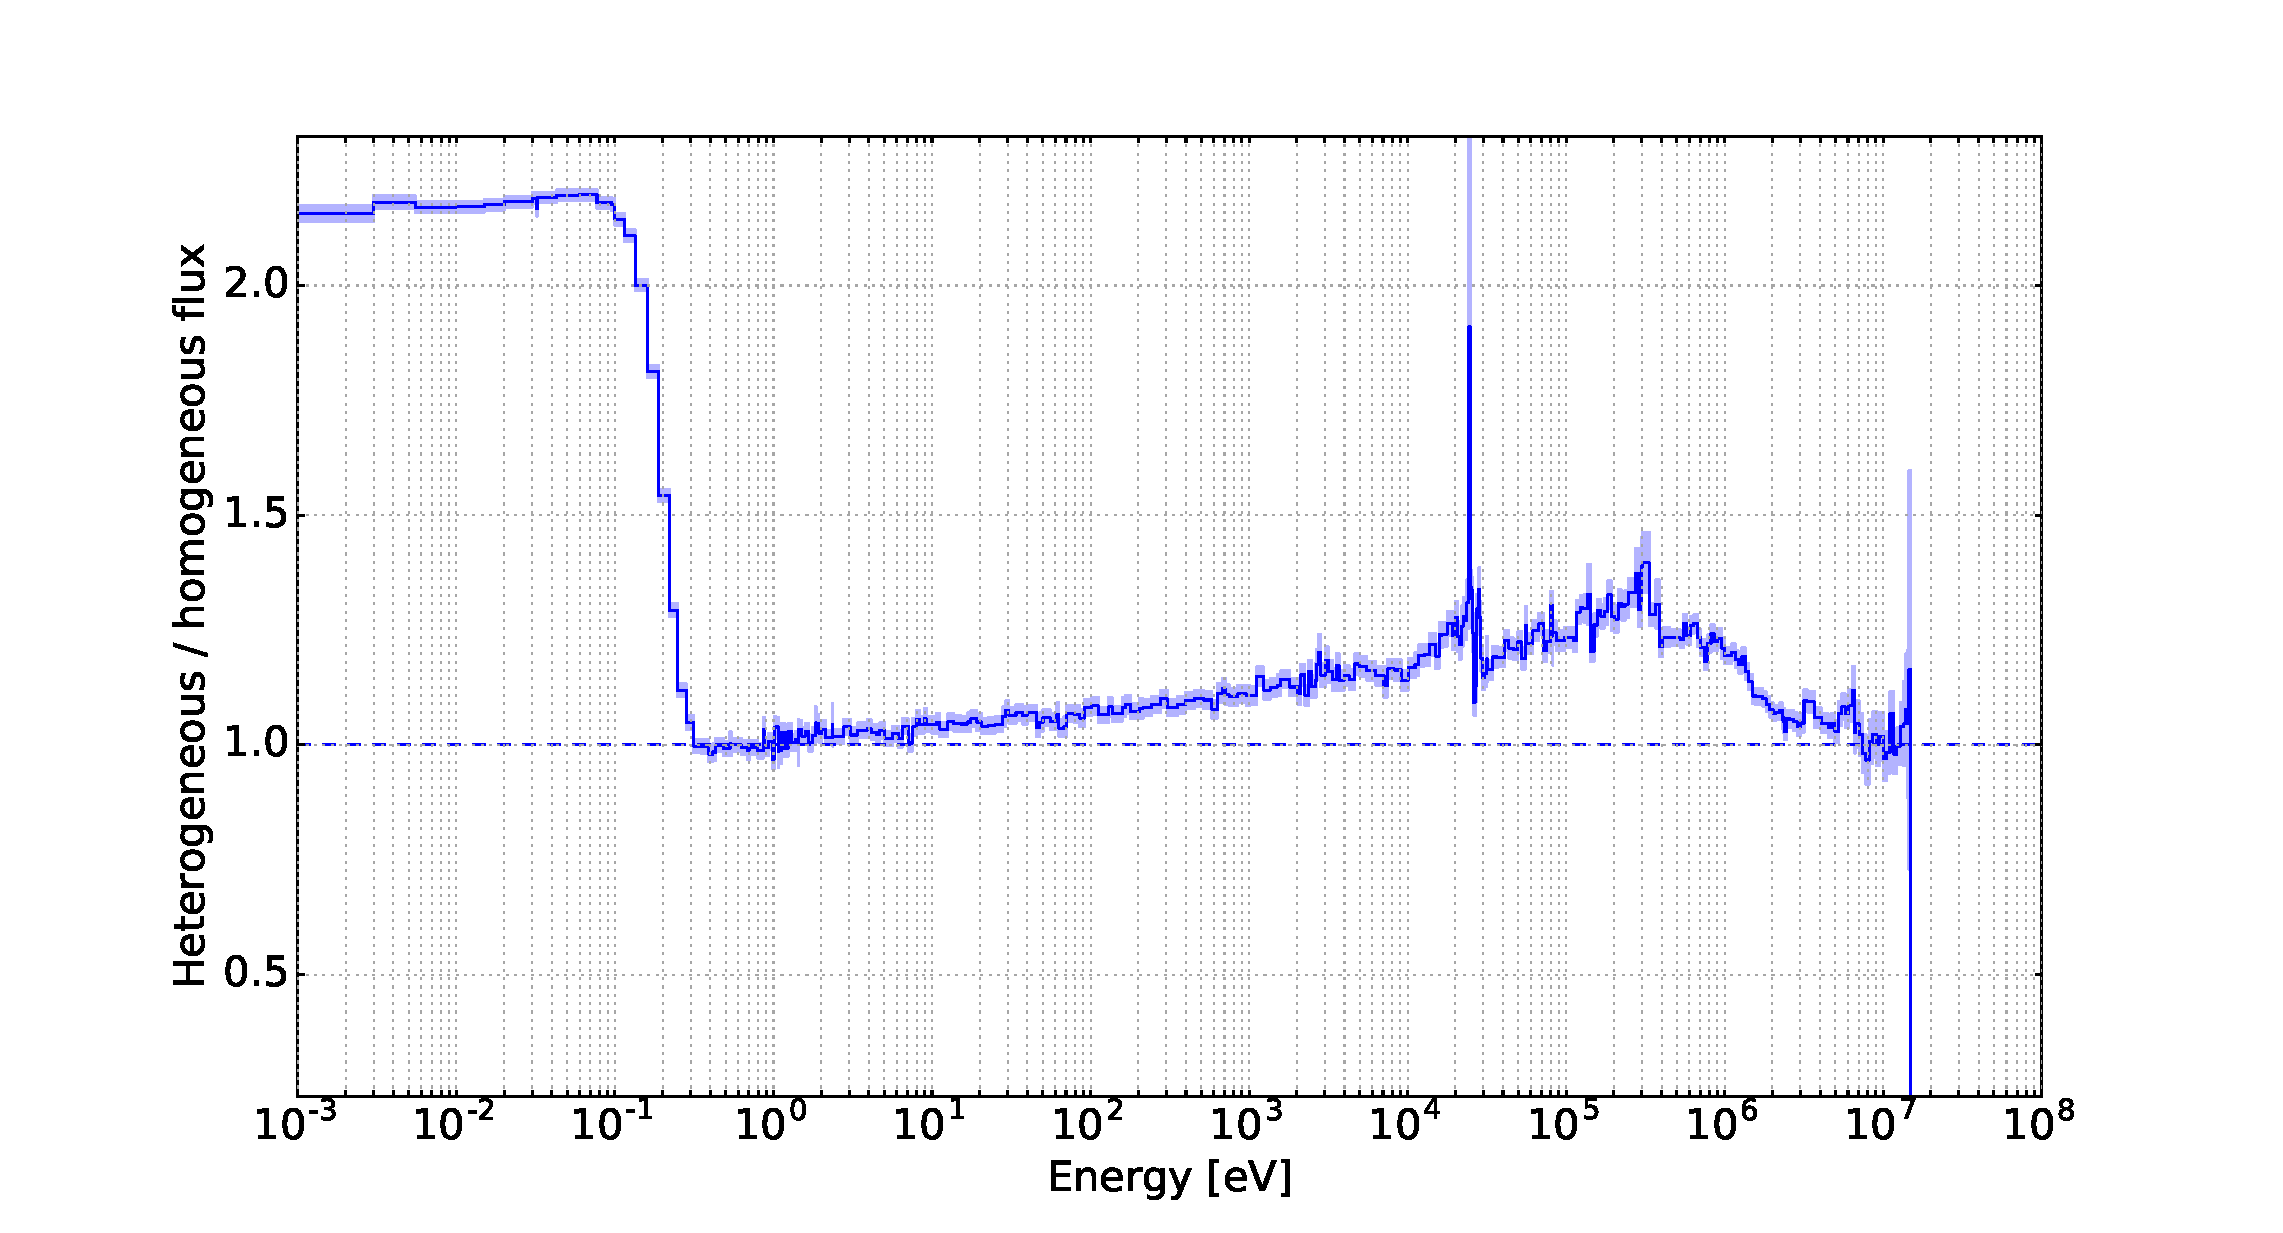
\includegraphics[width=\textwidth]{relative_neutron_spectra}
	\caption{The homogeneous flux increases are readily visible here.}
	\label{fig:relative_neutron_spectra}
\end{figure}

% % column span figure
% \begin{figure}[H]
%   \figuretitle{Contribution to neutron dose}
%   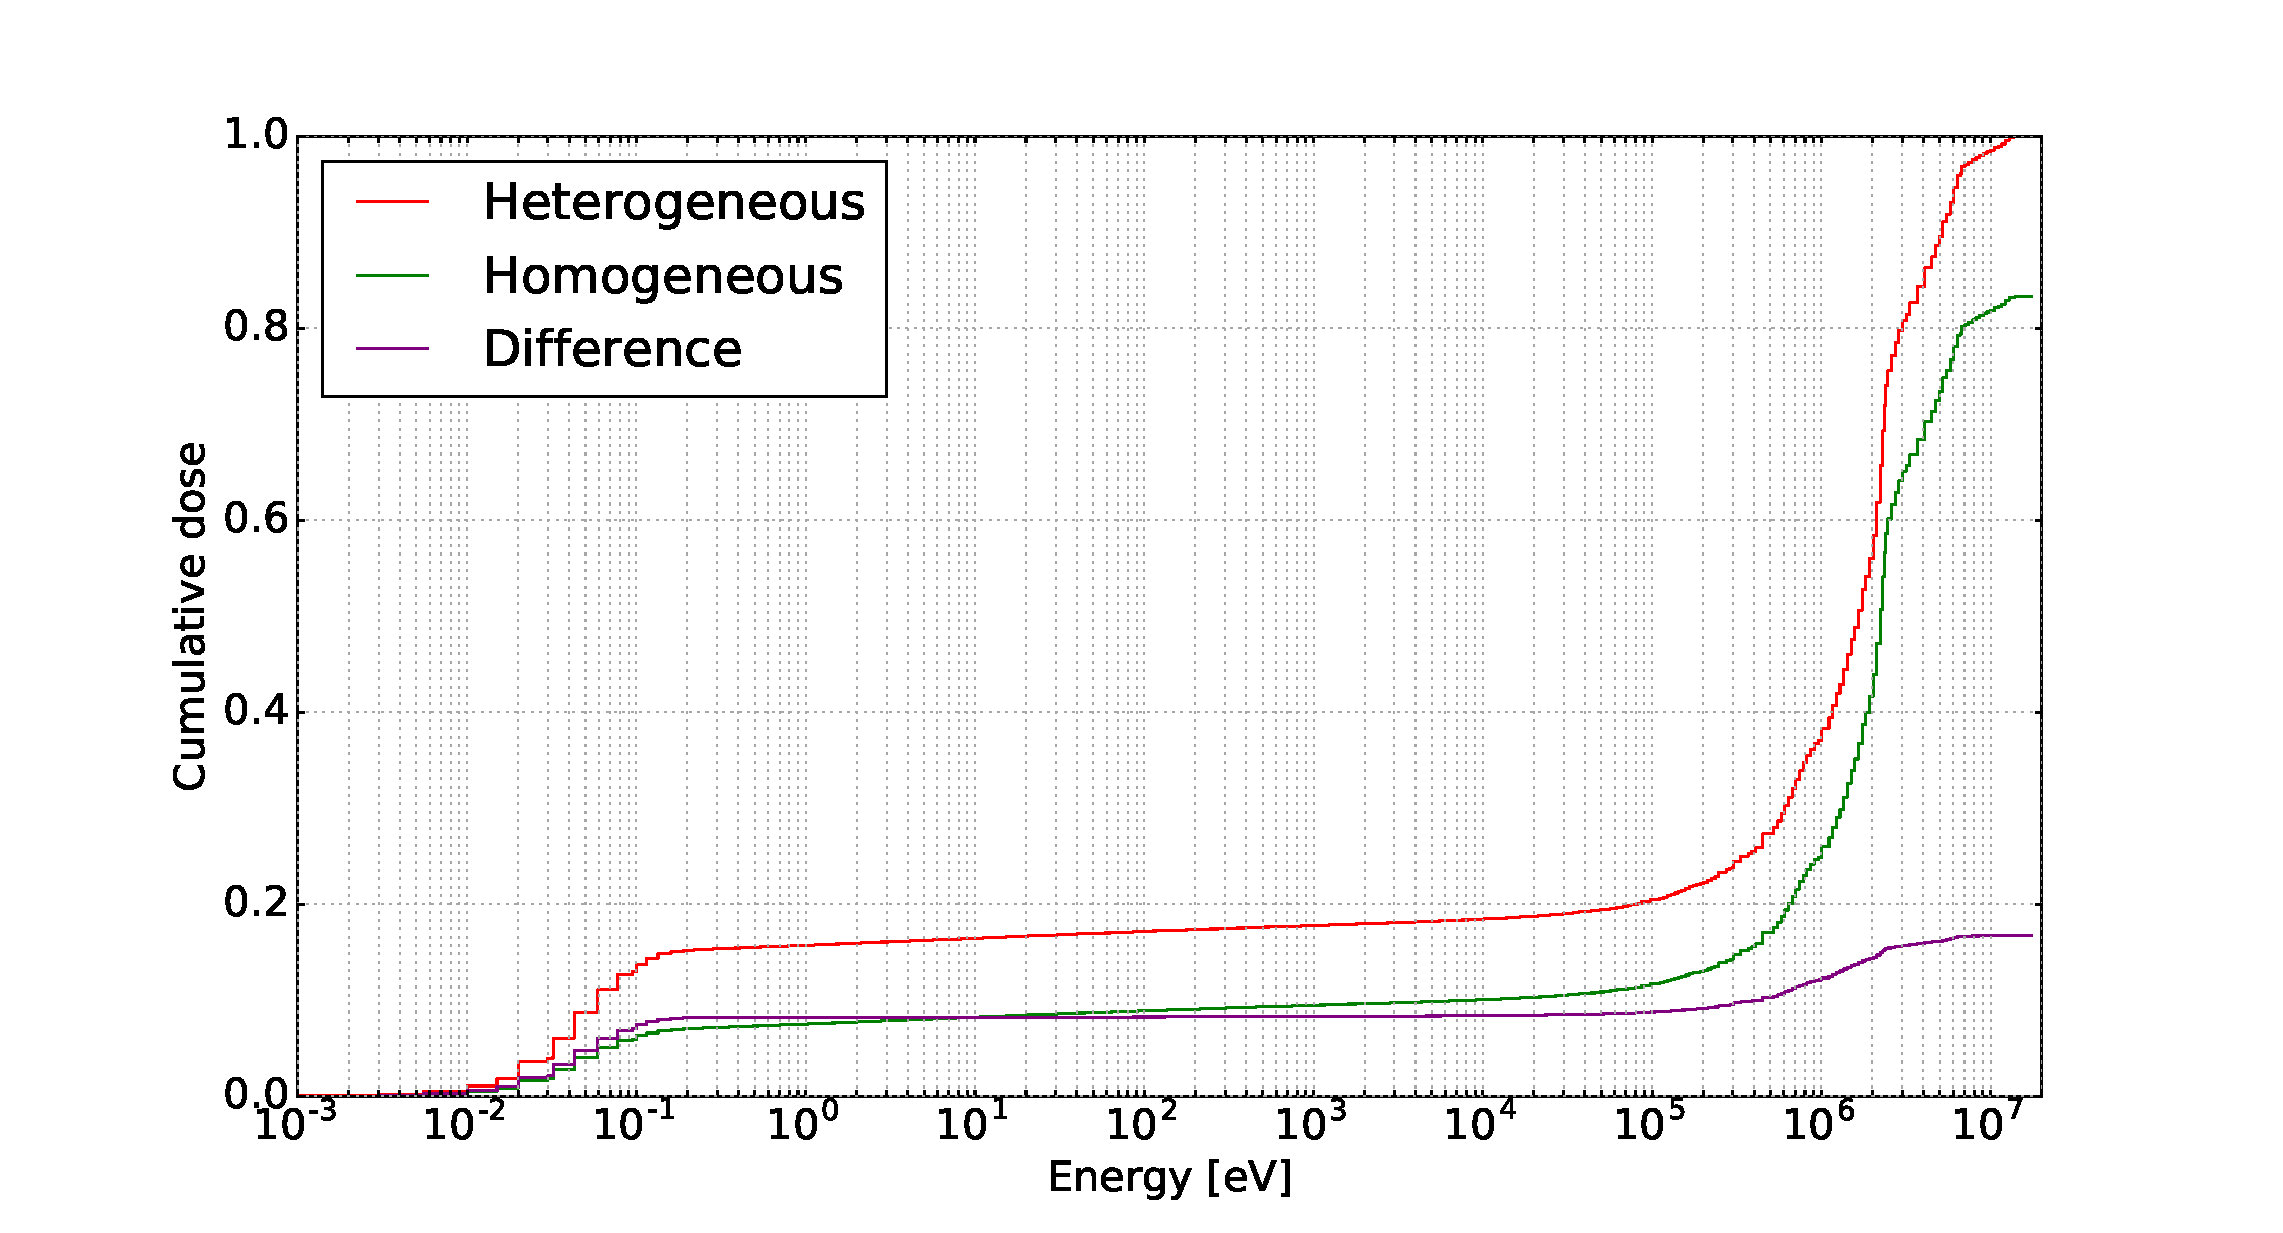
\includegraphics[width=0.5\textwidth]{cumulative_neutron_dose}
%   \caption{Here the dose is cumulatively summed along the energy axis, giving an indication of which energies the dose due to neutrons is from.}
%   \label{fig:cumulative_neutron_dose}
% \end{figure}

Figure \ref{fig:dose_discrepancy} shows how the discrepancy due to the homogeneous approximation varies with wall thickness. It can be seen that the effect is greatest for neutrons. It also plateaus at $\sim 1m$ wall thickness.

% column span figure
\begin{figure}[H]
  \figuretitle{Dose discrepancy due to homogeneity}
	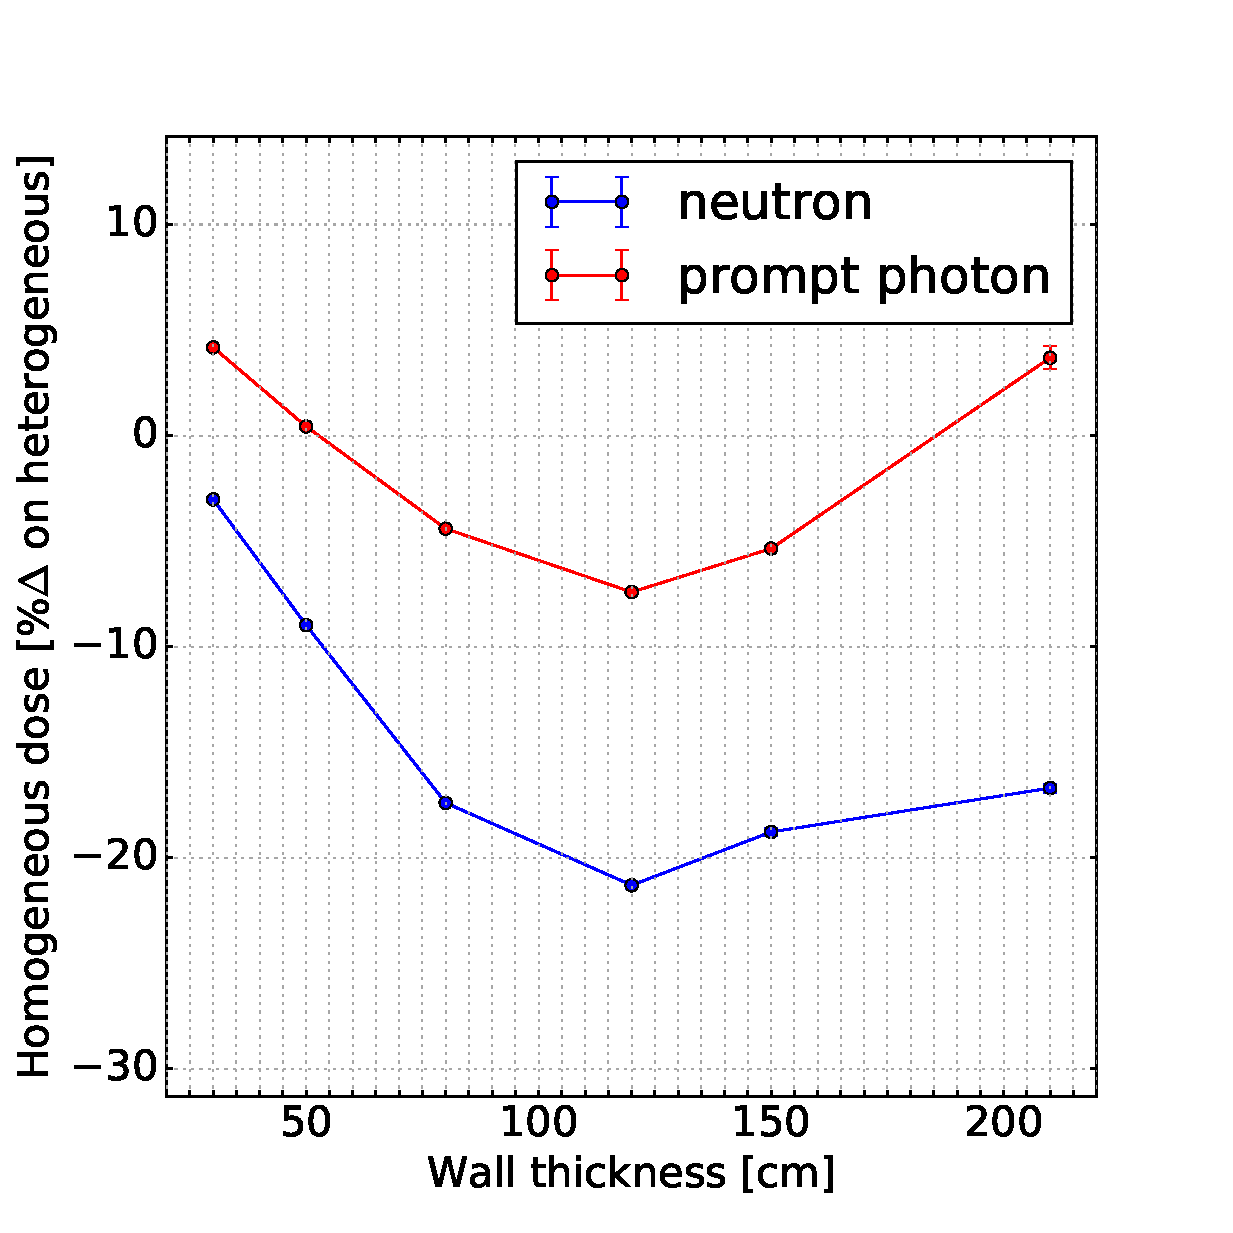
\includegraphics[width=\textwidth]{wall_thickness_dose_discrep}
	\caption{The discrepancy between modelling approaches is a function of the wall thickness for thin walls.}
	\label{fig:dose_discrepancy}
\end{figure}

\subsection{Shut Down Dose Rate}
\label{subsec:sddr}

After operation of a tokamak, repairs and maintenance are often necessary. This section explores the shut-down dose due to be received from the wall itself. It assumes a worker is inside the bioshield at ITER, stood 30cm from the inner surface of an activated wall.\par
Spatial homogenisation acts to overestimate the SDDR beyond 1 day (see figure \ref{fig:sddr}). The homogenised steel in the first few centimeters of the wall is activated by a stronger neutron flux than the physical rebar, located some 5--10cm inside the concrete (the cover depth).

% column span figure
\begin{figure}[H]
  \figuretitle{Shut-down $\phi_{\gamma}$ 30cm from irradiated concrete}
	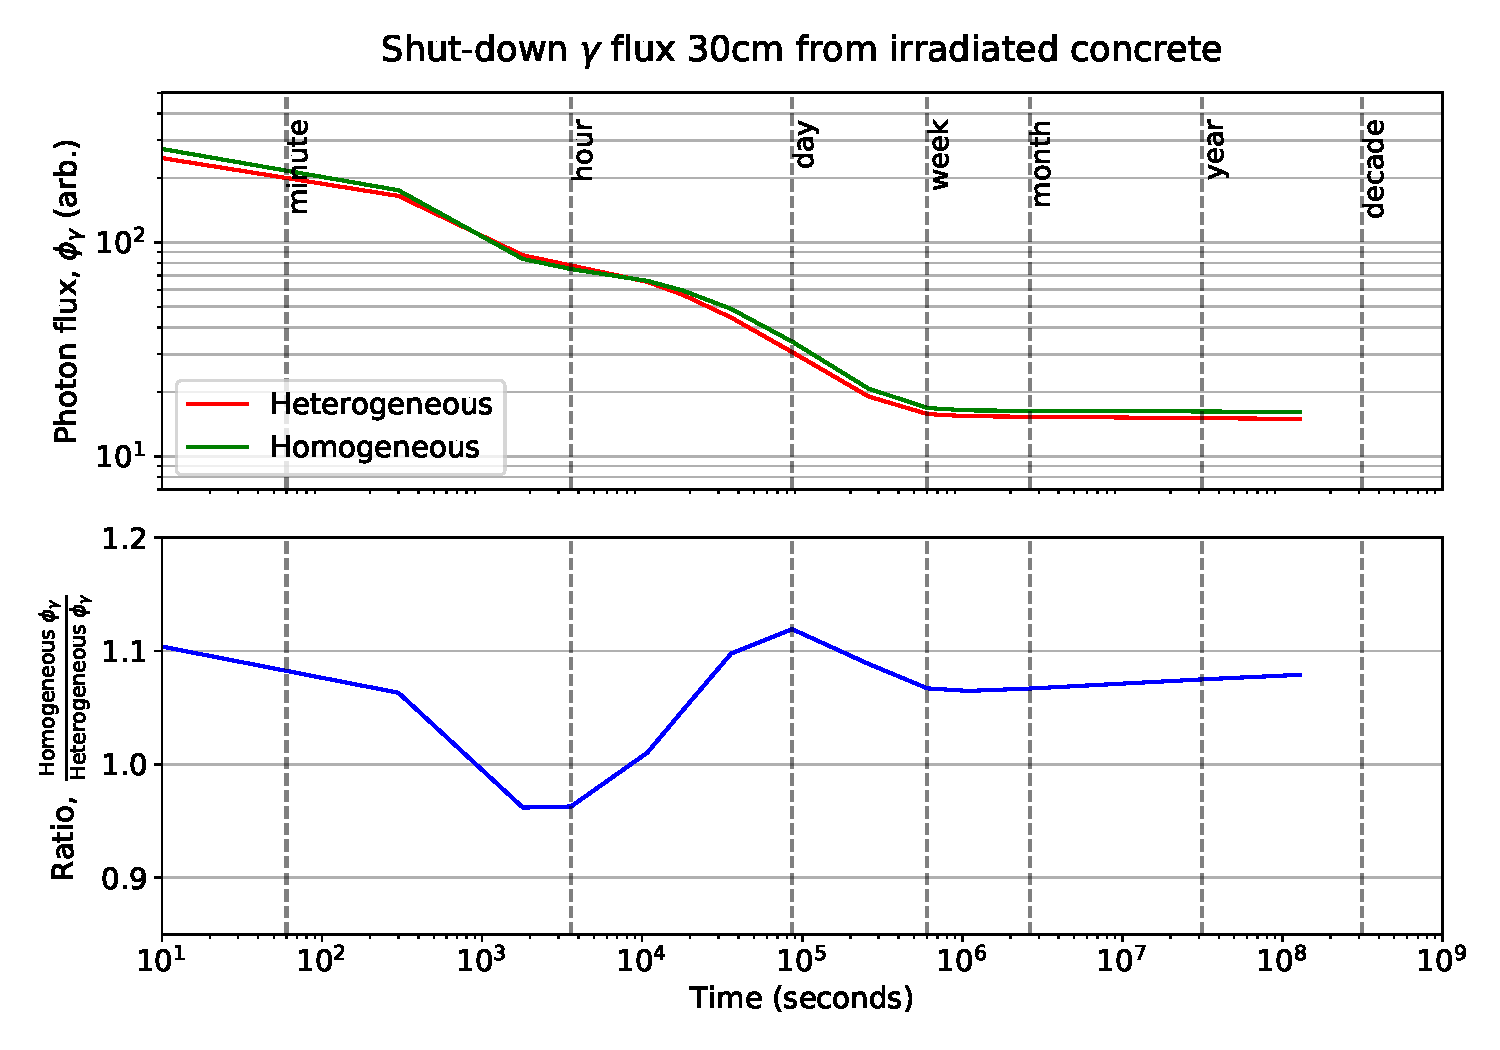
\includegraphics[width=\textwidth]{sddr}
	\caption{The total $\phi_{\gamma}$ as a function of cooling time. The homogeneous simulation gives a significantly increased value at time steps beyond $10^{5}s$ or approximately 1 day.}
	\label{fig:sddr}
\end{figure}

The mean free path of neutrons near the surface is $\sim2cm$ (see figure \ref{fig:mfp}) and as such a typical neutron will undergo several collisions before arriving at the rebar in a heterogeneous simulation. However, in a homogeneous simulation a small amount of steel is present right at the very surface of the concrete, as it is present throughout the simulation. This steel is exposed to an intense neutron flux and is activated accordingly.

% column span figure
\begin{figure}[H]
  \figuretitle{Neutron path length in concrete}
	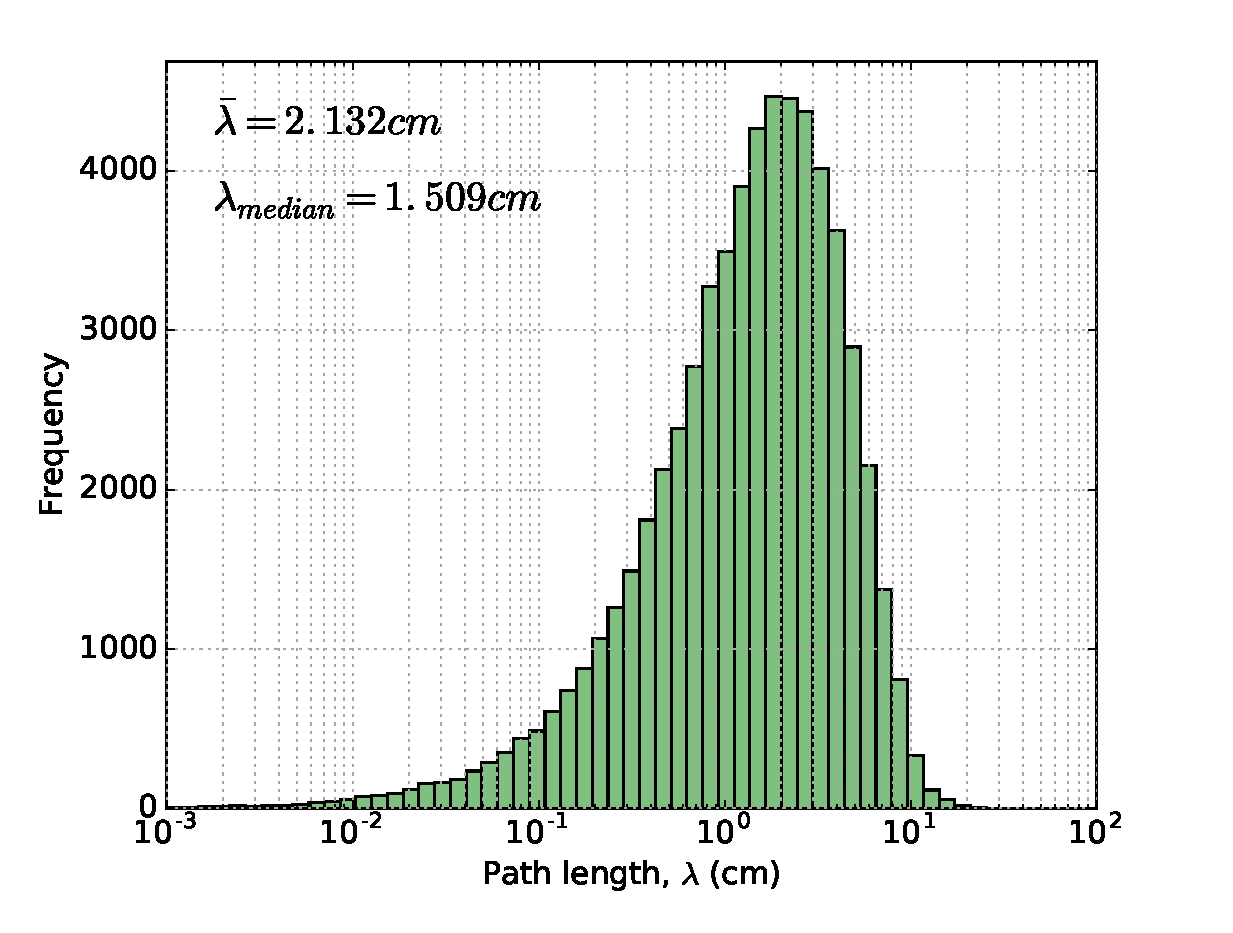
\includegraphics[width=\textwidth]{mfp}
	\caption{The path lengths of neutrons in pure concrete are shown as a histogram. There is a wide distribution with a mean of approximately 2cm.}
	\label{fig:mfp}
\end{figure}

The plot shown as figure \ref{fig:contact_dose} is produced with data from the activation solver FISPACT-II. Shown are estimates for a contact dose with concrete and steel. As the steel is buried within concrete, the numbers plotted here are not a substitute for transporting decay $\gamma$ photons from their birth to their death. However, they do give a good feel for which nuclides are responsible for the activity of a material at a given time. It is clear that after $^{28}$Al and $^{24}$Na decay in concrete, it has become substantially less active. It is around this time that steel becomes the dominant contributor to dose and the homogeneous modelling approach diverges from heterogeneous.

% column span figure
\begin{figure}[H]
  \figuretitle{Contact dose rate by material}
  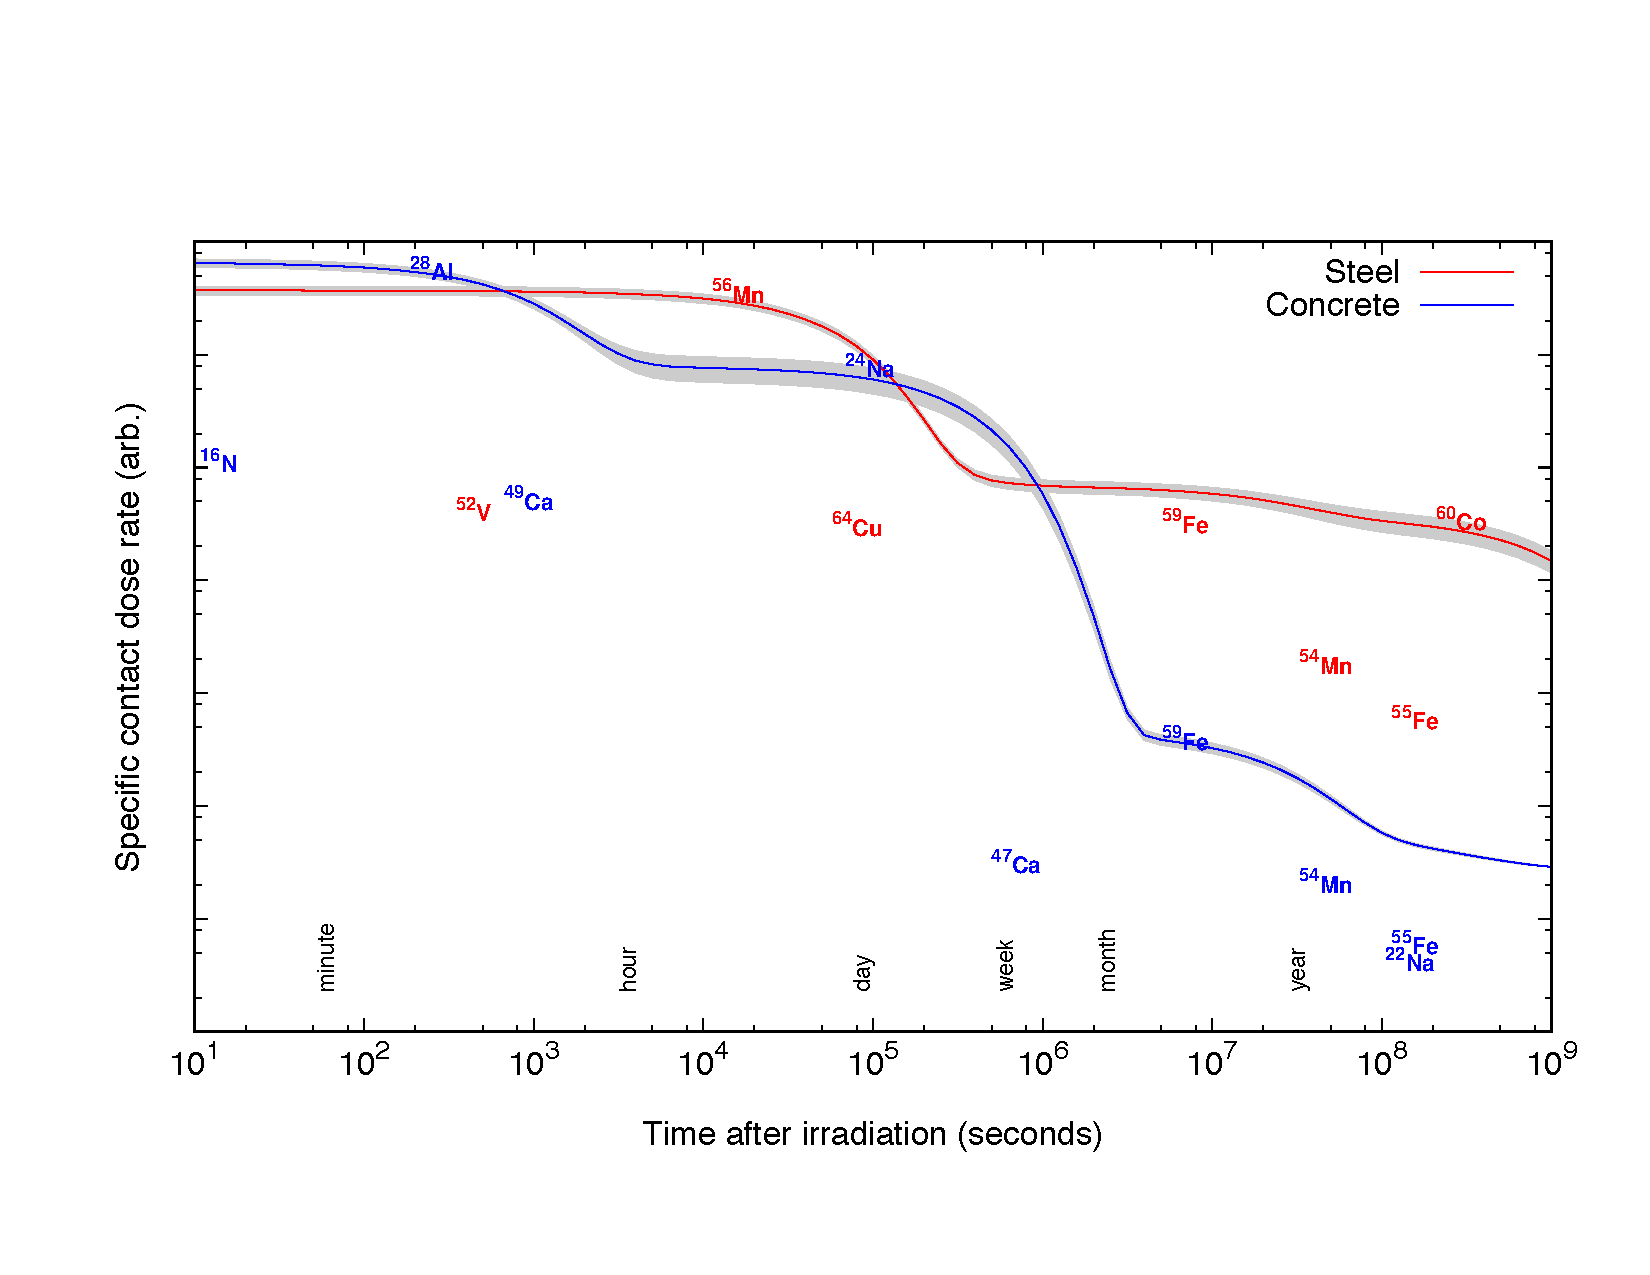
\includegraphics[width=\textwidth]{contact_dose_by_mat}
	\caption{This plot shows an estimate for the specific contact dose rate due to steel and concrete irradiated under the ITER SA-2 scenario. Nuclides which contribute a significant fraction of the dose are shown with their abscissa value as their half-life, $t_{\frac{1}{2}}$.}
	\label{fig:contact_dose}
\end{figure}

% % page span figure
% \end{multicols}
% \begin{figure}[H]
%   \begin{center}
%     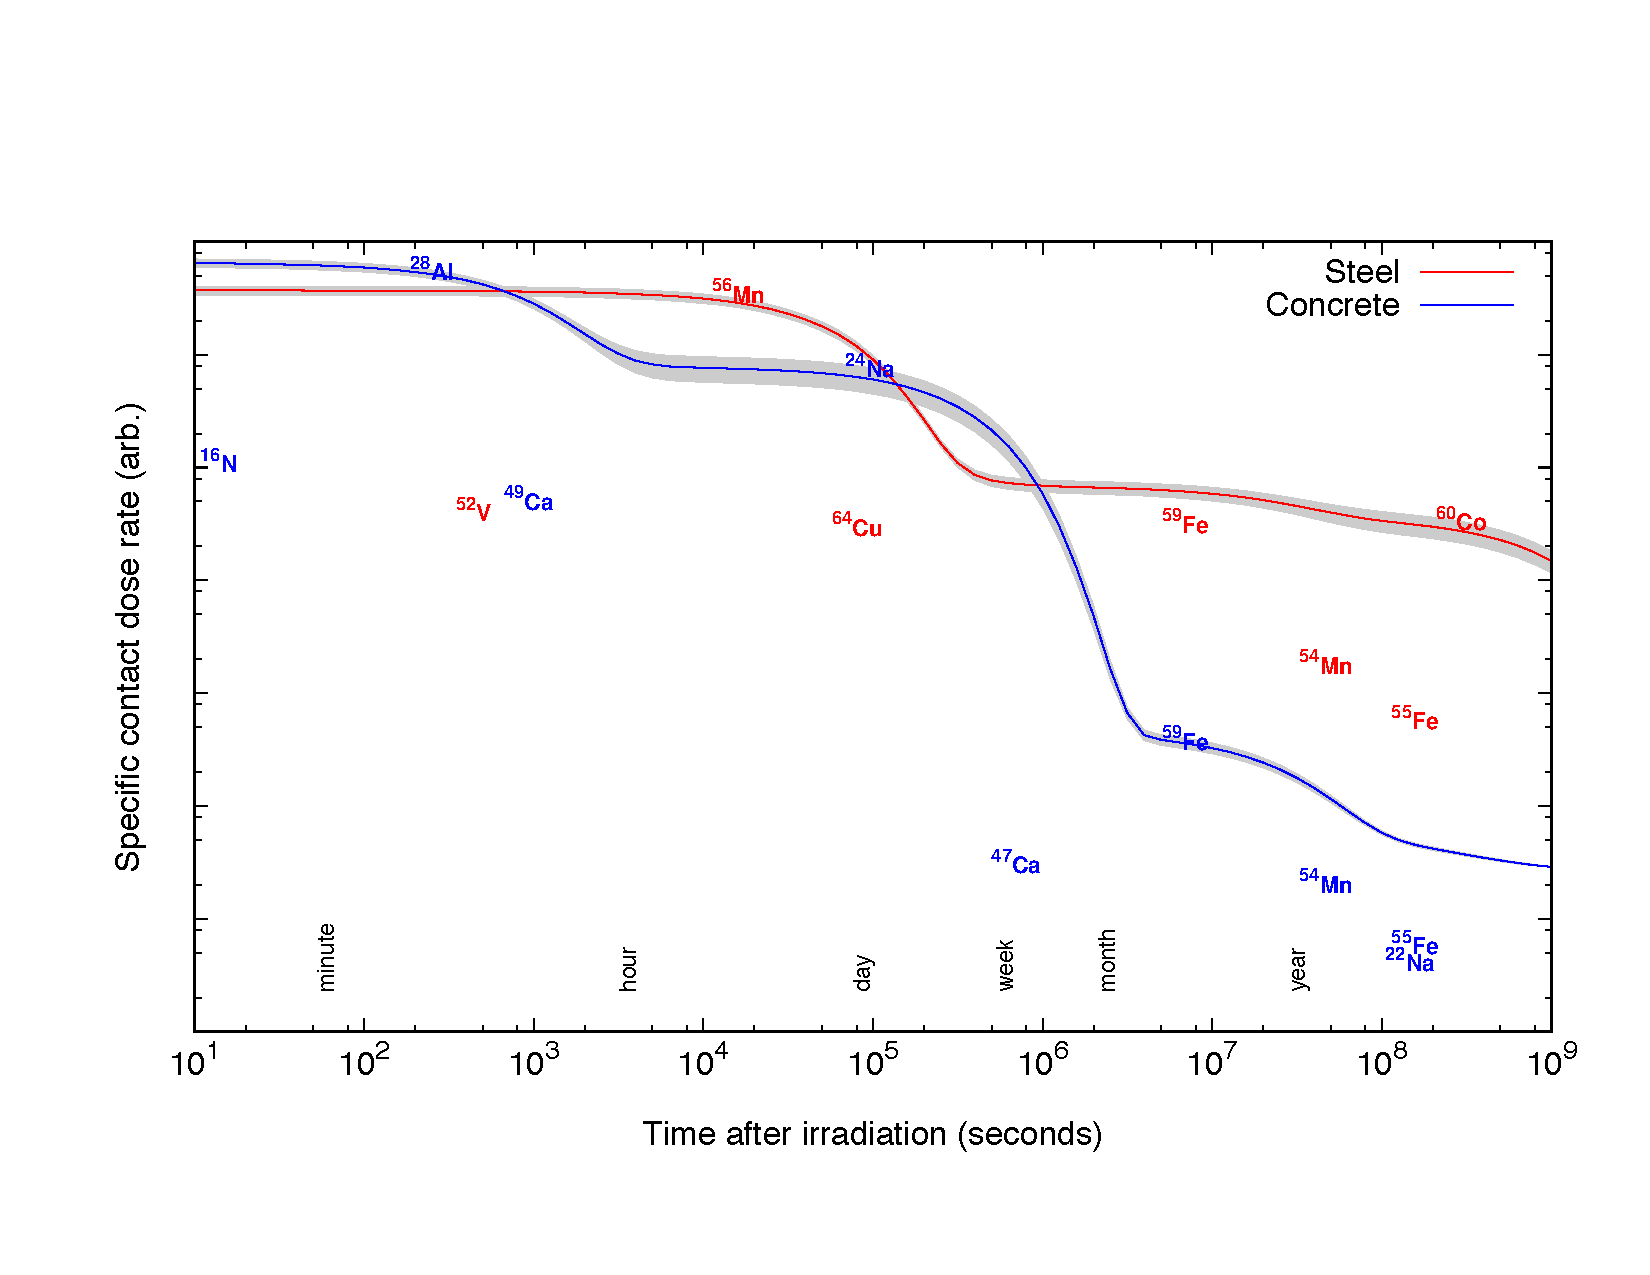
\includegraphics[width=0.8\textwidth]{contact_dose_by_mat}
%   \end{center}
%   \caption{This plot shows an estimate for the specific contact dose rate due to steel and concrete irradiated under the ITER SA-2 scenario. Nuclides which contribute a significant fraction of the dose are marked.}
%   \label{fig:contact_dose}
% \end{figure}
% \begin{multicols}{2}

\section{Conclusion}
The spatial homogenisation modelling approximation for reinforced concrete underestimates the dose due to neutrons by up to 20\%. The dose due to on-load photons can be underestimated by up to 8\%.\par
The SDDR is instead overestimated by homogenisation, by up to a factor 60 at times beyond a day. 

%!TEX root = ../thesis.tex
%*******************************************************************************
%****************************** Third Chapter **********************************
%*******************************************************************************
\chapter{Optimising energy group structures for neutron activation calculations in fusion systems}
\label{chap:group_structure}

% **************************** Define Graphics Path **************************
\ifpdf
    \graphicspath{{Chapter3/Figs/Raster/}{Chapter3/Figs/PDF/}{Chapter3/Figs/}}
\else
    \graphicspath{{Chapter3/Figs/Vector/}{Chapter3/Figs/}}
\fi

% INTRODUCTION
%   Group structure optimisation literature review
%     Include a simple convergence study result
%   Self-shielding
%   Resonance behaviour: parameter correlations (matrix, resonance widths, f(Z,E))
%     Resonance Integrals, although structure, big resonances spread out over E-space
% METHOD
%   Nuclear data processing infrastructure
%     Pointwise ENDF
%     A Compact ENDF
%     Groupwise ENDF
%     Probability tables
%     Self-shielding factors
%   Energy group optimisation
%     Building a bin density distribution: rho(E) = SSF_{eff} + bpd_min
%     An iterative implementation
%   Radiation transport
%     Simple test case    # data on freia
%     JET model           
% RESULTS
%   Single optimisation: JET activation foils
%   Iterative optimisation: simple test case
% CONCLUSIONS / FURTHER WORK

\section{Outline}
\label{sec:outline}
% Update this

This study utilises self-shielding factors as a means to optimise energy group structures for fusion activation calculations. Informed by an analysis of important fusion resonances and a survey of relevant incident particle spectra, we develop and test two new group structures designed to more accurately represent the physics of nuclear reactions. They are compared to group structures commonly used in fusion research \& analysis. When used in a JET activation foil scenario, the optimised group structures outperform reference group structures, such as CCFE-709, while requiring fewer bins.

\section{Introduction}

Nuclear simulations for fusion devices are essential to determine material damage, activation-transmutation and to perform dose rate analyses. While continuous energy Monte Carlo modeling can be used to directly calculate reaction rates, due to the very large number (potentially tens of thousands) of possible reaction channels, it is impractical to compute all nuclear reactions of interest by this so-called point-wise approach. A separate inventory code, such as FISPACT-II \cite{fispact2015}, utilising a discretised incident particle spectrum is typically used to calculate all of these reaction rates, solve for the time-dependent nuclide inventory and provide various responses and source terms. This multi-group method is computationally efficient, but introduces self-shielding errors.

\subsection{Group structure optimisation}
% Greatly expand this...
The likelihood of interaction between an incident particle and a nucleus is a a non-linear function of energy in the resonant energy region. The cross-section, $\sigma(\mathrm{E})$ and the associated reaction rate, RR(E), may vary by several orders of magnitude within a few electron-volts. The number of bins that the energy domain is discretised over has a strong influence on the accuracy of the result. While increasing the number of bins increases the accuracy it also increases the time required to converge an input spectrum and the memory required to record this information\footnote{A concern for simulations with millions of voxels, common in activation-dose calculations.}. Figure~\ref{fig:gendf_convergence} shows a reaction rate converging to the true result as a function of the number of cross-section groups. These results are from a simple model where a 14 MeV point neutron source is located within a series of concentric, spherical shells made of steel, water and tungsten. The tallied reaction rate is radiative capture in \textsuperscript{186} in the outermost, tungsten shell. The neutrons are moderated by the water and the energy spectrum will receive sharp flux depressions from resonant nuclides within the steel material. This flux is then incident upon the tungsten where resonant peaks from the tungsten isotopes will further impinge on the spectrum. Without adequately resolving these depressions, an accurate estimation of the desired reaction rate cannot be made. In this example it can be seen that getting from a 10\% error to $\approx 1\%$ error requires a jump from 256 to more than 8192 bins. Any real problem will have many hundreds of nuclides present, with their nuclear data all discretised the same way, whether for a deterministic radiation transport calculation or an activation-transmutation calculation. Adopting such a fine discretisation for so many nuclides is not feasible given the memory requirements of such a scheme.

\begin{figure}[H]
  \centering
  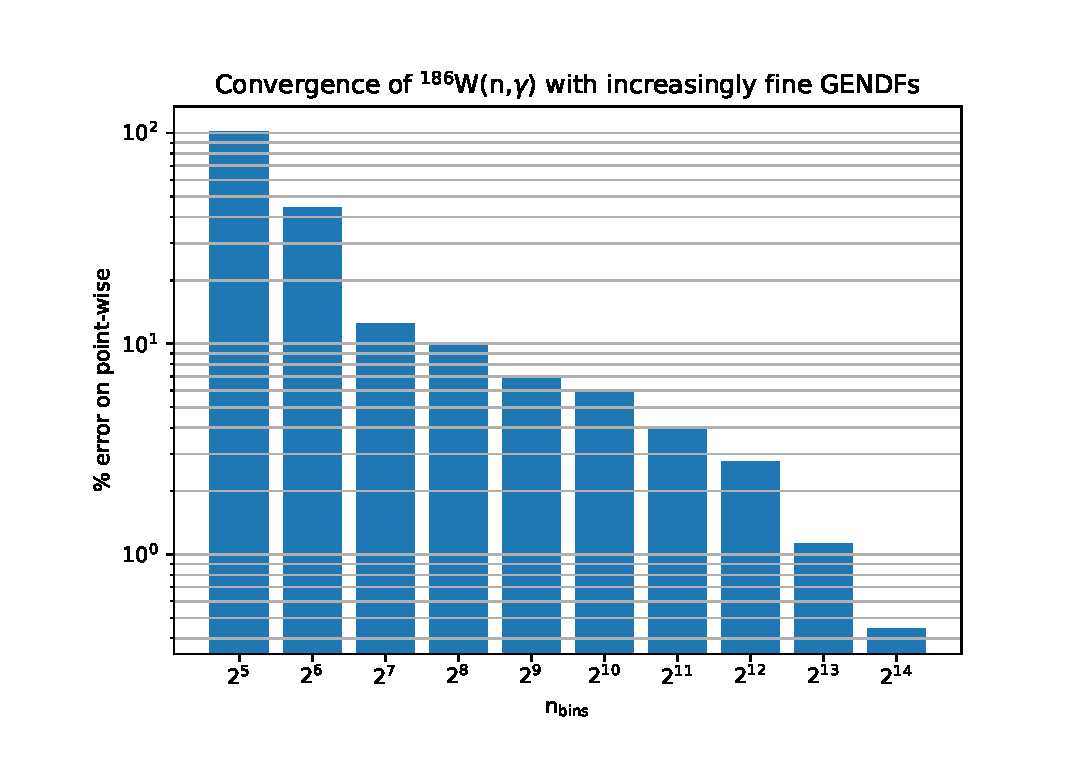
\includegraphics[width=0.9\linewidth]{gendf_convergence}
  \caption{This figure shows the results from a series of calculations with increasingly fine energy discretisations, or group structures. The bins for all groups are equally log-spaced. The calculation is to determine the (n,$\gamma$) reaction rate in a shell of \textsuperscript{186}W due to some incident neutron flux. The dependent variable is the \% change on a point-wise (true) value calculated with MCNP.}
  \label{fig:gendf_convergence}
\end{figure}

In addition to the number of bins, the bound locations have a strong relationship to the result accuracy. The integer bin count number and bound locations energy vector are together known as an energy group structure. In the example shown in figure~\ref{fig:gendf_convergence} the bin boundaries have been uniformally logarithmically distributed. This is a very simple starting point (and many group structures largely adhere to it) and can be improved upon, even if only to adopt one or two regions of different bin density.

% Expand this section, giving detail on each method
There have been several previous efforts to optimise neutron energy group structures. Certain applications lend themselves to highly targeted group structures. For example, fission reactor lattice physics calculations are typically interested in determining a few reaction rates to very high accuracy. The Studsvik team who develop the CASMO-5 lattice physics code employ a neutron group structure with very fine resolution around the principal $^{238}\mathrm{U}$ and $^{240}\mathrm{Pu}$ resonances \cite{Rhodes2006}. Covering these areas with a fine energy grid results in a more accurate estimate of key reaction rates and hence calculation of the neutrons absorbed and consequently lost from the system. Particle Swarm Optimisation (PSO) has been used multiple times to improve bin bound placement for multi-group libraries used for reactor physics applications \cite{Yi2013} \cite{Akbari2012} \cite{Akbari2013} \cite{Fleming2016}. \citet{Morgan2013} have explored hyperfine multi-group (MG) data as an alternative to the interpolation of point-wise (PW) data as typically employed by particle transport codes such as MCNP6.1 \cite{goorley2012}. Some attention has been directed towards the refinement of reaction rate calculation for specific elements and nuclides in fusion scenarios. For instance, work on the spatial heterogeneity of tungsten transmutation has been undertaken by \citet{Gilbert2016} who used the CCFE 709 bin group structure and careful application of self-shielding factors to accurately determine reaction rates.
% Comment on whether group structures are general or for specific applications. Can a general one ever be `optimised'? A: It is always a trade-off, generality vs. accuracy.

\subsection{Resonance behaviour}
% In terms of targeting group structure resolution, what can we learn from the distribution of resonance locations and widths?
It is clear that the placement of bin boundaries and the number of bins in an energy group structure has a significant effect on the potential accuracy of any calculation employing that group structure. The ideal location of these bin bounds is not some equal spacing, but more likely some complex result influenced by the kind of spectrum encountered and the nuclei present in the problem. This latter consideration can be explored by analysing the distributions of nuclear resonances for known nuclides within the \{A,E,j,$\Gamma$\} space, where A = atomic mass, $\mathrm{E}_{r}$ = interaction energy, j = nuclear spin and $\Gamma$ = resonance width. With knowledge of these distributions, especially in the mass and energy domains, perhaps energy bins might be targeted intelligently for a given problem.

To undertake this study, a set of scripts were written to parse resonance parameter information from nuclear data libraries. These can read ENDF-6 formatted entries, including several resonance formalisms for maximum nuclide coverage. The nuclear data library chosen to study was ENDF/B-VII.1 \cite{Chadwick2011}, the United States' reference nuclear data library. Figure~\ref{fig:res_energy_mass} is a scatter plot of 41,112 nuclear resonances from nuclides contained within this libary. 

\begin{figure}[H]
  \centering
  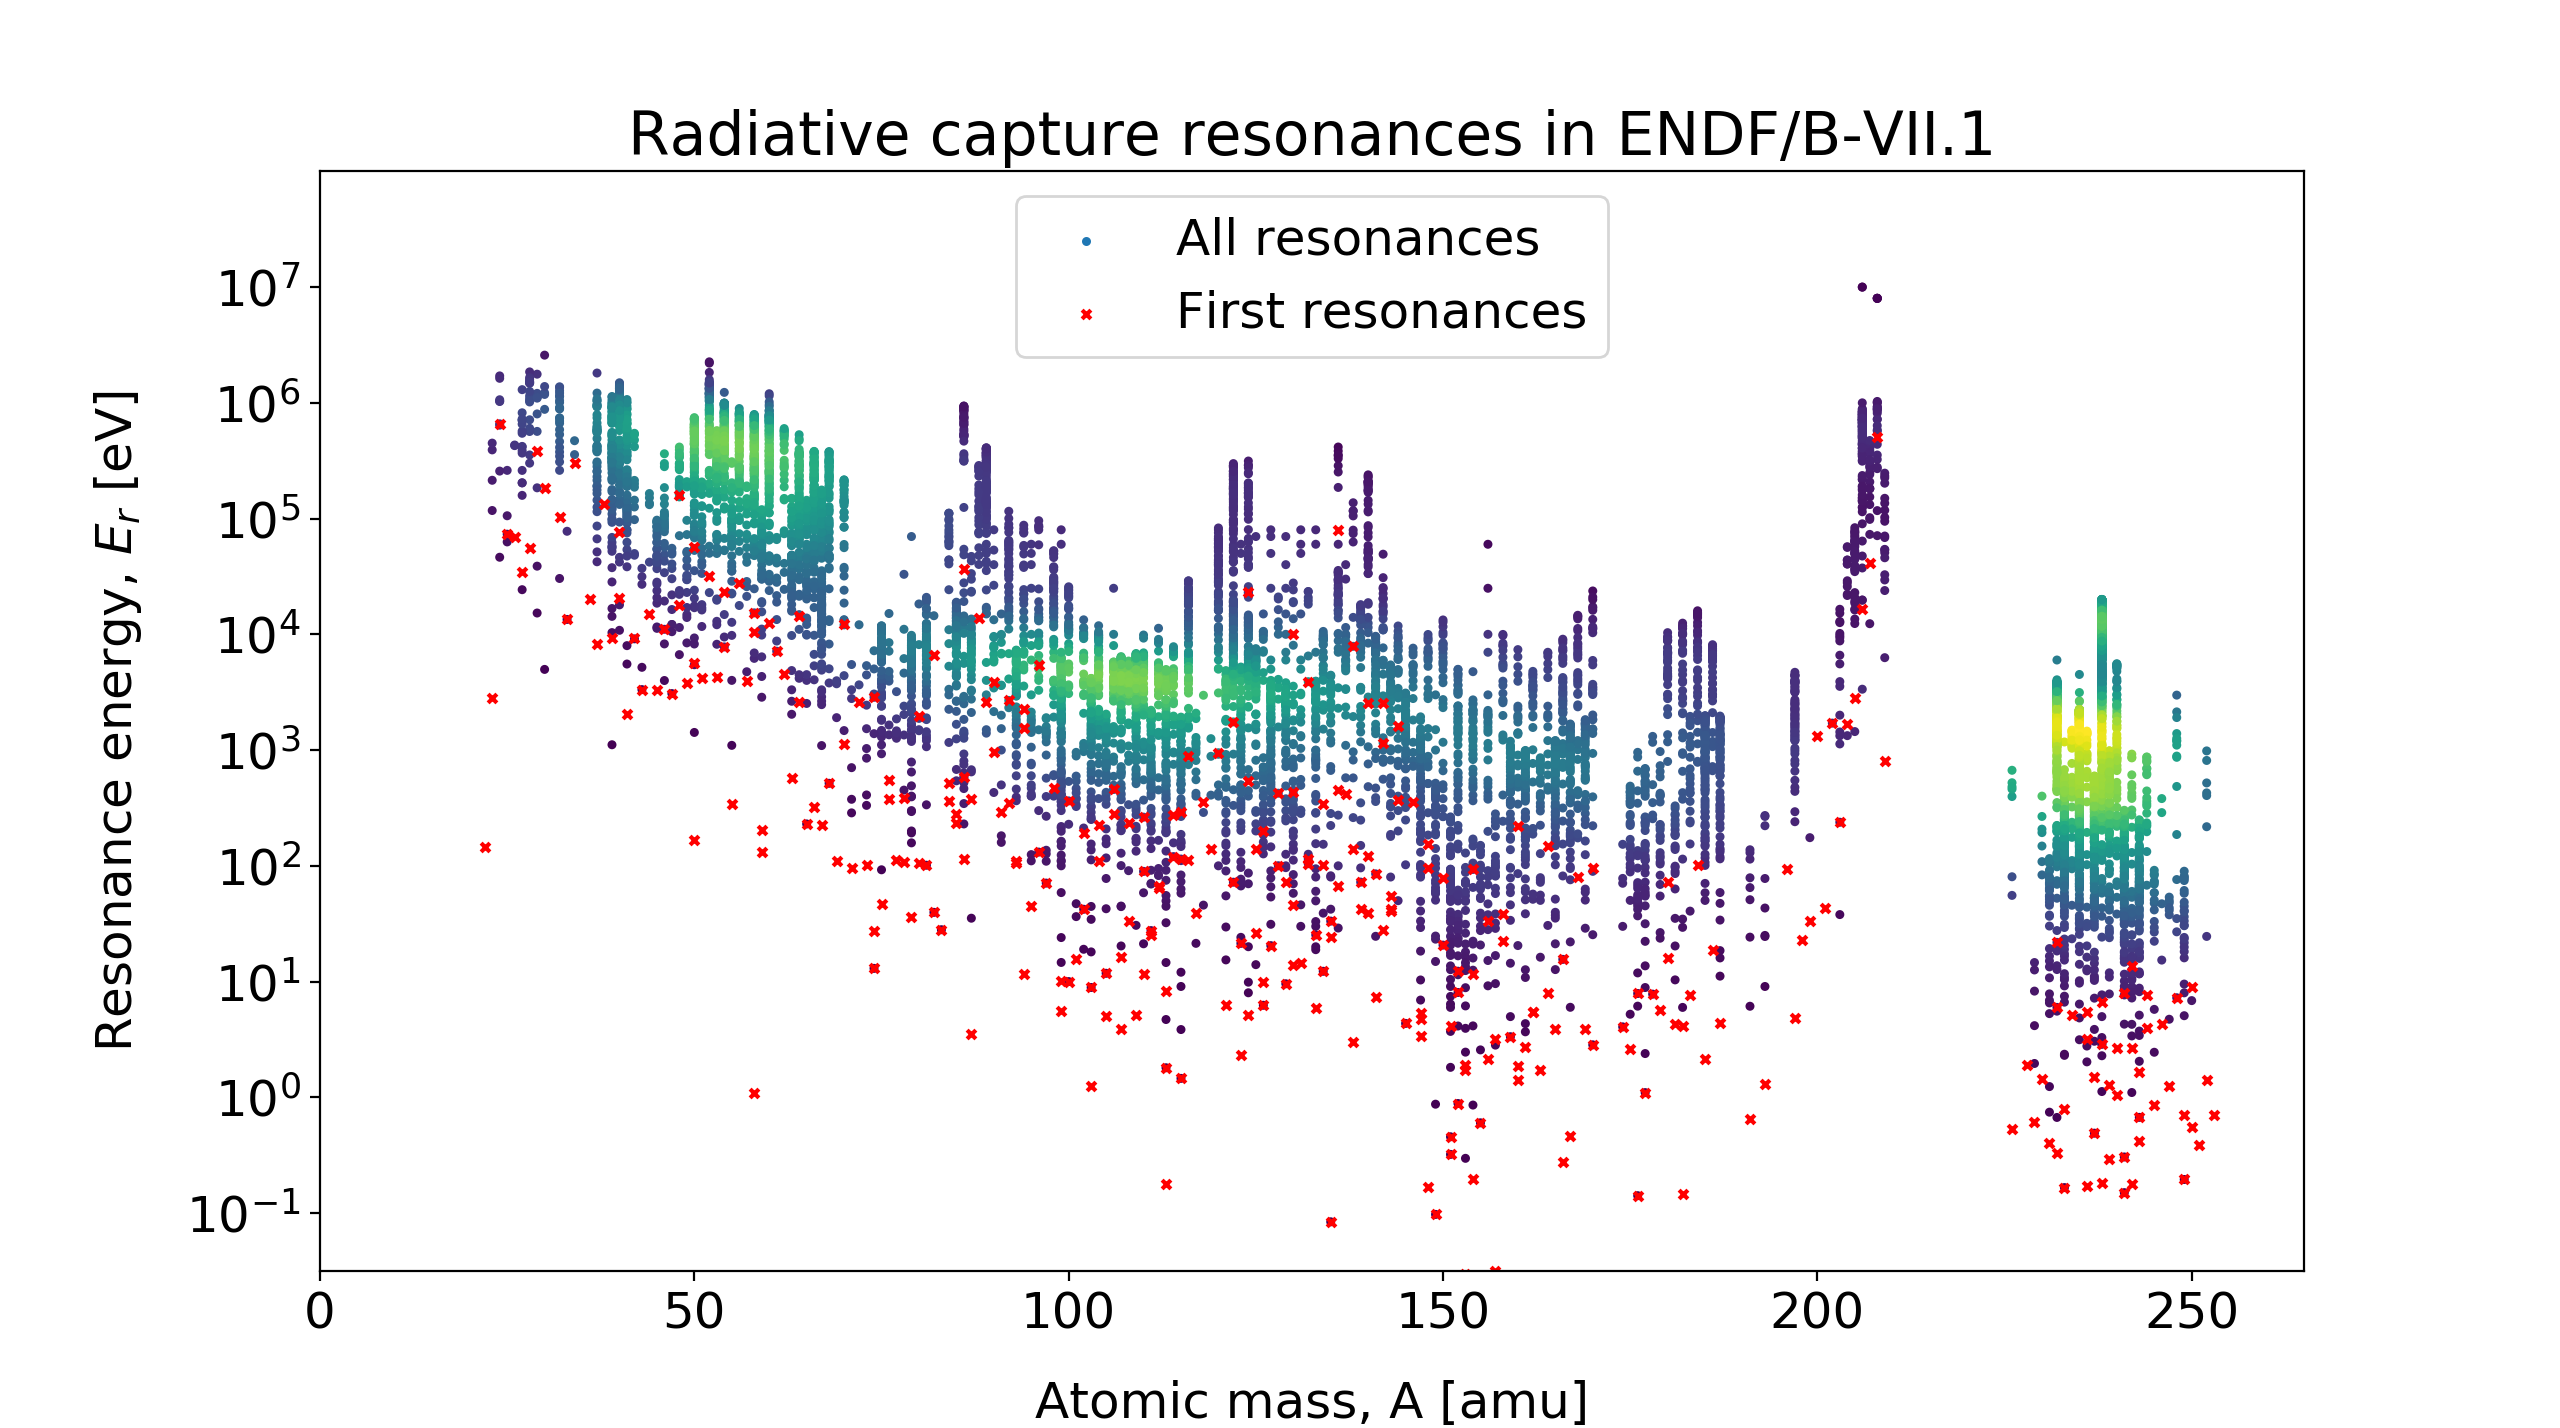
\includegraphics[width=\linewidth]{resonance_energy_atomic_mass}
  \caption{This scatter plot shows the energy of resonances as a function of atomic mass, for the majority of resonances recorded in the ENDF/B-VII.1 nuclear data library. The data are coloured by density, with blue as lowest density, green medium and yellow highest. The density has been calculated in \{log\textsubscript{10}(E), A\} space with a Kernel Density Estimator (KDE) approach. The first resonance for each nuclide is marked by a red cross for ease of identification.}
  \label{fig:res_energy_mass}
\end{figure}

Figure~\ref{fig:res_energy_mass} shows the general trend for lower energy resonances with increasing atomic mass. This trend is most pronounced up to $\mathrm{A} \approx 150$. After this point, the relationship flattens off for very large mass nuclides ($\mathrm{A} > 220$) and is completely invalidated for nuclides with $\mathrm{A} \approx 210$, the region of Pb \& Bi. Nuclides in this range are especially stable, close to the `magic numbers' of stable nuclei predicted by the nuclear shell model \cite{Stone1997}. Here, nucleons are especially tightly bound and a large energy input is required to reconfigure the nucleus. The highest density region is that of the actinides, where each nucleus has very many nuclear resonances, at comparatively low energies. Looking more generally, it can be seen that resonances are typically present for perhaps as much as 5 orders of magnitude of the energy spectrum for a given mass, a very large window. Taking all nuclides into account, resonances appear within the $10^{-1} < E_{r}\mathrm{[eV]} < 10^{7}$ range. If we assume that all resonances are equally important to consider when designing a group structure, then a fine grid might be required across this entire range, from practically thermal neutrons to unmoderated DT neutrons. 

\nomenclature[z]{KDE}{Kernel Density Estimator}
\nomenclature[z]{RI}{Resonance Integral}

% Need to introduce the concept of a resonance integral, refer back to BW description and describe our integration
We can quantify the `size' of a particular resonance by integrating a relevant descriptive function across some characteristic energy range, this so-called Resonance Integral (RI) is specified by equation~\ref{eq:res_integral}. 

\begin{equation}
  \label{eq:res_integral}
  RI = \int_{E_{r}-4\Gamma}^{E_{r}+4\Gamma} \frac{\pi\lambdabar^{2}(2J + 1)}{(2s_{n} + 1)(2s_{t} + 1)}  \frac{\Gamma_{i}\Gamma_{f}}{[(E-E_{r})^{2} + \Gamma^{2}_{t}/4]} dE
\end{equation}
% Very useful reference: http://www-pnp.physics.ox.ac.uk/~barra/teaching/resonances.pdf

Where $E$ is centre-of-mass energy of the system, $\Gamma_{i}$ is the partial resonance width to decay to the initial state, $\Gamma_{f}$ is the partial width to decay to the final state, $\Gamma_{t}$ is the total width, $\lambdabar$ the reduced particle wavelength, $E_{r}$ the rest mass energy of the resonance, $J$ the total angular momentum of the resonance, $s_{n}$ the neutron spin and $s_{t}$ the target spin \cite{Libby2005}. For formation of a compound nucleus by an incident neutron, leading to subsequent neutron emission, $\Gamma_{i}$ = $\Gamma_{f}$ = $\Gamma_{n}$, giving $\Gamma^{2}_{n}$ in the numerator. For radiative capture, it is instead $\Gamma_{n}\Gamma_{\gamma}$. 

RIs give an indication of the resonance's contribution to reaction rate. Computing the RI for all the resonances parsed in ENDF/B-VII.1 we can identify the largest and thus the most important to correctly represent in any energy discretisation scheme. These largest resonances are plotted as a function of energy in figure~\ref{fig:largest_res_energy_scatter}. Given these data are a subset of those presented in figure~\ref{fig:res_energy_mass}, many of the same trends as visible, such as the inverse relationship between energy and atomic mass. These largest resonance data do tend to be at the lower energy of the complete set and indeed further analysis shows that 20\% of the lowest energy neutron scattering resonances are also those with the largest RI for that nuclide. For radiative capture resonances, this figure is 41\%\footnote{The difference is because neutron scattering partial widths are correlated with interaction energy, whereas partial gamma widths are roughly constant (see figure~\ref{fig:res_correlation}).}. As such, it is not the case that the lowest energy resonances for each nuclide have always or even more often the largest RI. Any energy group structure optimisation routine should not simply target these resonances.

\begin{figure}[H]
  \centering
  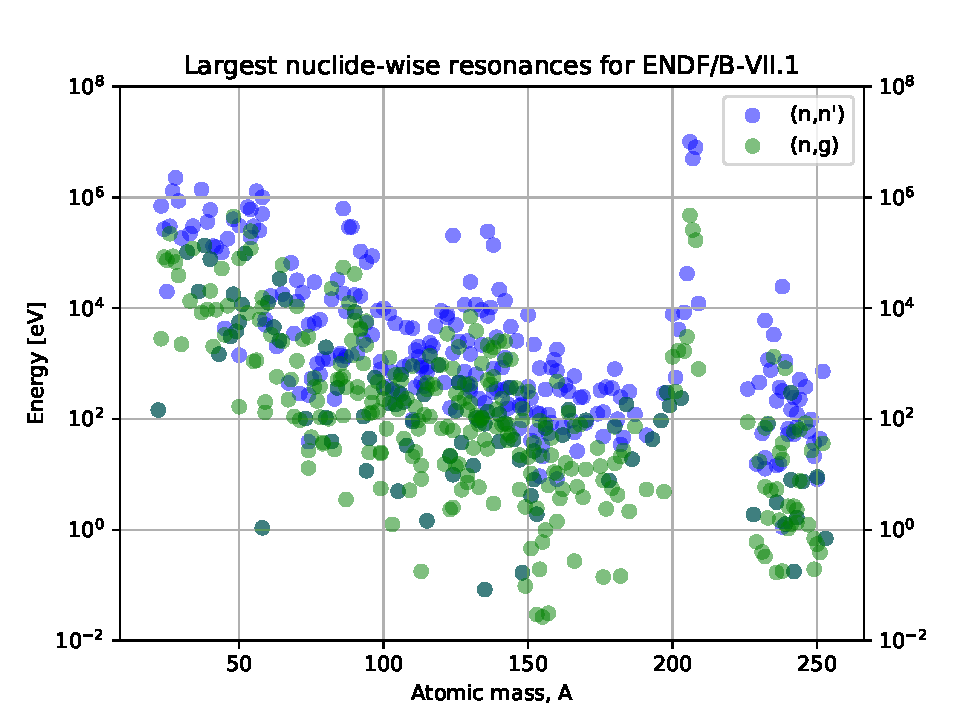
\includegraphics[width=\linewidth]{largest_res_energy_scatter}
  \caption{The energy of the largest resonances for ENDF/V-BII.1 as a function of atomic mass. The `largest' is determined by the RI as defined in equation~\ref{eq:res_integral}. Two datasets are shown, RI calculated using widths for neutron emission, $\Gamma_{n}$ in blue and for gamma emission, $\Gamma_{\gamma}$ in green.}
  \label{fig:largest_res_energy_scatter}
\end{figure}

It is instructive to inspect the correlations between various parameters recorded in the assembled resonance database. A correlation matrix of selected parameters is shown as figure~\ref{fig:res_correlation}. As previously shown in figure~\ref{fig:res_energy_mass} resonance energy and atomic mass are inversely correlated. $\Gamma_{n}$ is correlated with energy, while $\Gamma_{\gamma}$ is not. Given $\Gamma_{t} = \Gamma_{n} + \Gamma_{\gamma} + \Gamma_{f}$ but $\Gamma_{\gamma}$ is largely constant and $\Gamma_{f}$ is only important for a few resonances in particular nuclides, $\Gamma_{t}$ displays largely the same relations as $\Gamma_{n}$. 

\begin{figure}[H]
  \centering
  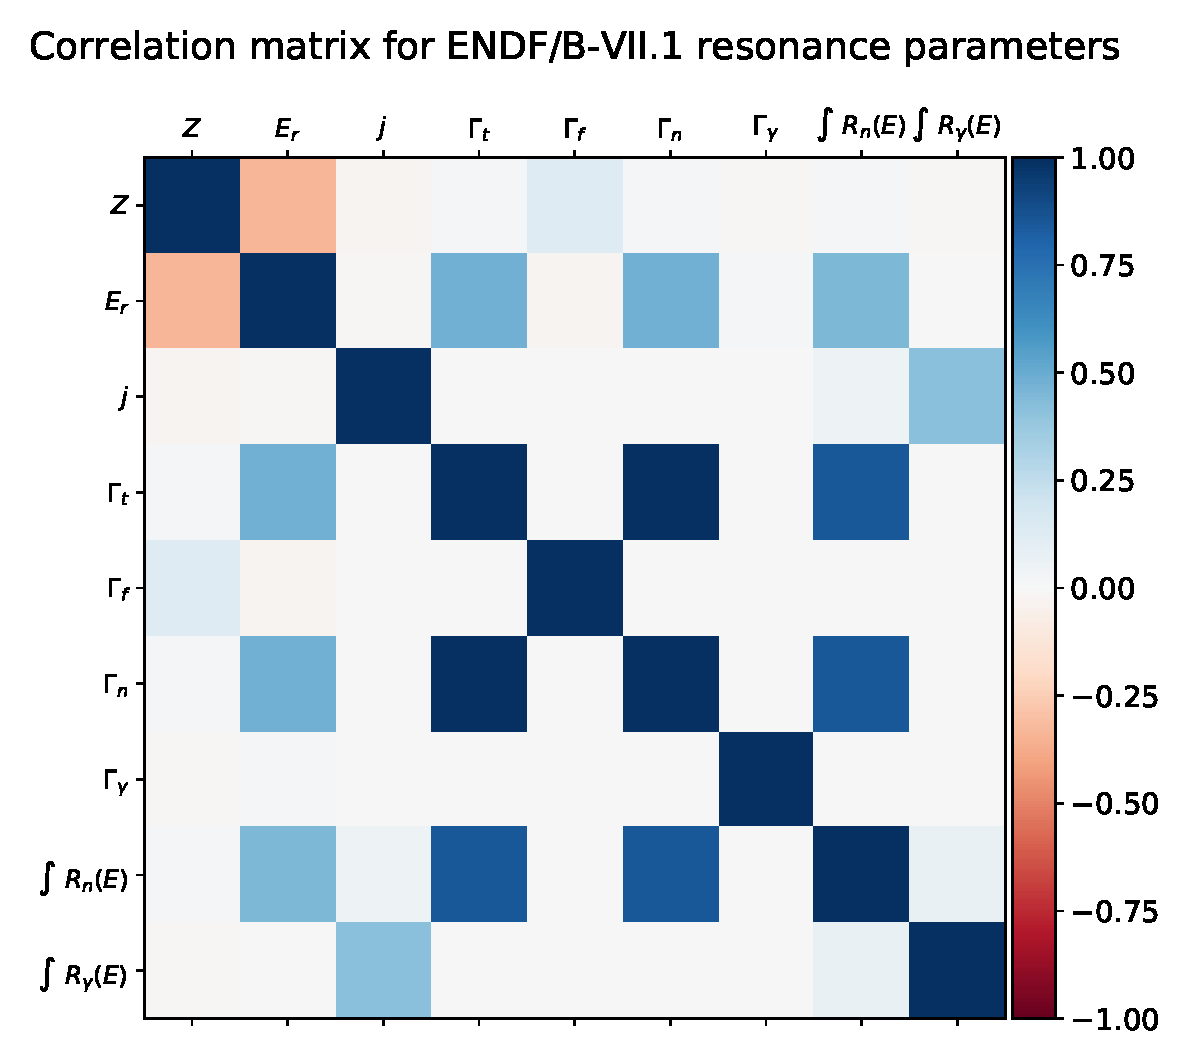
\includegraphics[width=\linewidth]{res_correlation}
  \caption{This correlation matrix is assembled from the resonance parameter data contained within the ENDF/B-VII.1 nuclear data library. It is constructed from the covariance matrix, showing how pairs of variables vary together, but normalised such that a meaningful comparison between relationships can be undertaken. The normalisation is given here \cite{numpy2018}. $A$ is atomic mass, $E_{r}$ resonance centre-of-mass energy, $l$ neutron orbital angular momentum, $J$ the total angular momentum, $\Gamma_{t}$ the total width, $\Gamma_{f}$ the fission partial width, $\Gamma_{n}$ the neutron emission partial width, $\Gamma_{\gamma}$ the $\gamma$-ray emission partial width, $\int R_{n}(E)$ the resonance integral for $\Gamma_{n}$ and $\int R_{\gamma}(E)$ the resonance integral for $\Gamma_{\gamma}$.}
  \label{fig:res_correlation}
\end{figure}

% So if we can determine which resonances are `biggest', how they are those ones inparticular distributed?
% Which features are there? 
% What causes them?
% Is any of this information useful to us?

% \begin{figure}[H]
%   \centering
%   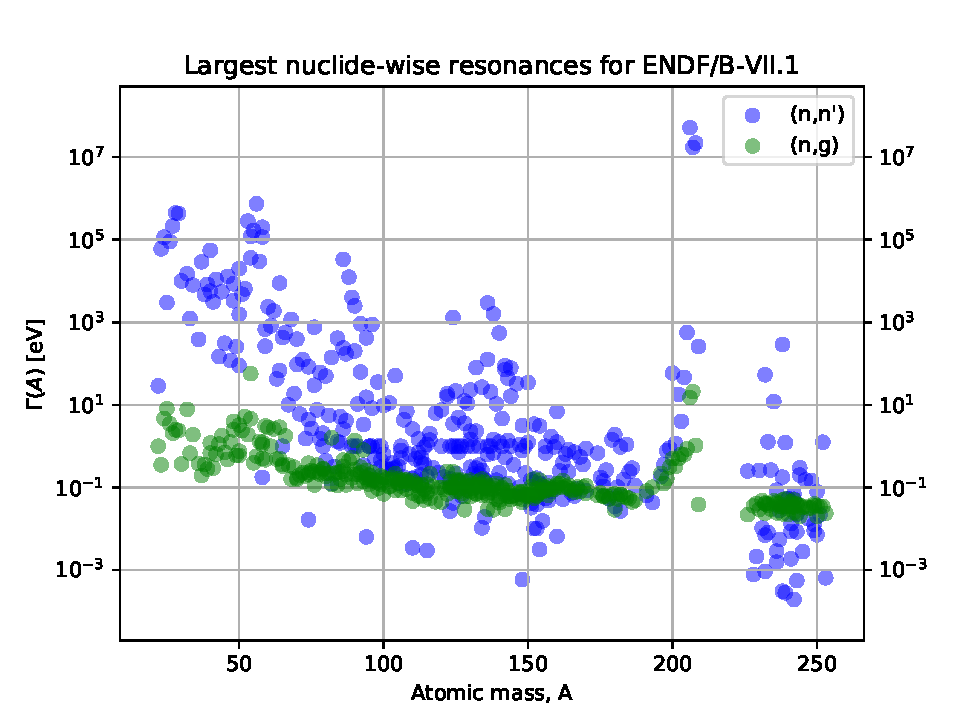
\includegraphics[width=\linewidth]{largest_res_width_scatter}
%   \caption{}
%   \label{fig:}
% \end{figure}

\subsection{Self-shielding}
\label{subsec:self-shielding}
The phenomenon of self-shielding is that whereby a particle flux is depleted in certain energy regions through absorption by the containing medium. This then `shields' the rest of the medium from those particle energies and decreases reaction rates. If this reduction in flux is not fed back then reaction rates will be overestimated. This effect is a particular problem where cross-sections and spectra are discretised into group-wise formats, as in deterministic radiation transport and activation-transmutation calculations. If energy groups are too large, flux depressions cannot be resolved.

Introducing \citeauthor{Bondarenko1964}'s self-shielding method exemplifies why a self-shielding treatment is necessary, how one can work and why it might be of interest for optimising group structures. 

Here we define an energy group, $E = [E_{0}, E_{1}, \dots, E_{G}]$ with $G$ groups. The lowest energy is $E_{0}$ and the highest $E_{G}$. The groups are in ascending energy order, so $E_{g+1} > E_{g}$, with the width of group $g$ given as $\Delta E = E_{g+1} - E_{g}$. To determine reaction rates, i.e. $RR(E) = N\sigma(E)\phi(E)$, where $N$ is the atomic density of the material, $\sigma(E)$ the cross-section and $\phi(E)$ the flux we need both the cross-section and the flux as a function of energy.

The flux for some group, $\phi_{g}$ is given by equation~\ref{eq:group_flux}.

\begin{equation}
  \label{eq:group_flux}
  \phi_{g} = \int_{E_{g}}^{E_{g+1}} \phi(E) dE
\end{equation}

We can define the group cross-section as equation~\ref{eq:group_cross_section}.

\begin{equation}
  \label{eq:group_cross_section}
  \sigma_{g} = \frac{\int_{E_{g}}^{E_{g+1}} \sigma(E) \phi(E) dE}{\int_{E_{g}}^{E_{g+1}} \phi(E) dE}
\end{equation}

$\sigma_{g}$ must be defined in such a way that it accurately reproduces the RR when multiplied by the flux. Unfortunately, equations~\ref{eq:group_flux} and \ref{eq:group_cross_section} require knowledge of $\phi(E)$ within a group, the quantity sought. If $\phi(E)$ were constant, then equation~\ref{eq:group_cross_section} would reduce to $\sigma_{g} = \int_{g}^{g+1} \sigma(E) dE$. While this is sometimes a reasonable assumption, if resonances are present in the group it is not. 

Looking for an expression to substitute for $\phi(E)$ we could first examine the total cross section of the system. Assuming a homogeneous mixture of M nuclides the total macroscopic cross section, $\Sigma_{t}$ is given by equation~\ref{eq:macroscopic_xs} where $N^{m}$ is the number density of nuclide $m$

\begin{equation}
  \label{eq:macroscopic_xs}
  \Sigma_{t}(E) = \sum_{m}^{M} N^{m} \sigma_{t}^{m}(E)
\end{equation}

The product of the energy varying flux, $\phi(E)$ and total macroscopic cross-section, $\Sigma_{t}(E)$ is the `collision density', $\phi(E) \Sigma_{t}(E) = S(E)$, or expressed equivalently as equation~\ref{eq:collision_density}.

\begin{equation}
  \label{eq:collision_density}
  \phi(E) = \frac{S(E)}{\Sigma_{t}(E)}
\end{equation}

If we let $S(E)$ be some smooth function, say a Maxwell-Boltzmann distribution or a 1/E particle slowing down spectrum, equation~\ref{eq:collision_density} shows us how the total cross-section impinges on the flux. A resonance within $\Sigma_{t}(E)$ causes $\phi(E)$ to drop, a flux depression. Substituting equation~\ref{eq:collision_density} into equation~\ref{eq:group_cross_section} gives the following:

\begin{equation}
  \label{eq:group_xs_s}
  \sigma_{g}^{m} = \frac{\int_{E_{g}}^{E_{g+1}} \sigma(E)^{m} \frac{S(E)}{\Sigma_{t}(E)} dE}{\int_{E_{g}}^{E_{g+1}} \frac{S(E)}{\Sigma_{t}(E)} dE}
\end{equation}

Equation~\ref{eq:group_xs_s} gives $\sigma_{g}^{m}$, the group cross-section for nuclide $m$, and can be used to generate all group cross-sections of interest for the problem if an appropriate $S(E)$ can be assumed. The macroscopic cross-sections on the right hand side of equation~\ref{eq:group_xs_s} are both total cross sections as any interaction will lower the flux. In the limiting case where the energy group width narrows to 0, $S(E)$ becomes constant, i.e. $\lim_{\Delta E \to 0} S(E) = k$ and $S(E)$ cancels from equation~\ref{eq:group_xs_s}. When energy group structures have a high bin density, they are reducing their reliance on this $S(E)$ function assumption.

The background cross-section is a concept introduced by \citeauthor{Bondarenko1964}. Cross-sections may belong to two mutually exclusive categories, they are either the cross-section of interest, or belong to a set `background' cross-sections which, if of sufficient magnitude act to depress the particle flux and shield the cross-section of interest. The macroscopic cross-section, $\Sigma_{t}(E)$ of equation~\ref{eq:macroscopic_xs} is then written as in equation~\ref{eq:background_xs}.

\begin{equation}
  \label{eq:background_xs}
  \Sigma_{t}(E) = N^{m} \sigma_{t}^{m}(E) + \sum_{n \neq m}^{M} N^{n} \sigma_{t}^{n}(E)
\end{equation}

We can factor out the number density for our nuclide of interest, $m$, to give equation~\ref{eq:background_factored}. 

\begin{equation}
  \label{eq:background_factored}
  \Sigma_{t}(E) = N^{m} (\sigma_{t}^{m}(E) + \sigma_{0}^{m}(E))
\end{equation}

Here $\sigma_{0}^{m}(E)$ is not a cross-section of nuclide $m$ in the normal sense, but all the cross-sections that contribute to its `background'. It is defined as equation~\ref{eq:background_xs_def}.

\begin{equation}
  \label{eq:background_xs_def}
  \sigma_{0}^{m}(E) = \frac{1}{N^{m}} \sum_{n \neq m}^{M} N^{n} \sigma_{t}^{n}(E)
\end{equation}

We can combine equations~\ref{eq:group_xs_s}, \ref{eq:background_factored} and \ref{eq:background_xs_def} to give equation~\ref{eq:group_xs_background}, where energy dependence is omitted for readability.

\begin{equation}
  \label{eq:group_xs_background}
  %\sigma_{g}^{m} = \frac{\int_{E_{g}}^{E_{g+1}} \sigma^{m}(E) \frac{S(E)}{\sigma_{t}^{m}(E) + \sigma_{0}^{m}(E)} dE}{\int_{E_{g}}^{E_{g+1}} \frac{S(E)}{\sigma_{t}^{m}(E) + \sigma_{0}^{m}(E)} dE}
  \sigma_{g}^{m} = \frac{\int_{E_{g}}^{E_{g+1}} \sigma^{m} \frac{S}{\sigma_{t}^{m} + \sigma_{0}^{m}} dE}{\int_{E_{g}}^{E_{g+1}} \frac{S}{\sigma_{t}^{m} + \sigma_{0}^{m}} dE}
\end{equation}

The group cross-section for a given nuclide, $\sigma_{g}^{m}$, is a function of the background cross-section. Further detail on the above derivations are available in \cite{Dembia2013} \cite{Bell1970}. 

If the background cross-section and the point-wise cross-section to be grouped are known, one can compute the $\sigma_{g}^{m}$, the shielded cross-section and go on to accurately compute reaction rates and other responses of interest. It is convenient to define a number which is the ratio of the unshielded and shielded cross-sections. This `self-shielding factor', or SSF, is of the range [0,1] where 1 indicates there is no self-shielding occuring, so any reaction rates are the simple multiplication of particle flux and unmodified cross-section. For values closer to 0, the cross-section is revised down, reducing the reaction rate. 

Figure~\ref{fig:W-183_shielding} shows cross-sections from several tungsten istopes, \textsuperscript{182}W, \textsuperscript{183}W, \textsuperscript{184}W and \textsuperscript{186}W which together account for 99.88\% of the atomic mass of natural W. When computing the self-shielding factors for \textsuperscript{183}W in a material of natural W, it can be seen that areas without a significant background cross-section such as $140 < E [eV] < 160$, the self-shielding factors make a greater change to the unshielded cross-section. However, some resonances from different isotopes overlap in energy. Where there is a large resonance from an isotope other than nuclide in question, it elevates the background cross-section, $\sigma_{0}$, and absorbs particles in this energy region. An example of this behaviour is the \textsuperscript{183}W resonance at 220 eV, which is overshadowed by resonances in \textsuperscript{182,186}W and so does not significantly self-shield. The self-shielding factor for this energy bin is correspondingly close to unity.

% Plot of self-shielding factor with background cross-sections, showing shielding on lone target resonance, less shielding with high background
\begin{figure}[H]
  \centering
  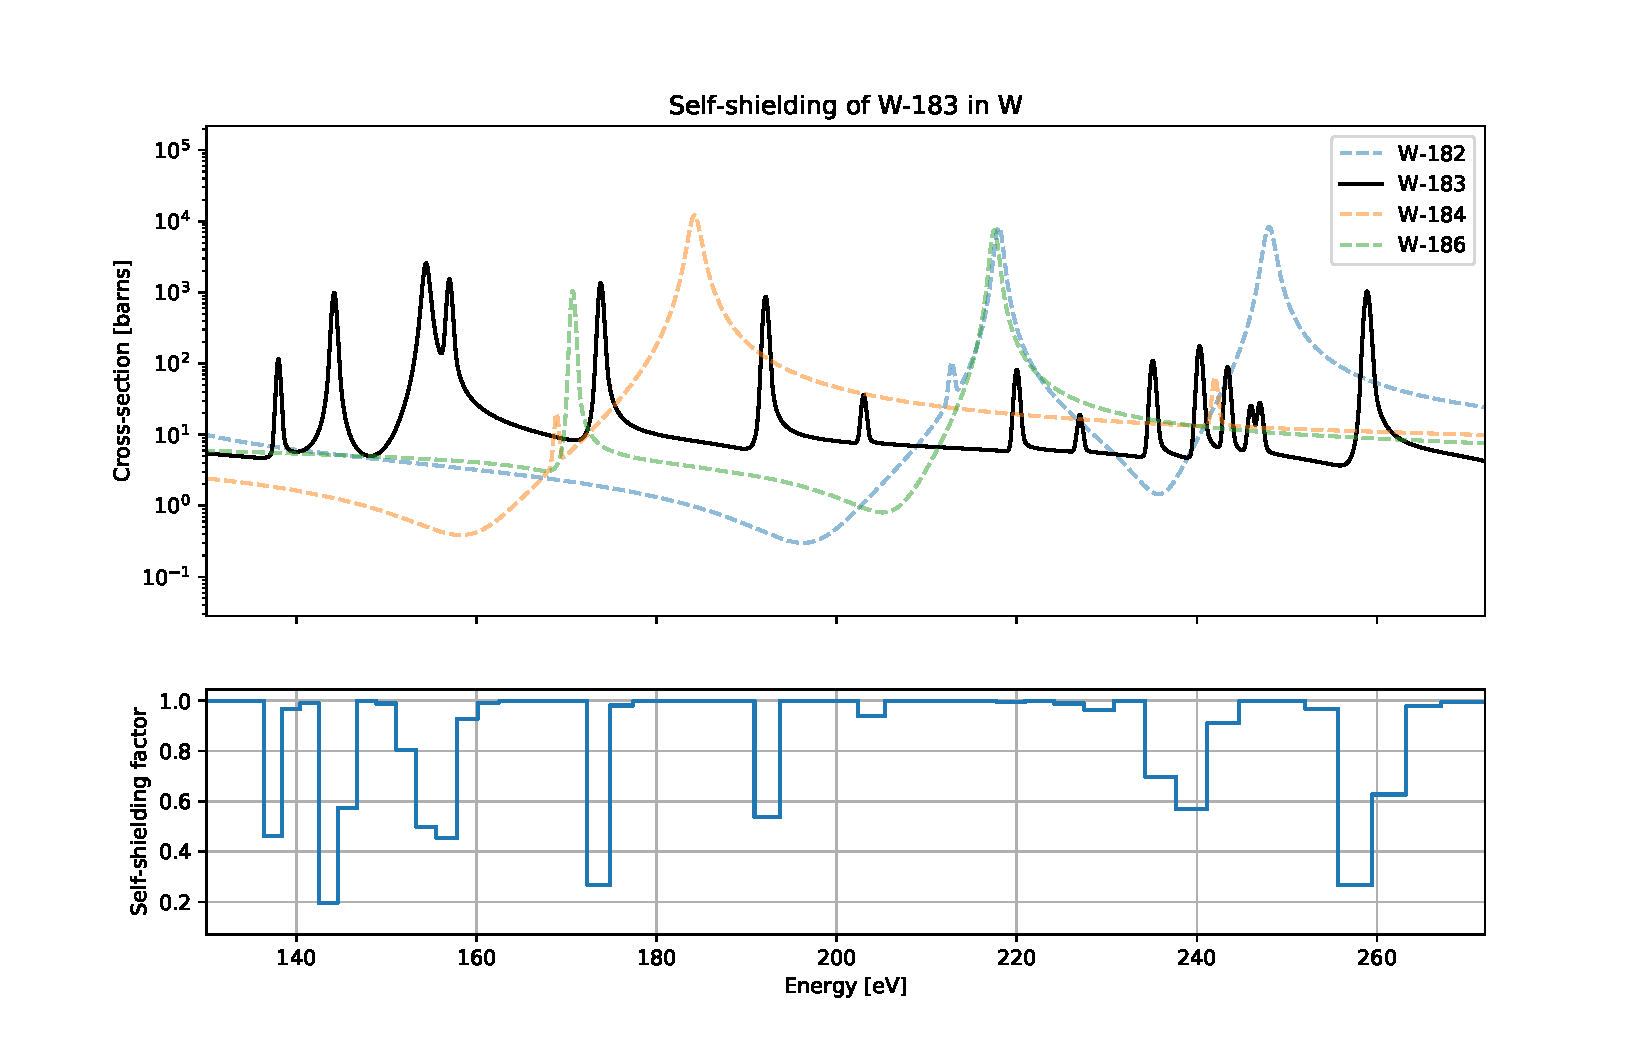
\includegraphics[width=\linewidth]{W-183_shielding}
  \caption{This figure shows cross-sections and computed self-shielding factors for \textsuperscript{183}W in elemental tungsten. The upper panel shows the total cross-section, $\sigma_{t}(E)$, for the major constituent isotopes of tungsten. The interaction data is processed from ENDF-B/VII.1 and was obtained from \citeauthor{Shimwell2018}'s online cross-section plotting service \cite{Shimwell2018}. The lower panel shows total self-shielding factors computed for group-wise \textsuperscript{183}W data using the FISPACT-II code \cite{sublet2017a}. The group structure employed is a relatively fine 2,048 group with equal log\textsubscript{10} spacing. Note how \textsuperscript{183}W resonances are only shielded when the have a greater cross-section than other nuclides in the mixture (natural tungsten).}
  \label{fig:W-183_shielding}
\end{figure}

Calculating self-shielding factors by the above method, or other more sophisticated approaches, allows one to then take simple unshielded cross-sections, multiply then by the SSF and arrive at group cross-sections that are more appropriate for the nuclide given its environment. A convenient measure of the magnitude of this shielding is given by equation~\ref{eq:ssf_bar}.

\begin{equation}
  \label{eq:ssf_bar}
  \overline{\mathrm{SSF}} = \frac{\sum_{g=0}^{G}\mathrm{RR}(E_{g})\mathrm{SSF}(E_{g})}
                                          {\sum_{g=0}^{G}\mathrm{RR}(E_{g})}
\end{equation}

An example application of group-wise self-shielding factors is shown in figure~\ref{fig:W183_gamma}. Here self-shielding factors have been applied to a na\"ive, unshielded group-wise (n,$\gamma$) reaction-rate, reducing the total energy-integrated reaction rate to 0.364 of its unshielded value. Note the log-scale of the ordinate axis--the groups in the immediate vicinty of the three resonances contribute much of the total reaction rate and significant shielding on one of these groups can severely change the result.

% Perhaps a simple plot of self-shielding factor, unshielded and shielded RR in ssf_data/709_fispact/figures
\begin{figure}[H]
  \centering
  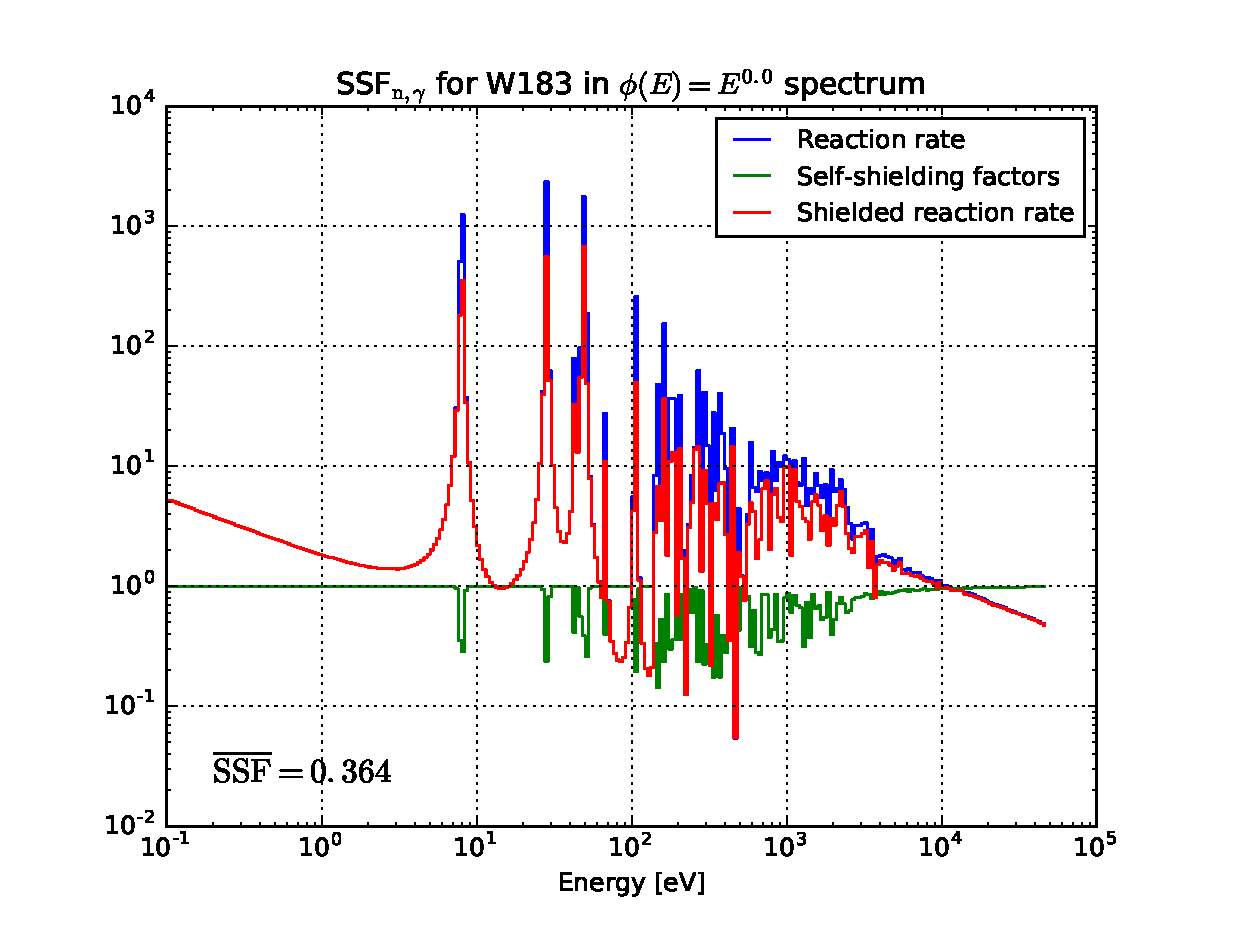
\includegraphics[width=\linewidth]{W183_gamma}
  \caption{Shown here are the unshielded and shielded \textsuperscript{183}W(n,$\gamma$)\textsuperscript{184}W reaction rates and the associated macro-partial self-shielding factors for this reaction channel as a function of energy. The neutron spectrum in this example is a constant function of energy and so the reaction rates are a simple renormalisation of the cross-section. The material is elemental tungsten.}
  \label{fig:W183_gamma}
\end{figure}

The calculation of reaction rates should incorporate the effects of self-shielding. As indicated above, a resonant material of particular interest to fusion plant designers is tungsten. Figure~\ref{fig:W183_gamma} highlights the difficulties of determining reaction rates to a high accuracy. $^{183}$W has a large resonance at 8 eV and the energy-integrated reaction rate within this and neighbouring resonances typically dominate the total reaction rate. With the coarse group structure shown in the figure, an unshielded approach to computing the reaction rate yields values several times the `true' point-wise value. \citeauthor{Pampin2005} showed the importance of self-shielding for tungsten in fusion applications, finding that neglecting shielding effects can overestimate radiative capture in \textsuperscript{186}W by a factor of 6. \citeauthor{Gilbert2016}'s work built on this, sampling flux at multiple depths in first-wall tungsten to predict accurate rates of transmutation to rhenium and osmium. Even with this more sophisticated modelling approach, total unshielded reaction rates were sometimes twice their true value \cite{Gilbert2016}. The self-shielding of resonant materials other than tungsten has yet to receive much attention in nuclear analyses of fusion power systems. Examples from the fission realm also abound, using a relatively coarse (but commonplace) 175 group structure \cite{Plechaty1978}, individual groups for \textsuperscript{232}Th cross-sections can be wrong by a factor of 50 \cite{Cacuci2010}. 

Various methods exist for computing the effects of self-shielding, including the one laid out above. These methods have been validated in a variety of scenarios, especially with regards to the fission realm. However, the deployment of these methods to geometrically complex heterogeneous systems such as a fusion reactors is not a straightforward prospect. Undoubtedly self-shielding effects must be included in future studies, but reliance upon the computation of accurate self-shielding factors should be reduced where possible. Assume SSF(E\textsubscript{g}) is a self-shielding factor, where g is some group containing a large, self-shielded resonance--if $\mathrm{SSF(E_{g})} \approx 0.1$, a mere 0.01 error in this one factor results in a 10\% error for the group cross-section and may dramatically change the total reaction rate. 

To reduce the requirement for the accurate computation of self-shielding factors, one can adopt a higher-fidelity description of interaction and particle spectrum data. However, as seen earlier, many tens of thousands of groups are required for the accurate computation of reaction rates when used in an untargeted way. The remainder of this chapter uses concepts from self-shielding to \textit{target} bin density resolution for optimised energy group structures. 

% Curse shielding, as in something to be minimised, but self-shielding theory and associated SSFs an opportunity for attacking the problem

%The rest of this paper details the first results of one approach, namely the intelligent discretisation of spectra and nuclear data to narrow important groups and make S(E) constant with E. Any remaining errors taken account of with self-shielding factors.

%\subsection{JET}

\section{Method}
\label{sec:method}
The general approach adopted here for optimising energy group structures is to use functions derived from group-wise cross-section and self-shielding data to construct a distribution that represents how badly represented each part of the energy domain is for a given set of reactions. After modifications, this distribution is used as a bin density distribution, allowing a given number of bins to be apportioned by need throughout the energy domain. 

This approach requires a robust, repeatable methodology for the generation of nuclear data on an arbitrary energy grid. Section~\ref{subsec:nd_processing} outlines this. Then, section \ref{subsec:opt} describes how a bin density distribution can be derived from self-shielding data. Finally, section \ref{subsec:computation} details the computational methods utilised to test the optimised group structures.

\subsection{Nuclear data processing}
\label{subsec:nd_processing}
As mentioned in chapter~\ref{chap:tmc} with regard to the TENDL nuclear data libraries, a key to producing reliable nuclear data is having a processing architecture that is robust and repeatable \cite{Koning2008}. For this group structure optimisation work, many kinds of nuclear data are required. The production of this data was coordinated by a series of Python modules and scripts written during the project. These launched other codes, parsing and checking outputs before inputting these to other codes. Below is a short description of the attributes and production process for each kind of relevant nuclear data.
% Describe infrastructure: design, robustness, testing, types of data
% Some sort of flowchart?

\subsubsection{Group structure}
The group structure is defined by an ebins file, as per FISPACT-II. These stipulate the position of energy bounds, at 7 digit precision with 2 digits for the order of magnitude\footnote{See \cite{Cullen1988} for effects of ND numerical precision on calculations.}. The file is in descending order energy, with units of electron-volts. The ebins file is given a unique ID that is also used for all grouped data which adopt its group structure.

\subsubsection{Evaluated Nuclear Data Files (ENDF)}
The ENDF files used for this work were those of the ENDF/B-VII.1 library \cite{Chadwick2011}.

\subsubsection{Point-wise ENDF (PENDF)}
Point-wise, or PENDF files are created using NJOY \cite{MacFarlane2016}. Resonances were constructed with the reconr module. For all work presented here the resonances were Doppler broadened to room temperature (294K) with the broadr module. 

\subsubsection{Group-wise ENDF (GENDF)}
Group-wise data, or GENDF files were produced from the broadened PENDFs using the groupie module of the PREPRO processing code \cite{cullen2017}. This operation takes a group structure specified by an ebins description.

\subsubsection{Probability tables}
To enable self-shielding calculations within the unresolved resonance range, probability tables were employed (see section~\ref{subsec:prob_table} in chapter~\ref{chap:introduction}). These were computed with the CALENDF code \cite{sublet2011}. This is the most computationally expensive step of the ND generation and was parallelised to utilise multiple cores with the Python multiprocessing module \cite{multiprocessing2018}.

\subsubsection{Self-shielding factors}
The computation of self-shielding factors was accomplished with FISPACT II, version 3.2 \cite{sublet2017a}. Inputs include the group structure, ENDF file, group-wise interaction data, probability tables, nuclides to shield, containing material, material temperature and incident particle spectrum. Each calculation would compute the self-shielding factors for all available macro-partial cross-sections (neutron scattering, radiative capture, fission) and the total. 

The target nuclide would be defined within its elemental material, i.e. \textsuperscript{56}Fe would be shielded for a \textsuperscript{nat.}Fe mixture. Clearly, many times nuclides are present within materials of more than their element, whenever they are compounded or alloyed. However, it can be almost guaranteed that nuclides are present alongside fellow isotopes. Given that the aim of this study is to use self-shielding factors to target bin resolution rather than accurately calculating a specific reaction rate or rates, this `elemental composition' assumption was deemed acceptable as providing likely background cross-sections for the shielding calculation. 

FISPACT can take an arbitrary particle spectrum as input. For the simulations described below two broad cases were used: 

\begin{enumerate}
  \item Realistic spectra, sampled from a stochastic radiation transport code (MCNP6). These were sampled in the relevant group structure and allow comparison between group-wise and point-wise calculations. 
  \item `Parametric spectra' where a flux for each group structure bin was calculated from a relationship of the sort: $\log_{10}\phi(E) = m\log_{10}(E) + c$, a linear relationship in log-log space. If $c = 0$, this is simply $\phi(E) = E^{m}$. By varying $m$, the gradient of the slowing-down region can be modified and greater weight given to cross-sections (and resonances) within the low or high energy regions. This $m$ parameter is an input to the optimisation process outlined below, in section~\ref{subsec:opt}.
\end{enumerate}

\subsubsection{A Compact ENDF (ACE)}
To enable testing of optimised group structures, point-wise calculations using MCNP6 are used as a reference. The underlying nuclear data used in this simulation should be the same as that used to create the discretised data. As such, ACE files for MCNP6 are produced from the ENDF/B-VII.1 data at 294K, using the acer module of NJOY \cite{MacFarlane2016}.

\subsection{Group structure optimisation}
\label{subsec:opt}
Accurate nuclear simulations require cross-section data which preserve the true reaction rates even when discretised. An energy-dependent function of the reaction rate accuracy could be used to indicate where a higher-fidelity representation of the resonance would be useful. If this action could be performed for a variety of cases (materials, common spectra), this function could be used to target group structure bin density, lessening future errors. The process could perhaps be performed iteratively to converge on an ideal group structure. The group structure could be very specific (for a certain reaction channel and spectrum) or relatively general (for the whole table of nuclides, in a typical slowing down spectrum).

\subsubsection{Towards an ideal bin density function}
To assemble a distribution for bin density we define several piecewise functions for identifying where, in the energy domain, self-shielding factor modifications are important and to indicate where resolution should be concentrated. 

Equation~\ref{eq:s} describes the cumulative differences between reaction rates for an energy group as defined in section~\ref{subsec:self-shielding}. 

\begin{equation}
  \label{eq:s}
  S(E_{g}) = \sum_{i=0}^{g} (\mathrm{RR}(E_{i}) - \mathrm{RR}(E_{i})\mathrm{SSF}(E_{i}))
\end{equation}

$S(E_{g})$ is the sum of differences between shielded and unshielded reaction rates from the start of the resolved resonance region to the $g$-th group. The cumulative, effective self-shielding distribution, $C(E_{g})$ as shown in equation~\ref{eq:c} and is normalised to start at 1 for $g=0$ and reduce through the shielded energy region to $\overline{\mathrm{SSF}}$.

\begin{equation}
  \label{eq:c}
  C(E_{g}) = 1 - \left( \left(1-\overline{\mathrm{SSF}}\right) \frac{S(E_{g})} {S(E_{G})}\right)
\end{equation}

This function, $C(E)$, gives a dimensionless measure of the importance of self-shielding modifications to interaction data. It allows comparison between nuclides of different cross-section values, as it is scaled between unity and the nuclide's $\overline{\mathrm{SSF}}$. Discontinuities in $C(E)$ show regions with large effective self-shielding. An example of a cumulative SSF distribution is shown in figure~\ref{fig:w_cross_section}. 

\begin{equation}
  \label{eq:d}
  D(E_{g}) = C(E_{g}) - C(E_{g-1})
\end{equation}

The differences between discrete elements of the cumulative distribution provide an effective self-shielding distribution, $D(E_{g})$. Equation~\ref{eq:d} shows this, identifying the relative contributions from each bin to the overall self-shielding effect. It is shown as the effective self-shielding distribution in figure~\ref{fig:w_cross_section}. As such, $D(E_{g})$ indicates where the the group structure requires enhanced resolution in an improved group structure. 

\begin{figure}
  \centering
  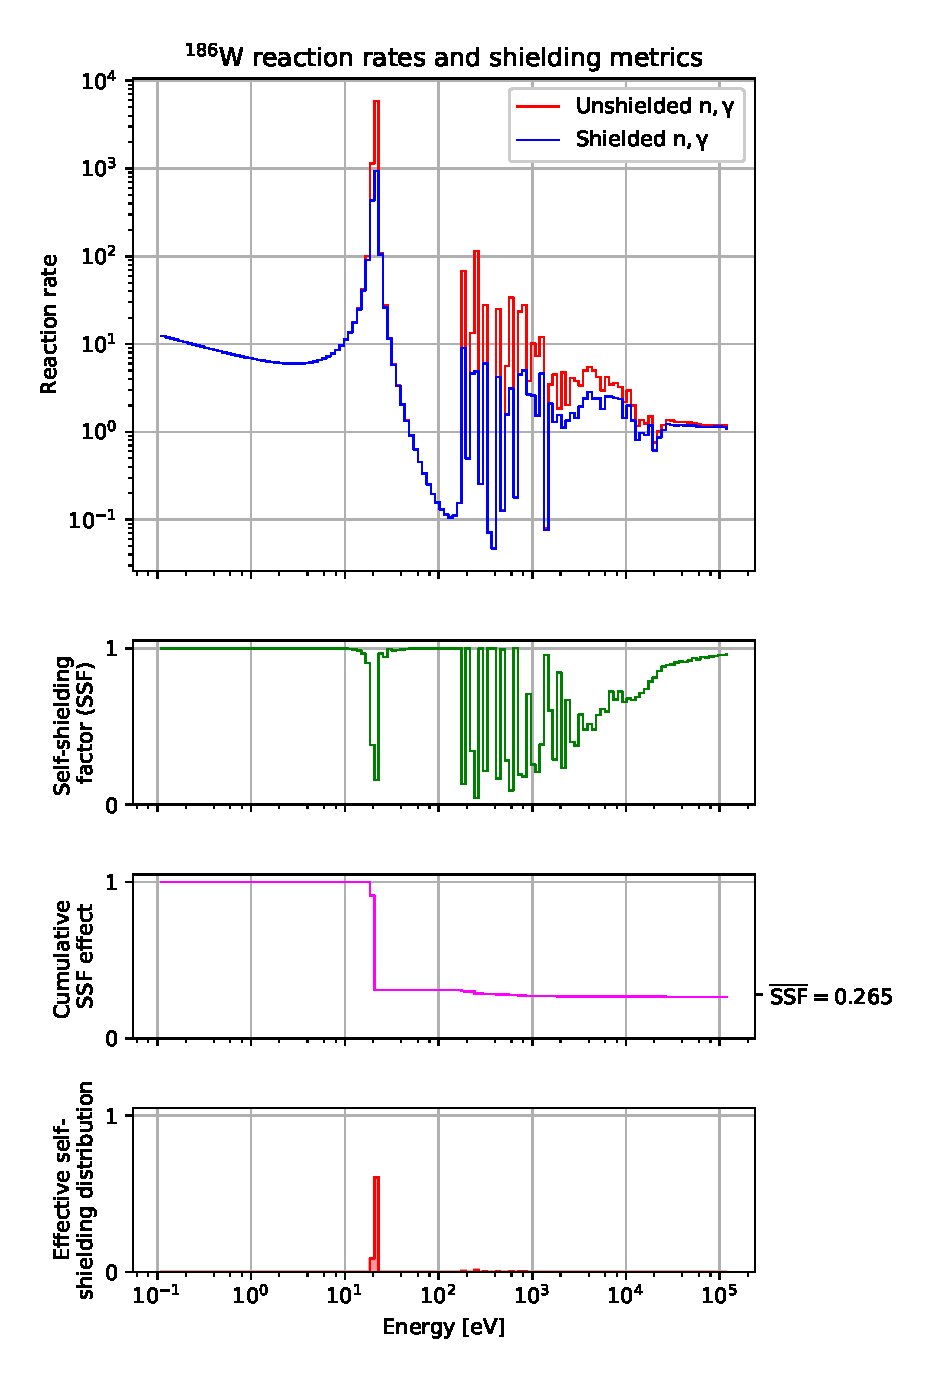
\includegraphics[width=0.8\linewidth]{W186_gamma}
  \caption{Shown in the upper plot is a $^{186}$W radiative capture reaction rate, both unshielded and shielded. The incident particle spectrum in this case is a power function of energy, i.e. $\phi(E) = E^{m}$ where $m$ is some constant, in this case 0. The second plot shows the calculated self-shielding factors as a function of energy for this reaction, given an elemental W material composition. The third plot is the cumulative self-shielding distribution, $C(E_{g})$ from equation~\ref{eq:c}. The fourth and final plot is of, $D(E_{g})$, from equation~\ref{eq:d}.}
  \label{fig:w_cross_section}
\end{figure}

This process of computing $D(E_{g})$ can be repeated for a variety of nuclides and the distributions summed to give their combined effective self-shielding distribution. However, outside the resonance ranges, for example for E $< 10^{-2}$ or E $> 10^{5}$ eV, this distribution is identically zero. To enforce a minimum bin density, a constant, $b$, is added to all bins of $D(E)$ in the algorithm employed. 

\begin{equation}
  \label{eq:b}
  b = \frac{D(E) \Delta E(E)}{\frac{n_{bins}}{bpd_{min}} - d}
\end{equation}

The minimum bins per decade, $\mathrm{bpd}_{min}$ must be specified. Where $d$ is the number of decades described by the group structure, $n_{bins}$ is the total number of bins required of the new group structure and $\Delta E(E)$ is an array of the input group bin widths.

\begin{equation}
  \label{eq:offset}
  \rho(E) = D(E) + b
\end{equation}

$\rho(E)$ is an array of proposed local bin densities, on the input group structure. This is then rebinned into equal areas as per equation \ref{eq:equal} to determine the new, optimised group structure.

\begin{equation}
  \label{eq:equal}
  \int_{g=i-1}^{g=i} \rho(E_{g})dE = \frac{1}{n_\mathrm{bins}}\int_{g=0}^{g=N}\rho(E_{g})dE 
\end{equation} 

An example bin density distribution and the associated new group structure bin bounds are shown in figure~\ref{fig:optimised_bounds}. One can see a greater density of new bin boundaries (green) where the distribution (red) is peaked.

\begin{figure}
  \centering
  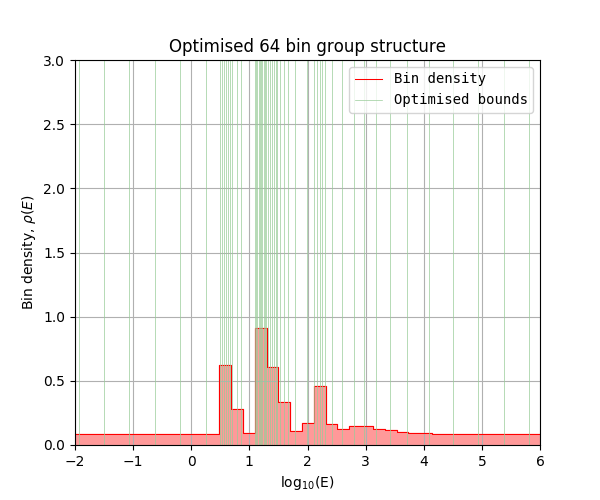
\includegraphics[width=0.8\linewidth]{optimised_bounds}
  \caption{This plot shows the bin density, $\rho(E)$ distribution as per equation~\ref{eq:offset}. This is the summed effective self-shielding distributions for all nuclides of interest, plus some constant to give a minimum bins per decade outside of the resonant region. The 64 log-spaced bin boundaries for this distribution constitute the original group structure. An optimised 64 group structure is determined by rebinning the $\rho(E)$ distribution and is shown by the green lines.}
  \label{fig:optimised_bounds}
\end{figure}

The above process provides a method to determining where a group structure provides a poor representation of the spectra information and nuclides' nuclear physics. It can be used to apportion a given number of bins to construct a new group structure, as shown in equation~\ref{eq:equal} and figure~\ref{fig:optimised_bounds}. However, one needn't stop at this point. With these distributions, other optimisation methods are conceivable. The process can be repeated, in an attempt to converge on an optimum group structure. Or, one might start with a very fine representation, with many tens of thousands of bins and attempt to coarsen based on the effective self-shielding distribution. Section~\ref{subsubsec:iterative} explores these potential methods.

\FloatBarrier
\subsubsection{Iterative and other methods}
\label{subsubsec:iterative}
% Iterative application but also coarsening approaches – all still using some form of rho(E)

% Do I actually have any good results with these `advanced' methods? If not, exclude the method bar a passing remark above...


\subsection{Computation}
\label{subsec:computation}

The calculation of effective cross-sections were carried out using three different techniques:

\begin{enumerate}
  \item Multi-group FISPACT-II unshielded collapse
  \item Multi-group FISPACT-II shielded collapse
  \item Point-wise MCNP6 Monte Carlo Estimator (MCE)
\end{enumerate}

Methods 1 \& 2 discretise the incident spectrum, over a  $\phi(E)$ and $\sigma(E)$, taking the inner product of two vectors of constants,
$$\vec{\phi} \cdot \vec{\sigma} = \sum_i \phi(E_i , E_{i+1}) \sigma(E_i , E_{i+1}),$$
as the spectrum-averaged, effective cross section. However, for each group interval, $(E_{i}, E_{i+1}]$ the true functions $\phi(E),\ \sigma(E)$ are not contant. Regions with resonances in the cross section cause local decreases in the neutron flux, resulting in significant `self-shielding' errors with the multi-group method. To address this, self-shielding factors, $\mathrm{SSF}(E_i)$, may be used to account for these resonance effects. 

An incident spectrum, material inventory and nuclear data are input to FISPACT-II. The spectrum and interaction nuclear data are then collapsed to generate one-group effective cross-sections. With the addition of probability table data generated with CALENDF-2010 \cite{sublet2011}, $\mathrm{SSF}(E_i)$ are calculated for both the resolved and unresolved resonance regions.

Method 3 employs nuclear cross-section data with tens of thousands of points per reaction channel, interpolating between them to approximate a continuous energy treatment. The effective radiative capture cross-section can be determined from the point-wise calculated $(n,\gamma)$ reaction rate as equation \ref{eq:pw}. 

\begin{equation}
\label{eq:pw}
\sigma_\mathrm{eff} = \frac{\int RR_{n,\gamma}(E) dE}{\int \phi(E) dE}
\end{equation}


The effective cross-sections calculated for this study were a series of radiative capture reactions in metals. These reactions often have a large fraction of their total reaction rate within the neutron slowing down region between thermal and fast energies. Hence, an accurate resonance treatment is required for accurate results. 

\subsubsection{Simple test case}
% Concentric spheres used in iterative method, give description of geometry, data and radiation transport

\subsubsection{JET activation foils}
This study tests various group structures against a point-wise reference. We have generated two of the test group structures, attempting to optimise them to accurately calculate reaction rates for a set of nuclides.

The radiation transport geometry utilised in this study is the JET tokamak located near Abingdon, Oxfordshire. Octant 8 of the tokamak has previously housed the Long Term Irradiation Station (LTIS) for exposing activation foils to the JET neutron field. A variety of $(n,\gamma)$ effective cross-sections have been calculated in various materials and for a selection of energy group structures. Some of these group structures are optimised for the materials present in the simulation, while others are standard group structures in common usage today. 

The group structures tested in this study are listed in table \ref{tab:groups}. The two groups, 280 and 650, generated by our process were optimised for all stable nuclides of the following elements: Fe, W, Mo, Nd, Sn, Zr, Cu, Co and Ta. This means we performed the nuclide-wise integral of $\rho(E)$ for all naturally occurring isotopes of these elements. 

\begin{table}[H]
  \centering
  \begin{tabular}{lllll}
    \toprule
    n$_\mathrm{bins}$ & E$_\mathrm{min}$ (eV) & E$_\mathrm{max}$ (eV) & bpd$_\mathrm{res}$ & Description \\ 
    \midrule
    709 & 1E-5 & 1E9 & 50 & CCFE \\
    650 & 1E-5 & 1E8 & 37--101 & Optimised fine \\
    315 & 1E-5 & 1.94E7 & 24--50 & TRIPOLI  \\
    280 & 1E-5 & 1E8 & 11--73 & Optimised coarse \\ 
    175 & 1E-5 & 1.96E7 & 5--22 & VITAMIN-J \\
    \bottomrule
  \end{tabular}
  \caption{Comparison of group structures tested, noting their bin counts, n$_\mathrm{bins}$, the energy range over which they are defined and the bins per decade, bpd$_\mathrm{res}$ they employ in the resonant region.}
  \label{tab:groups}
\end{table}

The reaction channels chosen for study are listed in table \ref{tab:reactions}. The nuclides listed are found in the designs of fusion power systems; iron is the principal constituent of all steels, cobalt a steel impurity which dominates shut down dose rates at intermediate time scales, molybdenum an important steel alloying element, tantalum is being investigated for use in high-heat flux componentry and tungsten is a current first choice for a plasma facing high-heat flux material.

\begin{table}[H]
  \centering
  \begin{tabular}{lll}
    \toprule
    Reaction                                       & E$_\mathrm{first\ res.}$ (eV) & E$_\mathrm{URR}$ (eV) \\ 
    \midrule
    %%$^{58}\mathrm{Fe}(n,\gamma)^{59}\mathrm{Fe}$   & 2.29E2                        & 3.50E5                 \\
    %%$^{59}\mathrm{Co}(n,\gamma)^{60}\mathrm{Co}$   & 1.31E2                        & 1.19E5                \\
    $^{95}\mathrm{Mo}(n,\gamma)^{96}\mathrm{Mo}$   & 4.47E1                        & 5.87E4                \\
    $^{181}\mathrm{Ta}(n,\gamma)^{182}\mathrm{Ta}$ & 4.27E0                        & 4.00E3                \\
    $^{182}\mathrm{W}(n,\gamma)^{183}\mathrm{W}$   & 4.16E0                        & 9.91E4                \\
    $^{186}\mathrm{W}(n,\gamma)^{187}\mathrm{W}$   & 1.88E1                        & 1.21E5                \\ 
    \bottomrule
  \end{tabular}
  \caption{Shown above are the reactions simulated in this study. E$_\mathrm{first\ res.}$ indicates the energy of the first resonant peak in the interaction cross-section. E$_\mathrm{URR}$ defines the end of the resolved resonance range (RRR) and the start of the unresolved resonance range (URR) where experimental energy resolution is insufficient to resolve individual resonances.}
  \label{tab:reactions}
\end{table}

In order to compare the performance of the different group structures, incident particle spectra were obtained. As previously mentioned, the LTIS foil holder is located within Octant 8 of the JET facility. The LTIS MCNP model \cite{lengar2017} was integrated into a reference JET model. The LTIS was populated with foils of the materials noted in table \ref{tab:reactions}. The simulation was set to tally the reaction rates of interest in each of the foils in each specified group structure. Point-wise tallies were also included.

\section{Results \& Discussion}
\label{sec:results}
% Introduce general approach again, tall plot of SSF effect functions is to follow

%%To generate self-shielding factors using FISPACT we require a spectrum. The spectrum shape guess was $\phi(E) = E^{0.192}$, or slightly harder than `flat' (see figure \ref{fig:spectrum} for an indication of the spectrum). 
% Include this test spectrum plot, and the lin-log profile used to bias the SSFs

\subsection{Singly optimised}

A set of sample LTIS spectra are as shown in figure \ref{fig:spectrum}. These particular spectra are from within the tungsten foil. Resonances both within the tungsten and the surrounding materials have resulted in flux depressions. An expanded view of the $^{186}$W 18 eV resonance is shown as figure \ref{fig:spectrum_detail}. The degree to which the resonances are resolved by the different group structures is a function of the bin resolution around the resonance. The 709 group, with a standard 50 bins per decade reaches down into the 18 eV resonance, recording a fluence of 3.5E-9 whilst the optimised group structures, 280 and 650 record 2.32E-9 and 1.26E-9. The standard group structures 175 and 315 which are much coarser in this region record a minimum fluence more than an order of magnitude greater than the 650 group structure.

\begin{figure}[H]
  \centering
  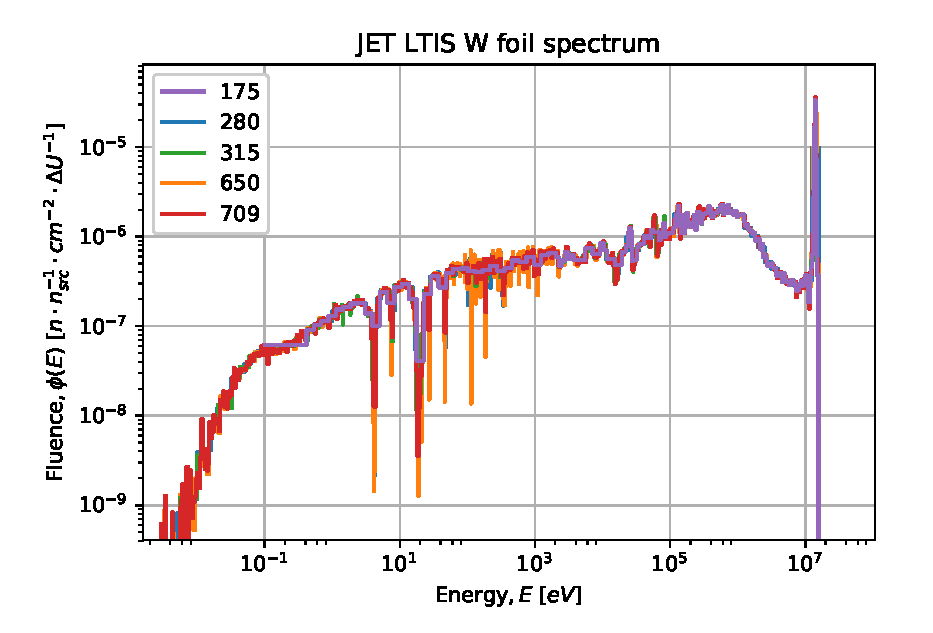
\includegraphics[width=\linewidth]{W186_spectra_diff_groups.eps}
  \caption{Typical DT neutron spectrum within the LTIS activation foil holder. The fluence of each bin has been divided by the lethargy width for that bin, $\Delta U$. The spectrum is hard, with little thermalisation as a consequence the foil's proximity to the plasma. The same neutrons have been binned according to various group structures, from 175 to 709 groups.}
  \label{fig:spectrum}
\end{figure}

\begin{figure}[H]
  \centering
  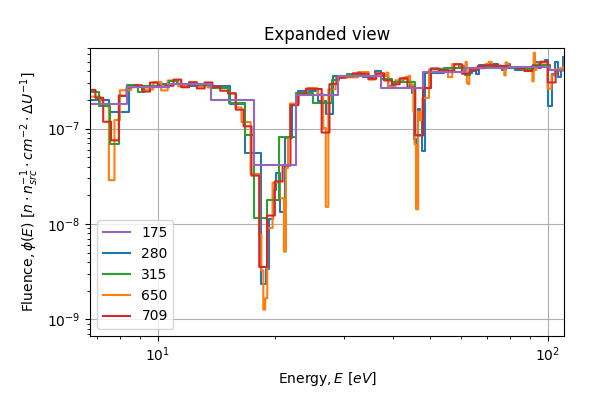
\includegraphics[width=\linewidth]{w_spectrum_detail}
  \caption{Magnified section of spectrum showing how progressively finer group structures resolve flux depressions in a neutron spectrum.}
  \label{fig:spectrum_detail}
\end{figure}

Figure \ref{fig:tungsten-182} shows a comparison of collapsed cross-sections for $^{182}$W. The abscissa lists each group structure tested. A pair of data points exist for each group structure, one with the use of self-shielding factors (shielded) and one without (unshielded). The abscissa order is a sorted such that the unshielded values decrease from left to right. The left ordinate indicates the absolute cross-section value in barns, while the right ordinate gives the cross-section as a percentage change over the point-wise (reference) value, i.e. +100\% means the multi-group calculation has over-estimated the cross-section and therefore reaction rate by a factor of 2.

As would be expected, in a simple, unshielded case having more groups and therefore a larger number of groups per energy decade tends to give multi-group results closer to the reference point-wise result. Flux depressions are better resolved with narrower groups and therefore the reaction rate resulting from resonances is not overestimated to the same degree. However, with the exception of $^{181}$Ta, the 650 optimised group, and even the 280 optimised group perform better than the 709 group in the unshielded regime. Their narrow groups are targeted where most useful, around the resonances which were poorly described by a equal logarithmically spaced group structure.

\begin{figure}[H]
  \centering
  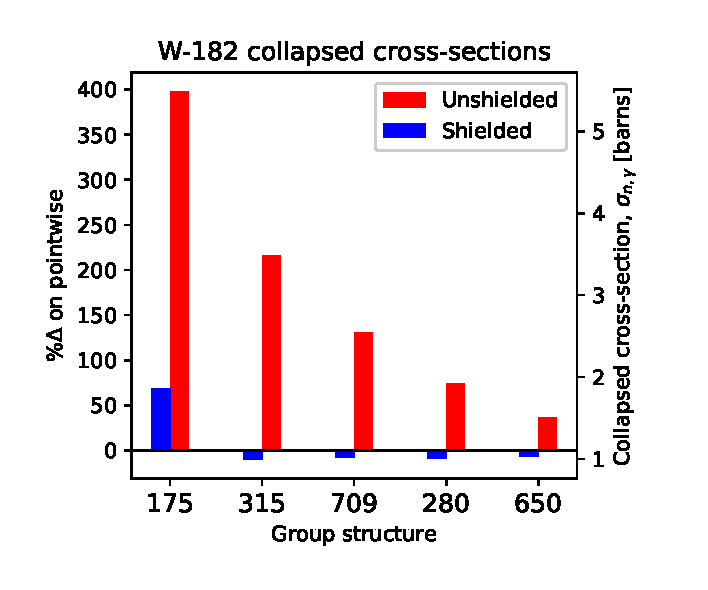
\includegraphics[width=\linewidth]{W-182.eps}
  \caption{Comparison of different calculation methods for radiative capture in $^{182}$W under JET neutron irradiation.}
  \label{fig:tungsten-182}
\end{figure}

With regards to individual groups, the 175 group used unshielded performs very poorly, overestimating the reaction rate by at least a factor of 3 in all cases. The 650 optimised group is always within 50\% of the point-wise result and is the best performing group.

\begin{figure}[H]
  \centering
  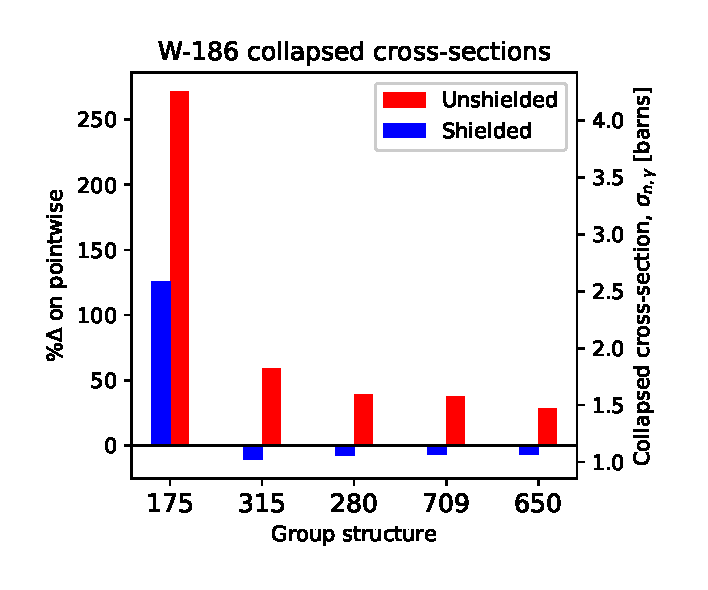
\includegraphics[width=\linewidth]{W-186.eps}
  \caption{Comparison of different calculation methods for radiative capture in $^{186}$W under JET neutron irradiation.}
  \label{fig:tungsten-186}
\end{figure}

As might be expected the shielded results show far less variation between groups. 280, 315, 650 \& 709 demonstrate largely similar behaviour when used in conjunction with self-shielding factors. 175 does again over-estimate, between 0\% and 120\% depending on the nuclide.

\begin{figure}[H]
  \centering
  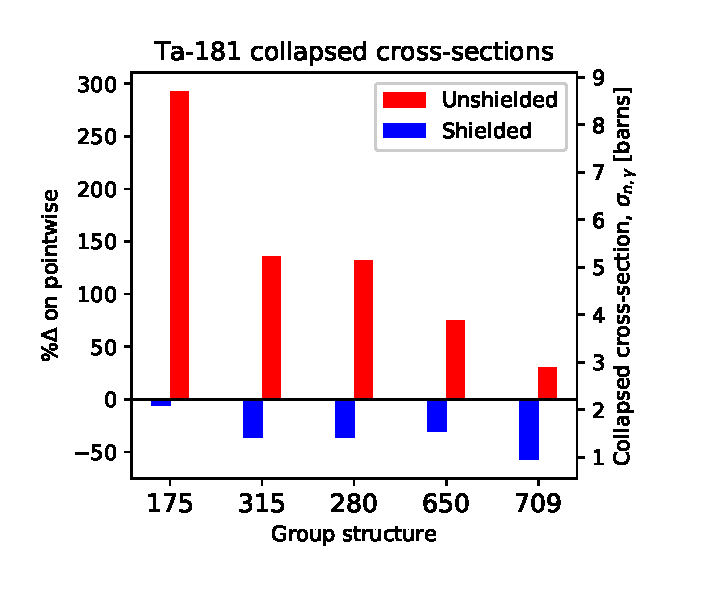
\includegraphics[width=\linewidth]{Ta-181.eps}
  \caption{Comparison of different calculation methods for radiative capture in $^{181}$Ta under JET neutron irradiation.}
  \label{fig:tantalum-181}
\end{figure}

The $^{181}$Ta (figure \ref{fig:tantalum-181}) and $^{95}$Mo (figure \ref{fig:molybdenum-95}) results indicate over-shielding, that is self-shielding factors over compensating for a poor description of the spectrum. This is particularly pronounced for the 315 group in $^{95}$Mo, where the shielded result is 40\% less than the point-wise result. This is due to the application of one set of self-shielding factors over the entirety of the foil depth. Although only 500 microns, the compound geometric effects are essential and are the subject of further work.

\begin{figure}[H]
  \centering
  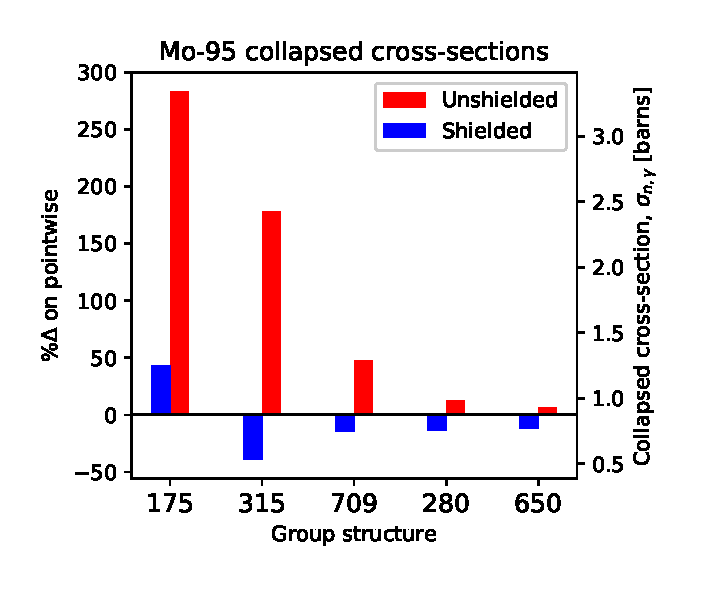
\includegraphics[width=\linewidth]{Mo-95.eps}
  \caption{Comparison of different calculation methods for radiative capture in $^{95}$Mo under JET neutron irradiation.}
  \label{fig:molybdenum-95}
\end{figure}

\subsection{Advanced methods}
% Results from iteratively applying algorithm, coarsening vs. straight rho(E), etc.


\section{Conclusions}

This study has investigated how an incident spectrum and nuclear data library are discretised in energy (i.e. the group structure) effects the accuracy of reaction rate calculations. The selection of group structures trialled included three in current use and two which were optimised by our own, novel method.

The accuracy of multi-group reaction rate calculations is severely hampered by using the legacy VITAMIN-J 175 group structure. In the context of this activation foil problem, coarse group structures can give reasonable results if used in conjunction with modifying self-shielding factors. If used, self-shielding factors must be applied carefully, with potential geometric shielding effects considered. If used inappropriately, over-shielding may result, which may not be conservative depending on the context.

An optimisation algorithm has been demonstrated. The algorithm can generate and optimised set of bin bounds, given a `guess' spectrum and a target nuclide set. An unshielded multi-group calculation using an optimised group structure with 280 bins has more closely approximated the point-wise result than the 709 unshielded multi-group calculation in the majority of cases examined.

Further work will improve on the optimisation algorithm and explore the performance of optimised group structures in a wider array of circumstances. Iterative application of the algorithm will be investigated as well as geometric self-shielding effects. 


%!TEX root = ../thesis.tex
%*******************************************************************************
%****************************** Concluding Chapter *****************************
%*******************************************************************************

\chapter{Concluding remarks} %Title of last chapter
\label{chap:conclusion}

\ifpdf
    \graphicspath{{Chapter4/Figs/Raster/}{Chapter4/Figs/PDF/}{Chapter4/Figs/}}
\else
    \graphicspath{{Chapter4/Figs/Vector/}{Chapter4/Figs/}}
\fi

%********************************** %First Section  **************************************

This thesis has explored the causes and effects of several uncertainties in nuclear fusion reactor analysis and operation. It began by describing motivations for developing controlled nuclear fusion power, by situating new power generation technologies within a broader environmental and socio-political context. A growing world population demanding improving material living standards has increased global power demand to double its value of 40 years ago. Human-induced climate change, deteriorating air quality and a desire for greater energy security have helped spur the development of low-carbon electricity production technologies such as renewables, GEN-IV fission and fusion to meet contemporary and future demands for power.

Whilst the body of nuclear fusion knowledge has massively accumulated since the process was first discovered, constructing and operating a working fusion reactor, as opposed to an experiment, is still yet to happen. However we are now in the final stages of research and development before such a reactor is constructed and it is tremendously important to identify and quantify any risks to the realisation of controlled nuclear fusion as an economical, practical electricity generation scheme. Many of these risks are political and organisational, but as the introductory chapter alluded to, many are technical, engineering challenges. Hopefully none are physical impossibilities. 

Many of the technical risks are amplified by our inexact knowledge of them. A tremendous amount of work is currently undertaken to model the performance of current and future fusion devices, simulating performance and estimating parameters of interest. However, these parameters are always subject to some sort of uncertainty, whether it is quoted or not. Uncertainty in powers, Mean Time Between Failures (MTBF), particle fluxes, cost of electricity, Tritium Breeding Ratios and more. To decrease these uncertainties, to narrow their distribution around the most mean value, is to reduce the maximum potential risk associated with them and to give room for manoeuvre in the trade-offs that come with engineering a functioning system. 

The work which comprises this thesis has investigated several sources of uncertainty of pertinence to the development of nuclear fusion as a power generation scheme. First, a stochastic, sampling technique known as Total Monte Carlo was used to explore the effects of nuclear data uncertainty in the TBR for a future fusion power plant design, DEMO. This technique has never before been used to estimate uncertainty on TBRs. Investigating the contribution of uncertainty from lead nuclear data, many radiation transport simulations of the DEMO device were performed, each tallying the TBR and sampling different lead nuclear data. This work used the TENDL2015 nuclear dataset, with fully correlated cross-channel behaviour for the reaction channels, angular distributions and other variables. The results of the work were to determine the standard deviation of the HCLL DEMO TBR due to lead, 1.2\% of the mean value. The simulated TBR distribution was not normally distributed, instead it had a negative skewness--a low-value tail. As a result, 5.8\% of the TBR distribution was less than unity. This only serves to reinforce the importance of higher-order moments in parameter probability distributions and the value of TMC style methods. Generally, where parameter mean values are close to the limits of some operational range, one should seek to know the shape of that parameter distribution, not just the extent. Whilst a TBR in a liquid-metal breeder blanket could potentially be tailored through on-line $^{6}$Li enrichment, this is not the case for ceramic type breeding concepts. For those, an overestimated TBR could be a costly mistake. After sampling the TBR distribution, the relationships between fundamental nuclear parameters and the TBR were investigated, with a handful of local Optical Model Potential (OMP) parameters responsible for most of the variation in TBR. In terms of future research, the determination of uncertainty contributions to TBR in lead blankets from other nuclides such as $^{16}$O, $^{56}$Fe and $^{nat.}$W would be a worthwhile effort. Advances in theory or new nuclear physics experimental data could help refine our models of lead nuclei and their behaviour, reducing uncertainties in lead based blanket designs.

The subsequent chapter looked at a particular modelling approximation, spatial homogenisation, where heterogeneity in material composition is artificially reduced by replacing many realistic materials with mass-conserving mixtures of materials. The effects of this approximation on radiation shielding were investigated. First the basic theory of radiation shielding was introduced, before a description of a comparative method for determining the discrepancy between heterogeneous and homogeneous modelling approaches. This method was employed to analyse how the approximation affects calculated dose rates for parameters relevant to the ITER tokamak. In one scenario, the on-load dose rate from D-T fusion was calculated on the far side of a reinforced concrete wall similar to the ITER bio-shield. The discrepancy induced by the homogeneous approximation was a function of wall thickness, and attained a maximum of a 22\% underestimate of the neutron dose. This underestimate in the homogeneous simulation is due to the dispersed absorbing nuclei from the steel material which act as neutron sinks. There was less effect for photons, with a maximum underestimate of 10\%. The impacts of spatial homogenisation on the Shut-Down Dose Rate (SDDR) were also investigated. Activation at the internal face of the shield was found to be overestimated by a small amount by spatial homogenisation, approximately 10\%, although this did vary as a function of time since last irradiation. The effects of spatial homogenisation in breeding blankets for fusion have been explored by \citeauthor{Pelloni1989} amongst others \cite{Kumar1989}. However, these results pertaining to radiation shielding in nuclear systems are novel, with no similar study having been published before. 

Finally, an exploration of energy domain discretisation, or `group structure optimisation' was undertaken. How the energy domain is subdivided for nuclear analyses can have a significant effect on results. Previous methods for optimisation were mentioned, along with a discussion of nuclear resonant behaviour and the phenomenon of self-shielding. Having developed a framework for the generation of nuclear data on an arbitrary group structure, a method for the targeting of bin density is devised. The method starts with a logarithmically-spaced group structure and determines where self-shielding modifications to cross-sections most impact reaction rates. Distributions of effective self-shielding in energy are computed and summed for chosen nuclides. This distribution is then used as the basis for a bin density distribution and the apportioning of the energy domain. The method is applied to optimise group structures for two cases, a simple tungsten example and a more general group, optimised for a variety of metals of importance to fusion. Both conferred a significant advantage over traditional group structures in common usage today. The optimised 280 bin group structure was used to determine reaction rates in JET activation foils more accurately than the CCFE 709 bin group structure. Future work could involve the testing of optimised general group structures, to see if advantages are still conferred when optimisation is for a very large population of nuclides. Iterative applications of the algorithm were investigated during the course of this work, but did not confer any advantage of single applications. One alternative, related route for optimisation could be using the effective self-shielding distributions as defined in this work, but starting from hyper-fine groups and removing the least necessary bounds until a target is reached. This approach may waste fewer bins than going from relatively coarse to locally fine, as is done in the current implementation.

Nuclear analyses are subject to a variety of sources of uncertainty. These can be from nuclear data, modelling approximations, discretisation of variables, amongst many other factors. Often these sources are simultaneously present in problems. \citeauthor{El-Guebaly2009}'s study of contributions to TBR uncertainty in lithium-lead blankets asserts that 90\% of the TBR margin required is to account for uncertainty in its estimation, only the remaining fraction is the required net gain for system losses \cite{El-Guebaly2009}. The uncertainty comes from both nuclear data (60\%) and modelling (30\%). Sometimes modelling approximations are synergistic in effect, as \citeauthor{Pelloni1989} noted that failing to account for self-shielding effects in breeding calculations is particularly important with homogenised geometries \cite{Pelloni1989}. 

Minimising uncertainty will become more important as we move towards constructing the first demonstration fusion devices, as unexpected or poor performance may reduce the momentum of these projects. We can continue to reduce sources of uncertainty in nuclear analyses through the development of improved methods, such as the energy group structure optimisation presented here. If approximations must be made for issues of limited computation, as with spatial homogenisation, then further analysis of the effects will be necessary to ensure their effects are adequately understood. Lastly, quantifying parameter distributions through the application of uncertainty propagation techniques like TMC will likely see an increased role--expanding from solely ND to sample other sorts of input distributions, perhaps including manufacturing tolerances and other parameters.









%\include{Chapter5/chapter5}
%\include{Chapter6/chapter6}
%\include{Chapter7/chapter7}



% ********************************** Back Matter *******************************
% Backmatter should be commented out, if you are using appendices after References
%\backmatter


% ********************************** Appendices ********************************

\begin{appendices} % Using appendices environment for more functunality

%!TEX root = ../thesis.tex
% ******************************* Thesis Appendix A ****************************
\chapter{Radiation shielding material definitions} 
\label{app:materials}

\section*{Concrete}

\begin{table}[H]
  \centering
  \begin{tabu} to 0.3\textwidth {X X}
    \toprule
    Element   &   \% weight \\
    \midrule
    H & 0.56 \\
    O & 49.75 \\
    Na & 1.71 \\
    Mg & 0.26 \\
    Al & 4.69 \\
    Si & 31.47 \\
    S & 0.13 \\
    K & 1.92 \\
    Ca & 8.28 \\
    Fe & 1.24 \\
    \bottomrule
  \end{tabu}
  \caption[Concrete material composition]{Concrete composition \% weight from \cite{Jakhar16}. The H content may be overestimated in this mixture. Sampling suggests it may be as low as 0.2\%wt \cite{Aramburu16}. The consequences of such an deviation are substantial and were investigated in work not presented here.}
  \label{tab:concrete}
\end{table}

\newpage

\section*{Steel (radiation transport)}

\begin{table}[H]
  \centering
  \begin{tabu} to 0.3\textwidth {X X}
    \toprule
    Element & \% weight \\
    \midrule
    Fe & 97.24 \\
    C & 0.22 \\
    P & 0.05 \\
    S & 0.05 \\
    N & 0.012 \\
    Mn & 0.56 \\
    Cr & 0.16 \\
    Mo & 0.16 \\
    V & 0.16 \\
    Ni & 0.7 \\
    Cu & 0.7 \\
    \bottomrule
  \end{tabu}
  \caption[Steel material composition for radiation transport]{Steel composition \% weight from \cite{BSsteel05}.}
  \label{tab:steel}
\end{table}

\newpage

\section*{Steel (activation)}

\begin{table}[H]
  \centering
  \begin{tabu} to 0.3\textwidth {X X}
    \toprule
    Element & \% weight \\
    \midrule
    Fe & 97.613 \\
    C  & 0.22 \\
    P  & 0.05 \\
    S  & 0.05 \\
    N  & 0.012 \\
    Mn & 1.08 \\
    Cr & 0.1 \\
    Mo & 0.01 \\ 
    V  & 0.005 \\
    Ni & 0.05 \\
    Cu & 0.8 \\
    Co & 0.01 \\
    \bottomrule
  \end{tabu}
  \caption[Steel composition for activation-transmutation.]{Steel composition \% weight for SDDR calculations from \cite{Barabash16}. This composition includes minor constituents which are not important for radiation transport, but may play a significant role in any SDDR.}
  \label{tab:sddr_steel}
\end{table}



\end{appendices}

% *************************************** Nomenclature ********************************
\printnomenclature


% ********************************** Bibliography ******************************
\begin{spacing}{0.9}

% To use the conventional natbib style referencing
% Bibliography style previews: http://nodonn.tipido.net/bibstyle.php
% Reference styles: http://sites.stat.psu.edu/~surajit/present/bib.htm

\bibliographystyle{apalike}
%\bibliographystyle{unsrt} % Use for unsorted references  
%\bibliographystyle{plainnat} % use this to have URLs listed in References
\cleardoublepage
\bibliography{References/references} % Path to your References.bib file


% If you would like to use BibLaTeX for your references, pass `custombib' as
% an option in the document class. The location of 'reference.bib' should be
% specified in the preamble.tex file in the custombib section.
% Comment out the lines related to natbib above and uncomment the following line.

%\printbibliography[heading=bibintoc, title={References}]


\end{spacing}

% *************************************** Index ********************************
\printthesisindex % If index is present


\end{document}

